\subsubsection{EVEN and ODD} \label{sssec:skipp}

Figures \ref{fig:EVEN_QuantiB} (a) and \ref{fig:ODD_QuantiB} (a), quantifiers related to the normalized histogram of values slightly degrades with the skipping procedure due to finite data length.
For example $\left\langle H_{val}\right\rangle $ reduces from $0.9722$ without skipping to $0.9459$ for EVEN and $0.9706$ for ODD. 
This difference between EVEN and ODD in floating point is because a high dispersion was obtained for $H_{val}$, $H_{BP}$ and $C_{BP}$ but not for $H_{BPW}$ or $C_{BPW}$.

Figs. \ref{fig:EVEN_QuantiB} (b) to \ref{fig:EVEN_QuantiB} (f) and Figs. \ref{fig:ODD_QuantiB} (b) to \ref{fig:ODD_QuantiB} (f) show the results of BP and BPW quantifiers for EVEN and ODD respectively.
Higher accuracy is required to achieve lower complexity than without using skipping.
From the MP point of view a great improvement is obtained using any of the skipping strategies but ODD is slightly better than EVEN.
Missing patterns are reduced to $MP = 118$ for EVEN and ODD, increasing the maximum allowed Bandt \& Pompe entropy that reaches the mean value $\left\langle H_{BP}\right\rangle  = 0.8381$ for EVEN, and $\left\langle H_{BP}\right\rangle  = 0.9094$.
The complexity is reduced to $\left\langle C_{BP}\right\rangle = 0.224$ for EVEN and $\left\langle C_{BP}\right\rangle = 0.282$ for ODD.
The necessary number of bits to converge to this value is $B>40$ for both EVEN and ODD maps.

\begin{figure}
	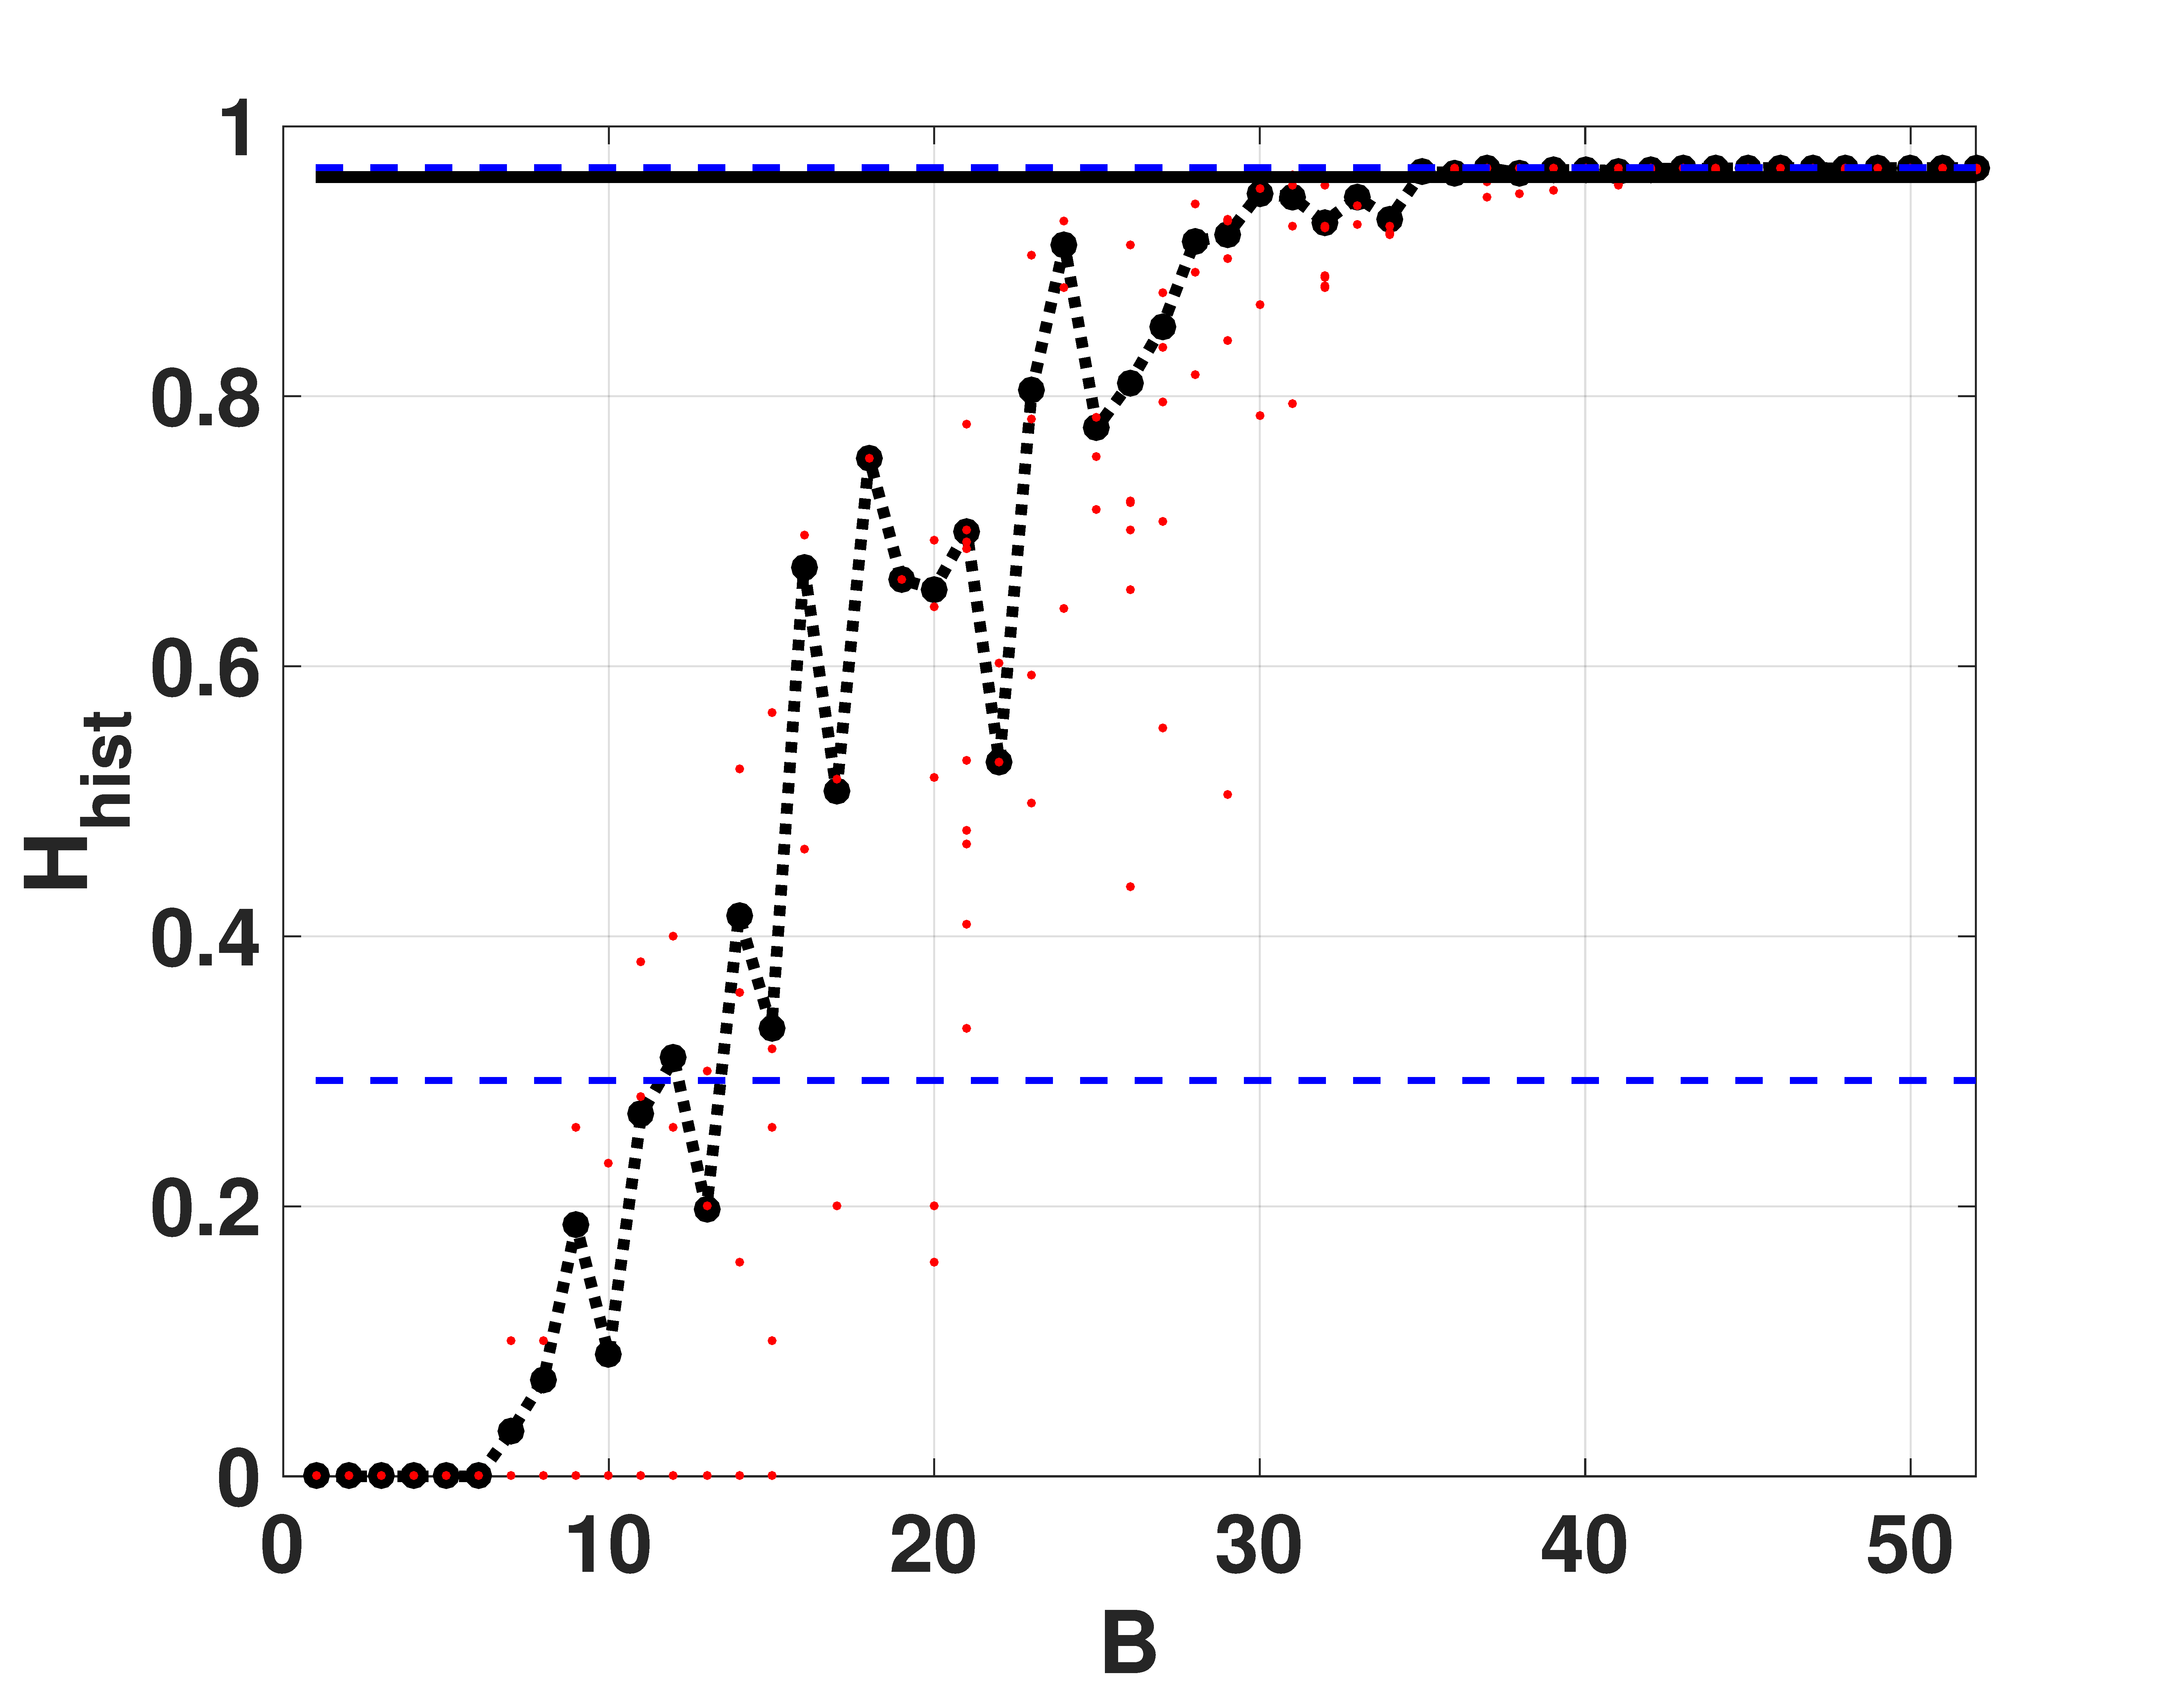
\includegraphics[width=.49\textwidth]{Hval_Even}
	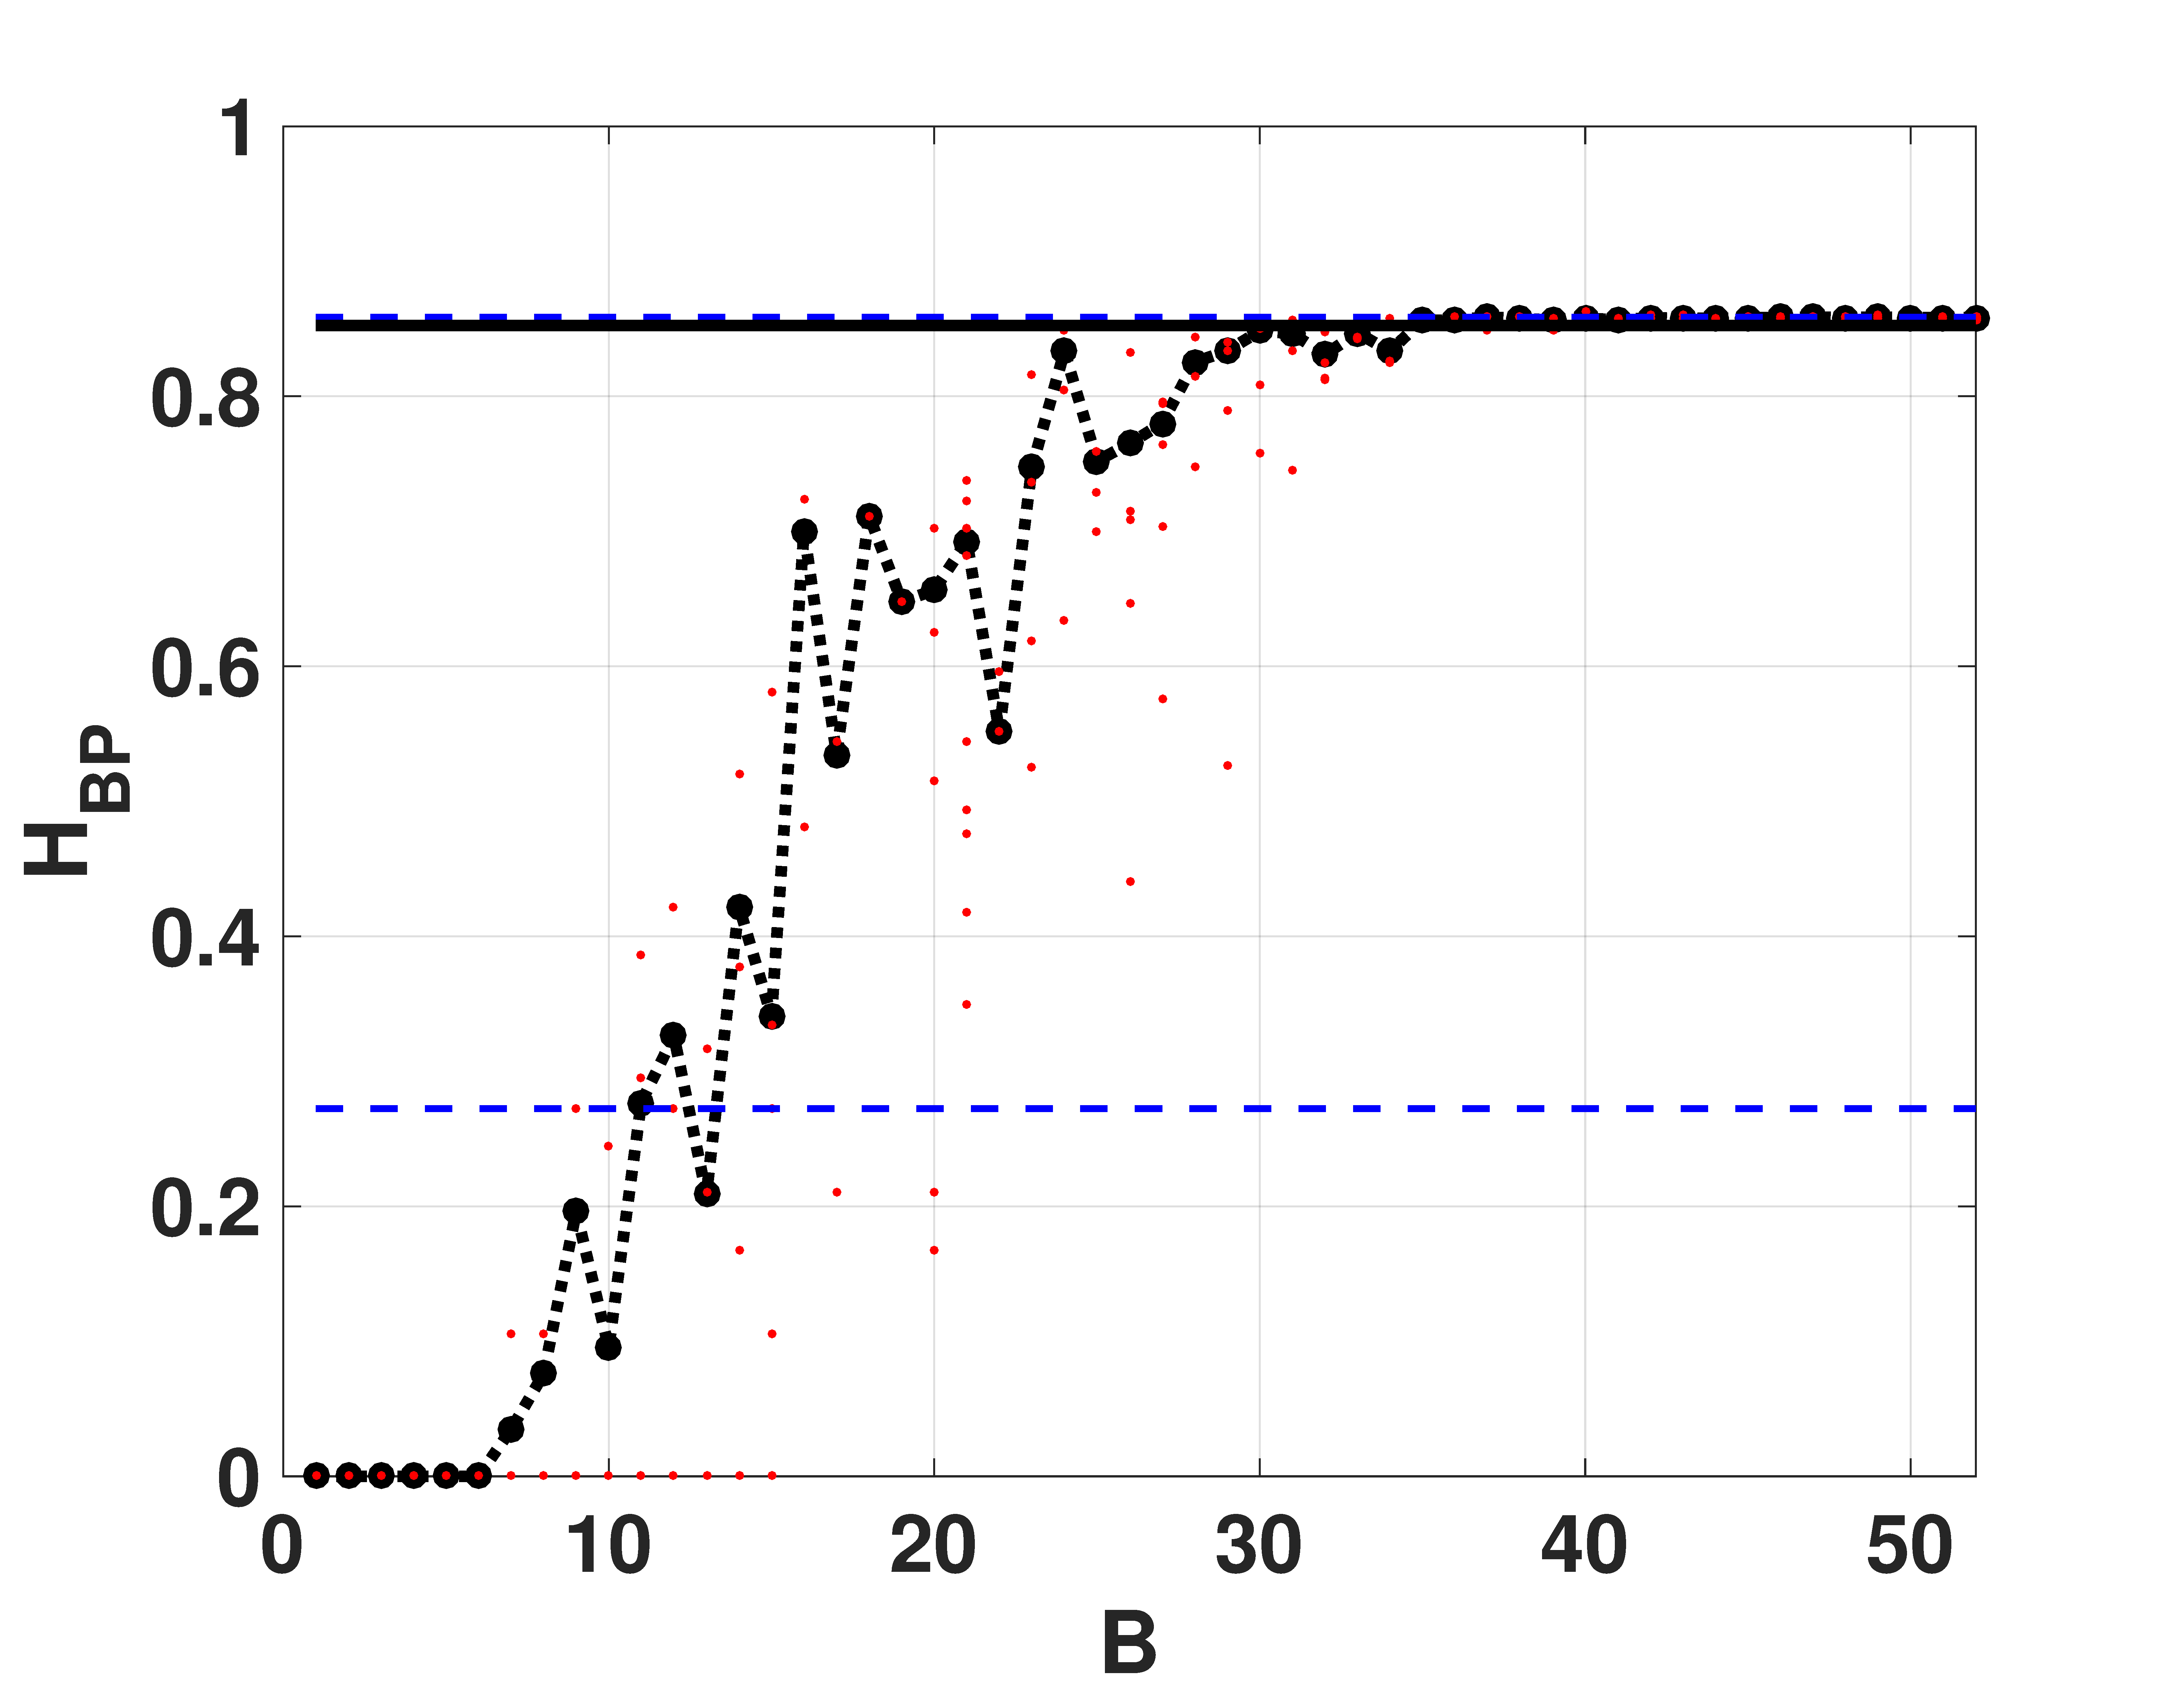
\includegraphics[width=.49\textwidth]{Hbp_Even}
	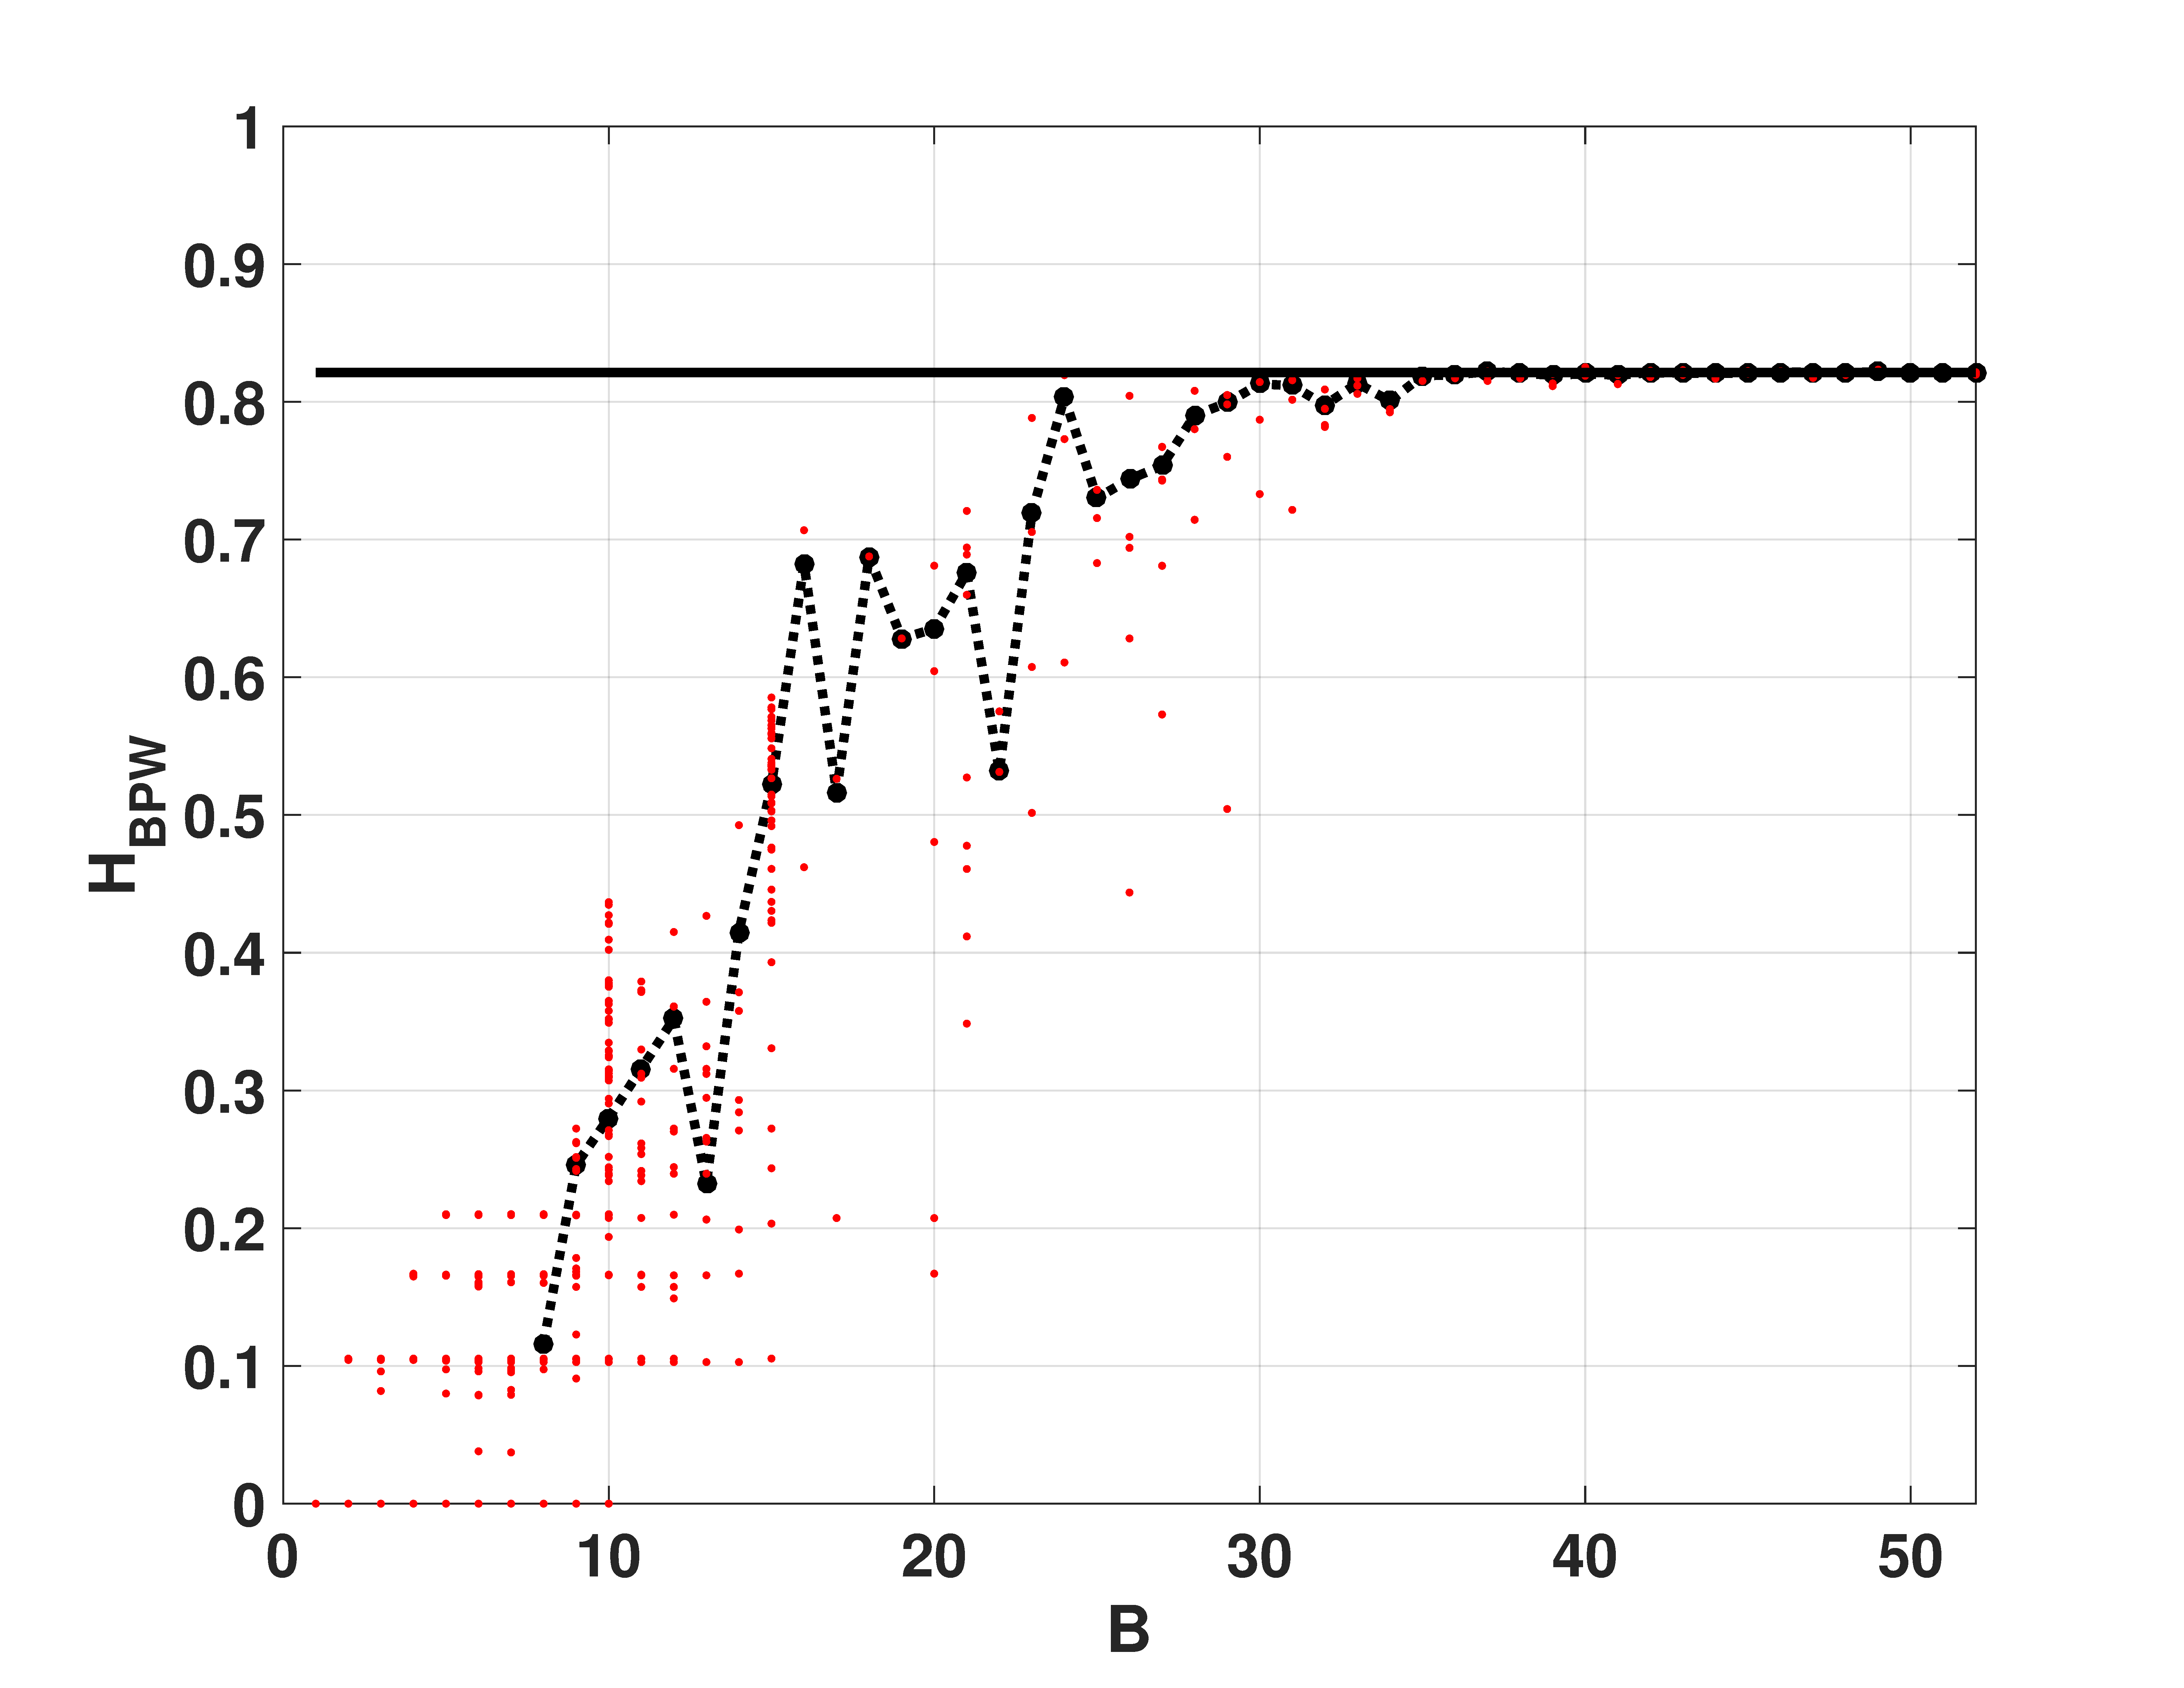
\includegraphics[width=.49\textwidth]{Hbpw_Even}
	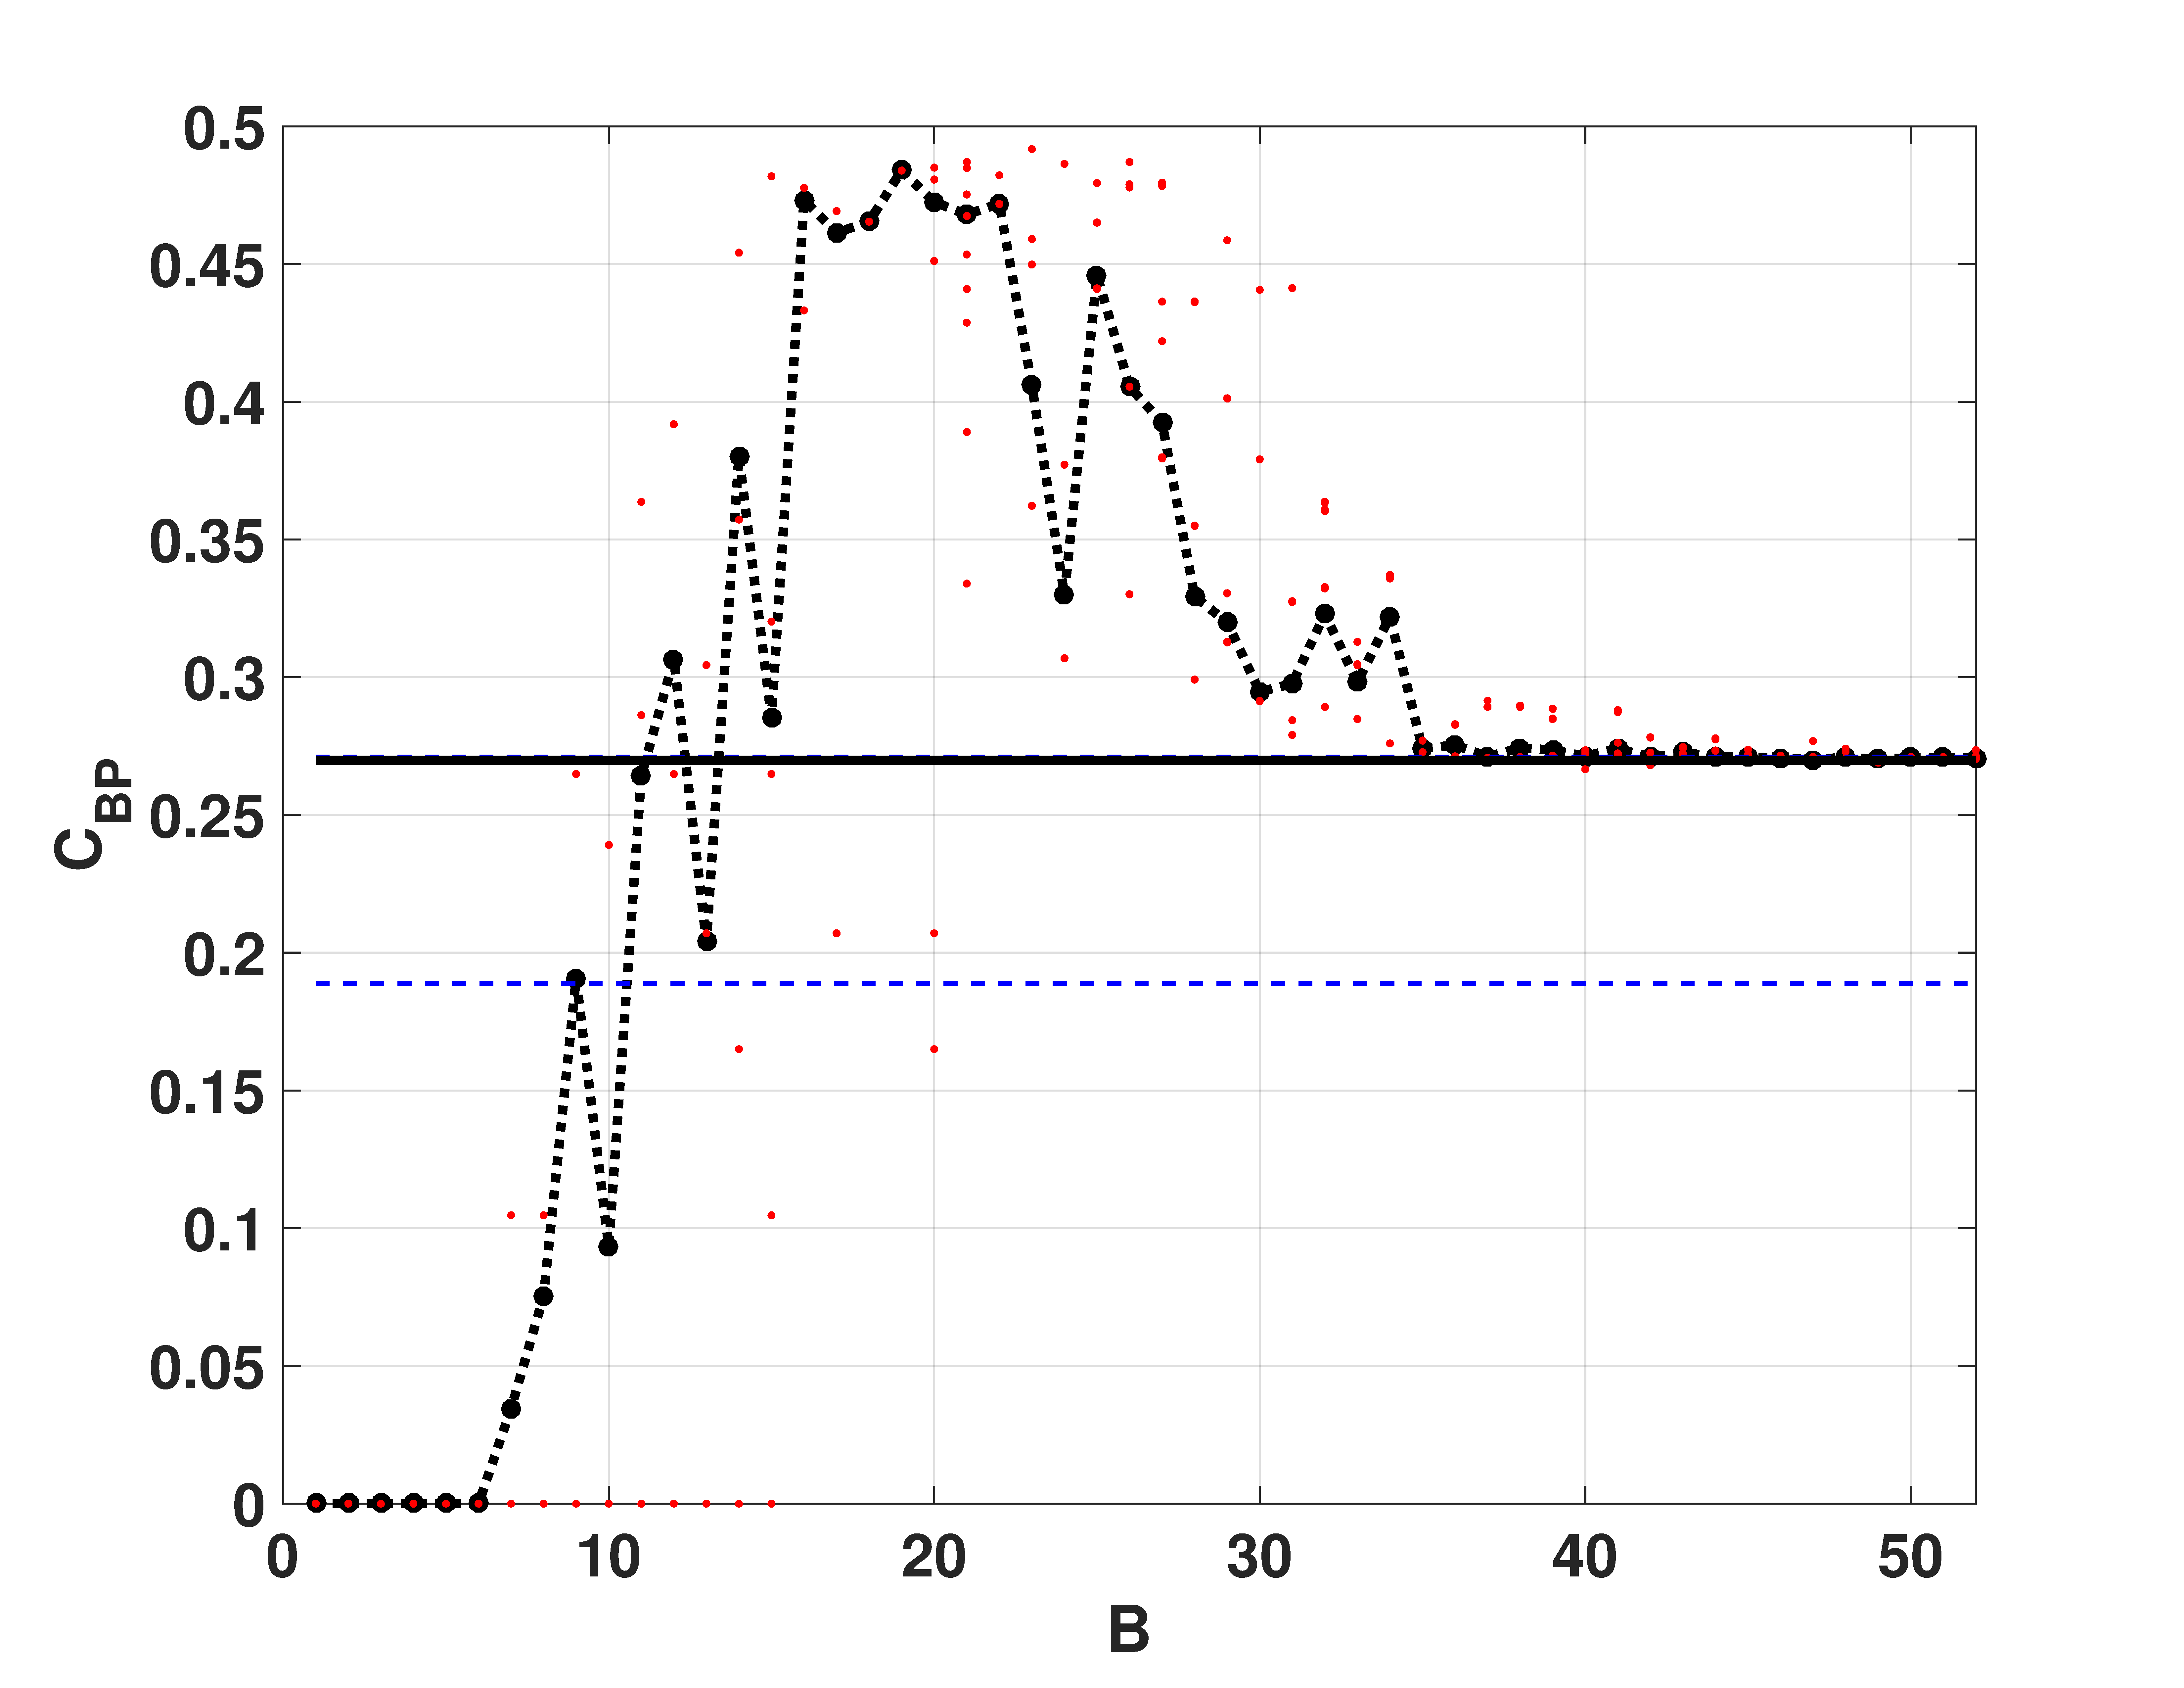
\includegraphics[width=.49\textwidth]{Cbp_Even}
	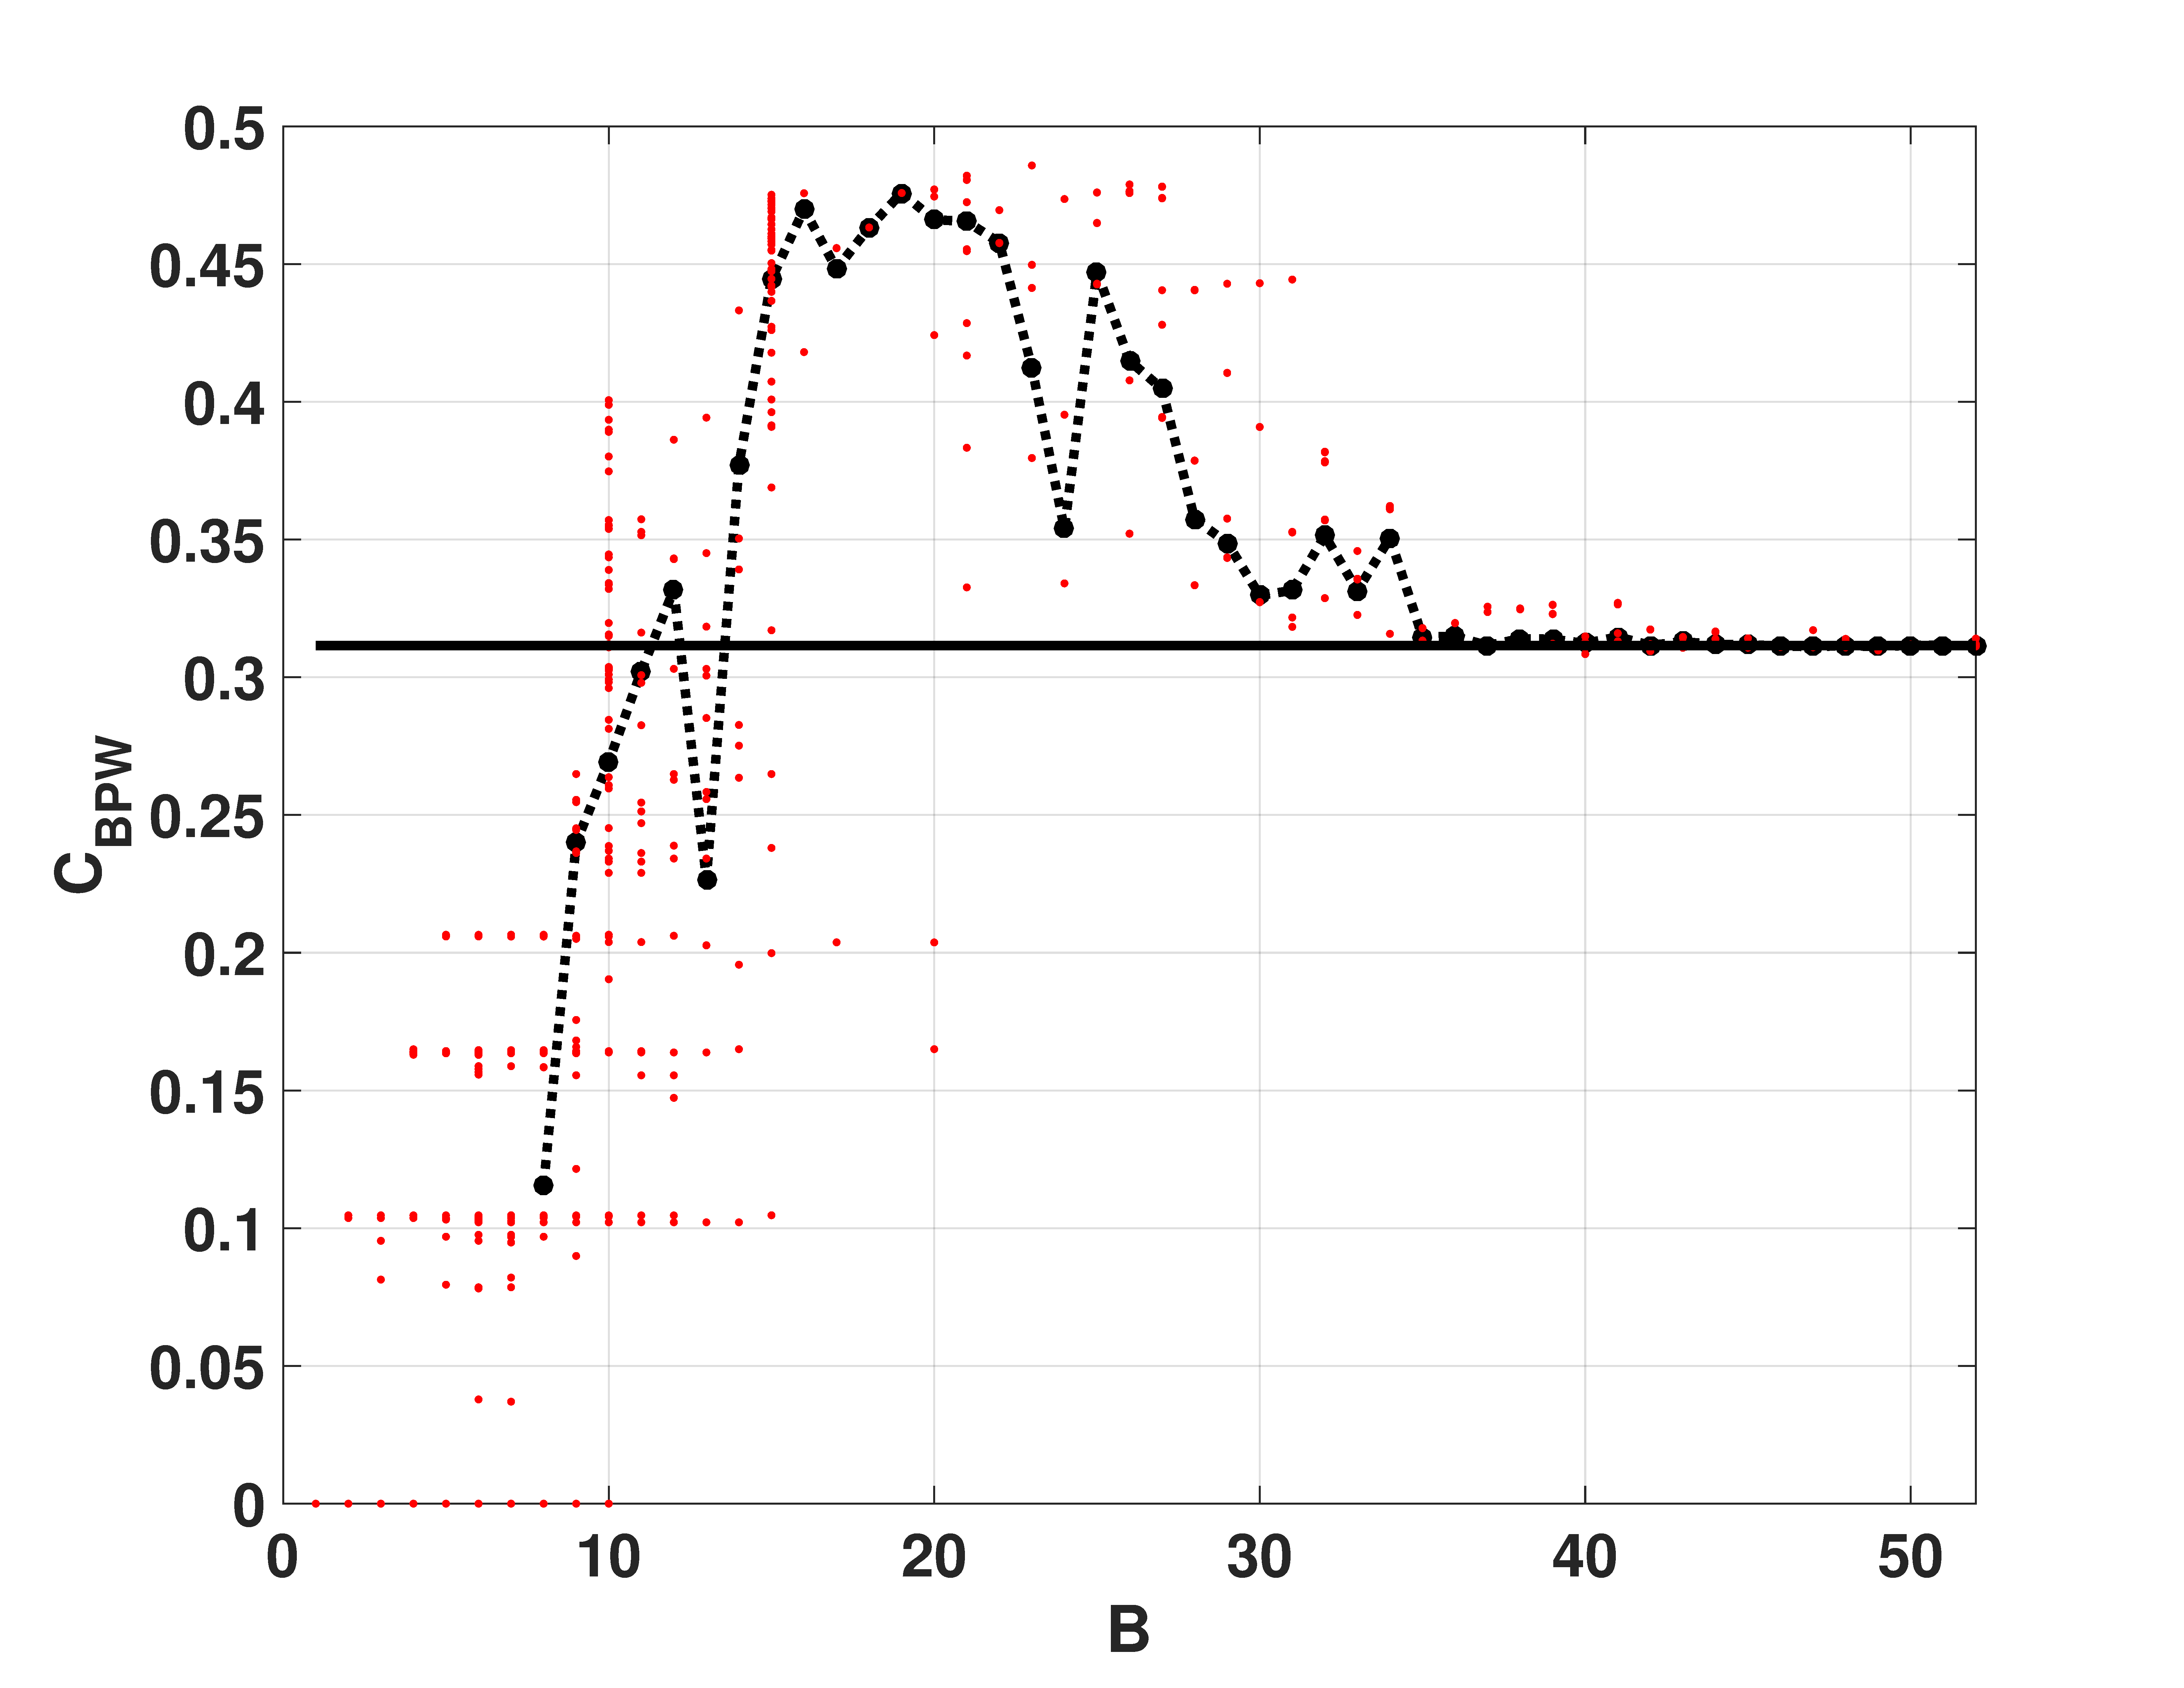
\includegraphics[width=.49\textwidth]{Cbpw_Even}
	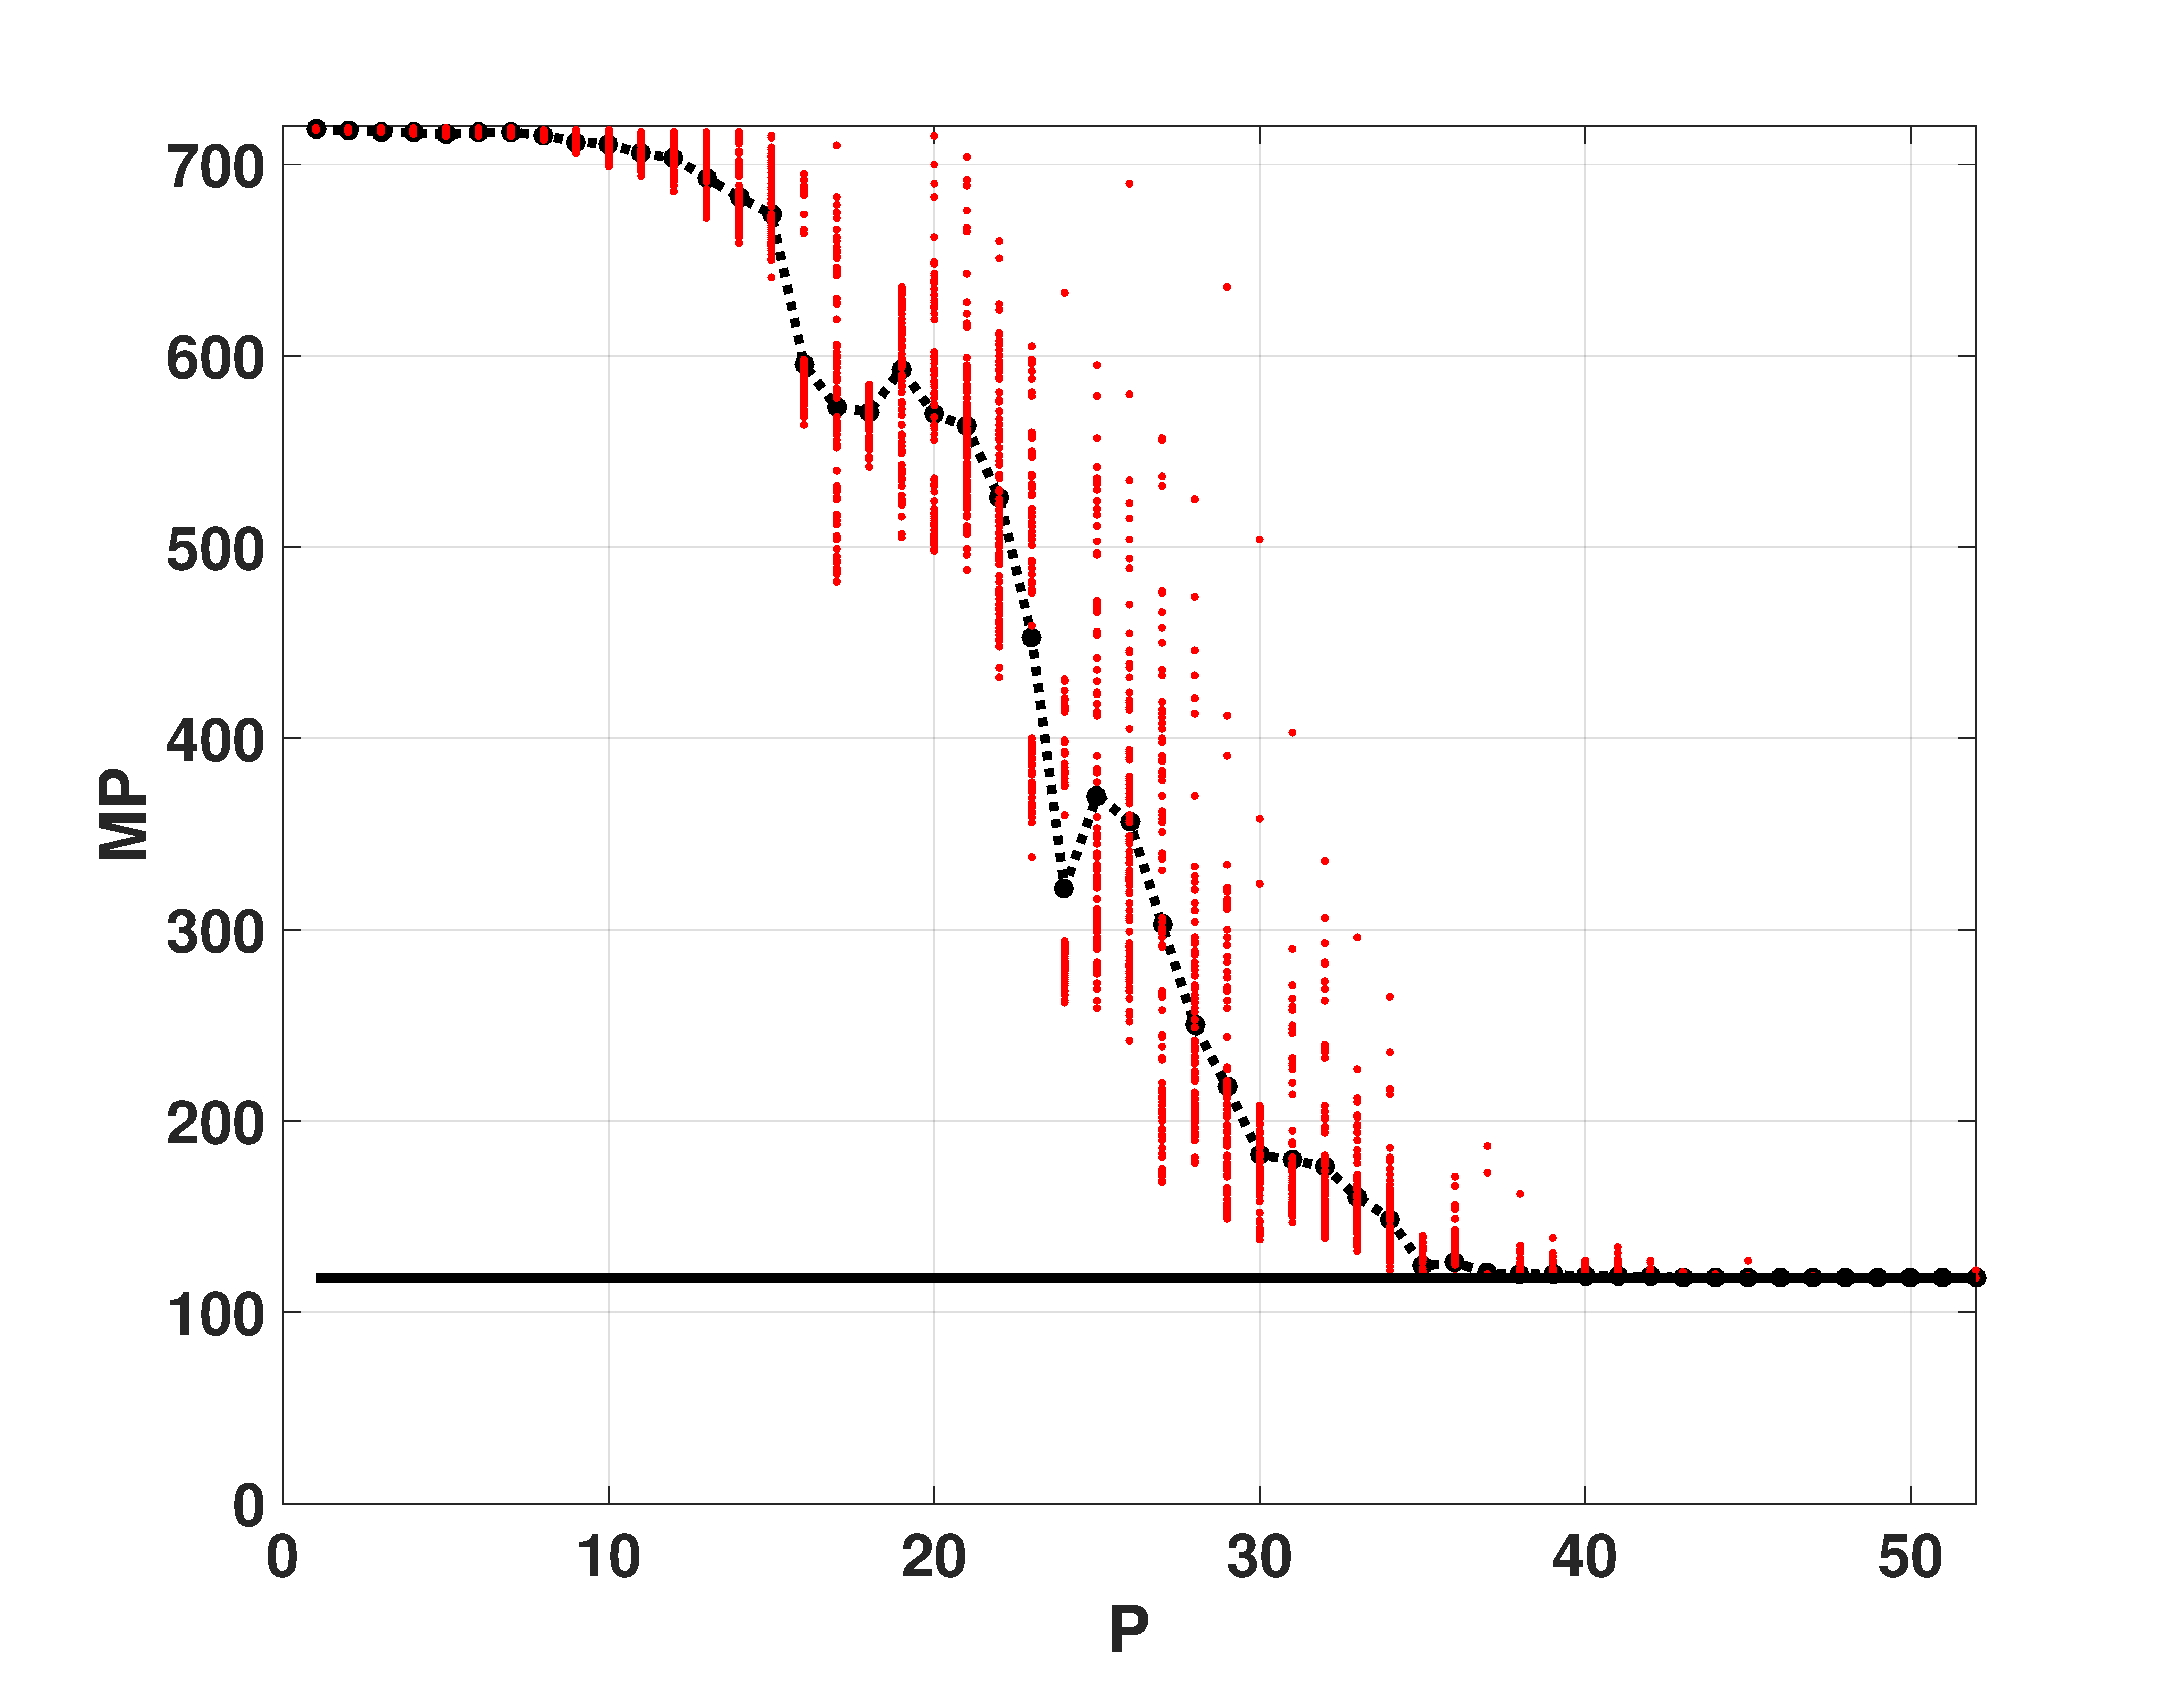
\includegraphics[width=.49\textwidth]{MP_Even}
	\caption{Statistical properties of the EVEN map: (a) $H_{val}$ vs $B$ (b) $H_{BP}$ vs $B$ (c) $C_{BP}$ vs $B$ (d) $MP$ vs $B$.}
	\label{fig:EVEN_QuantiB}
\end{figure}

\begin{figure}
	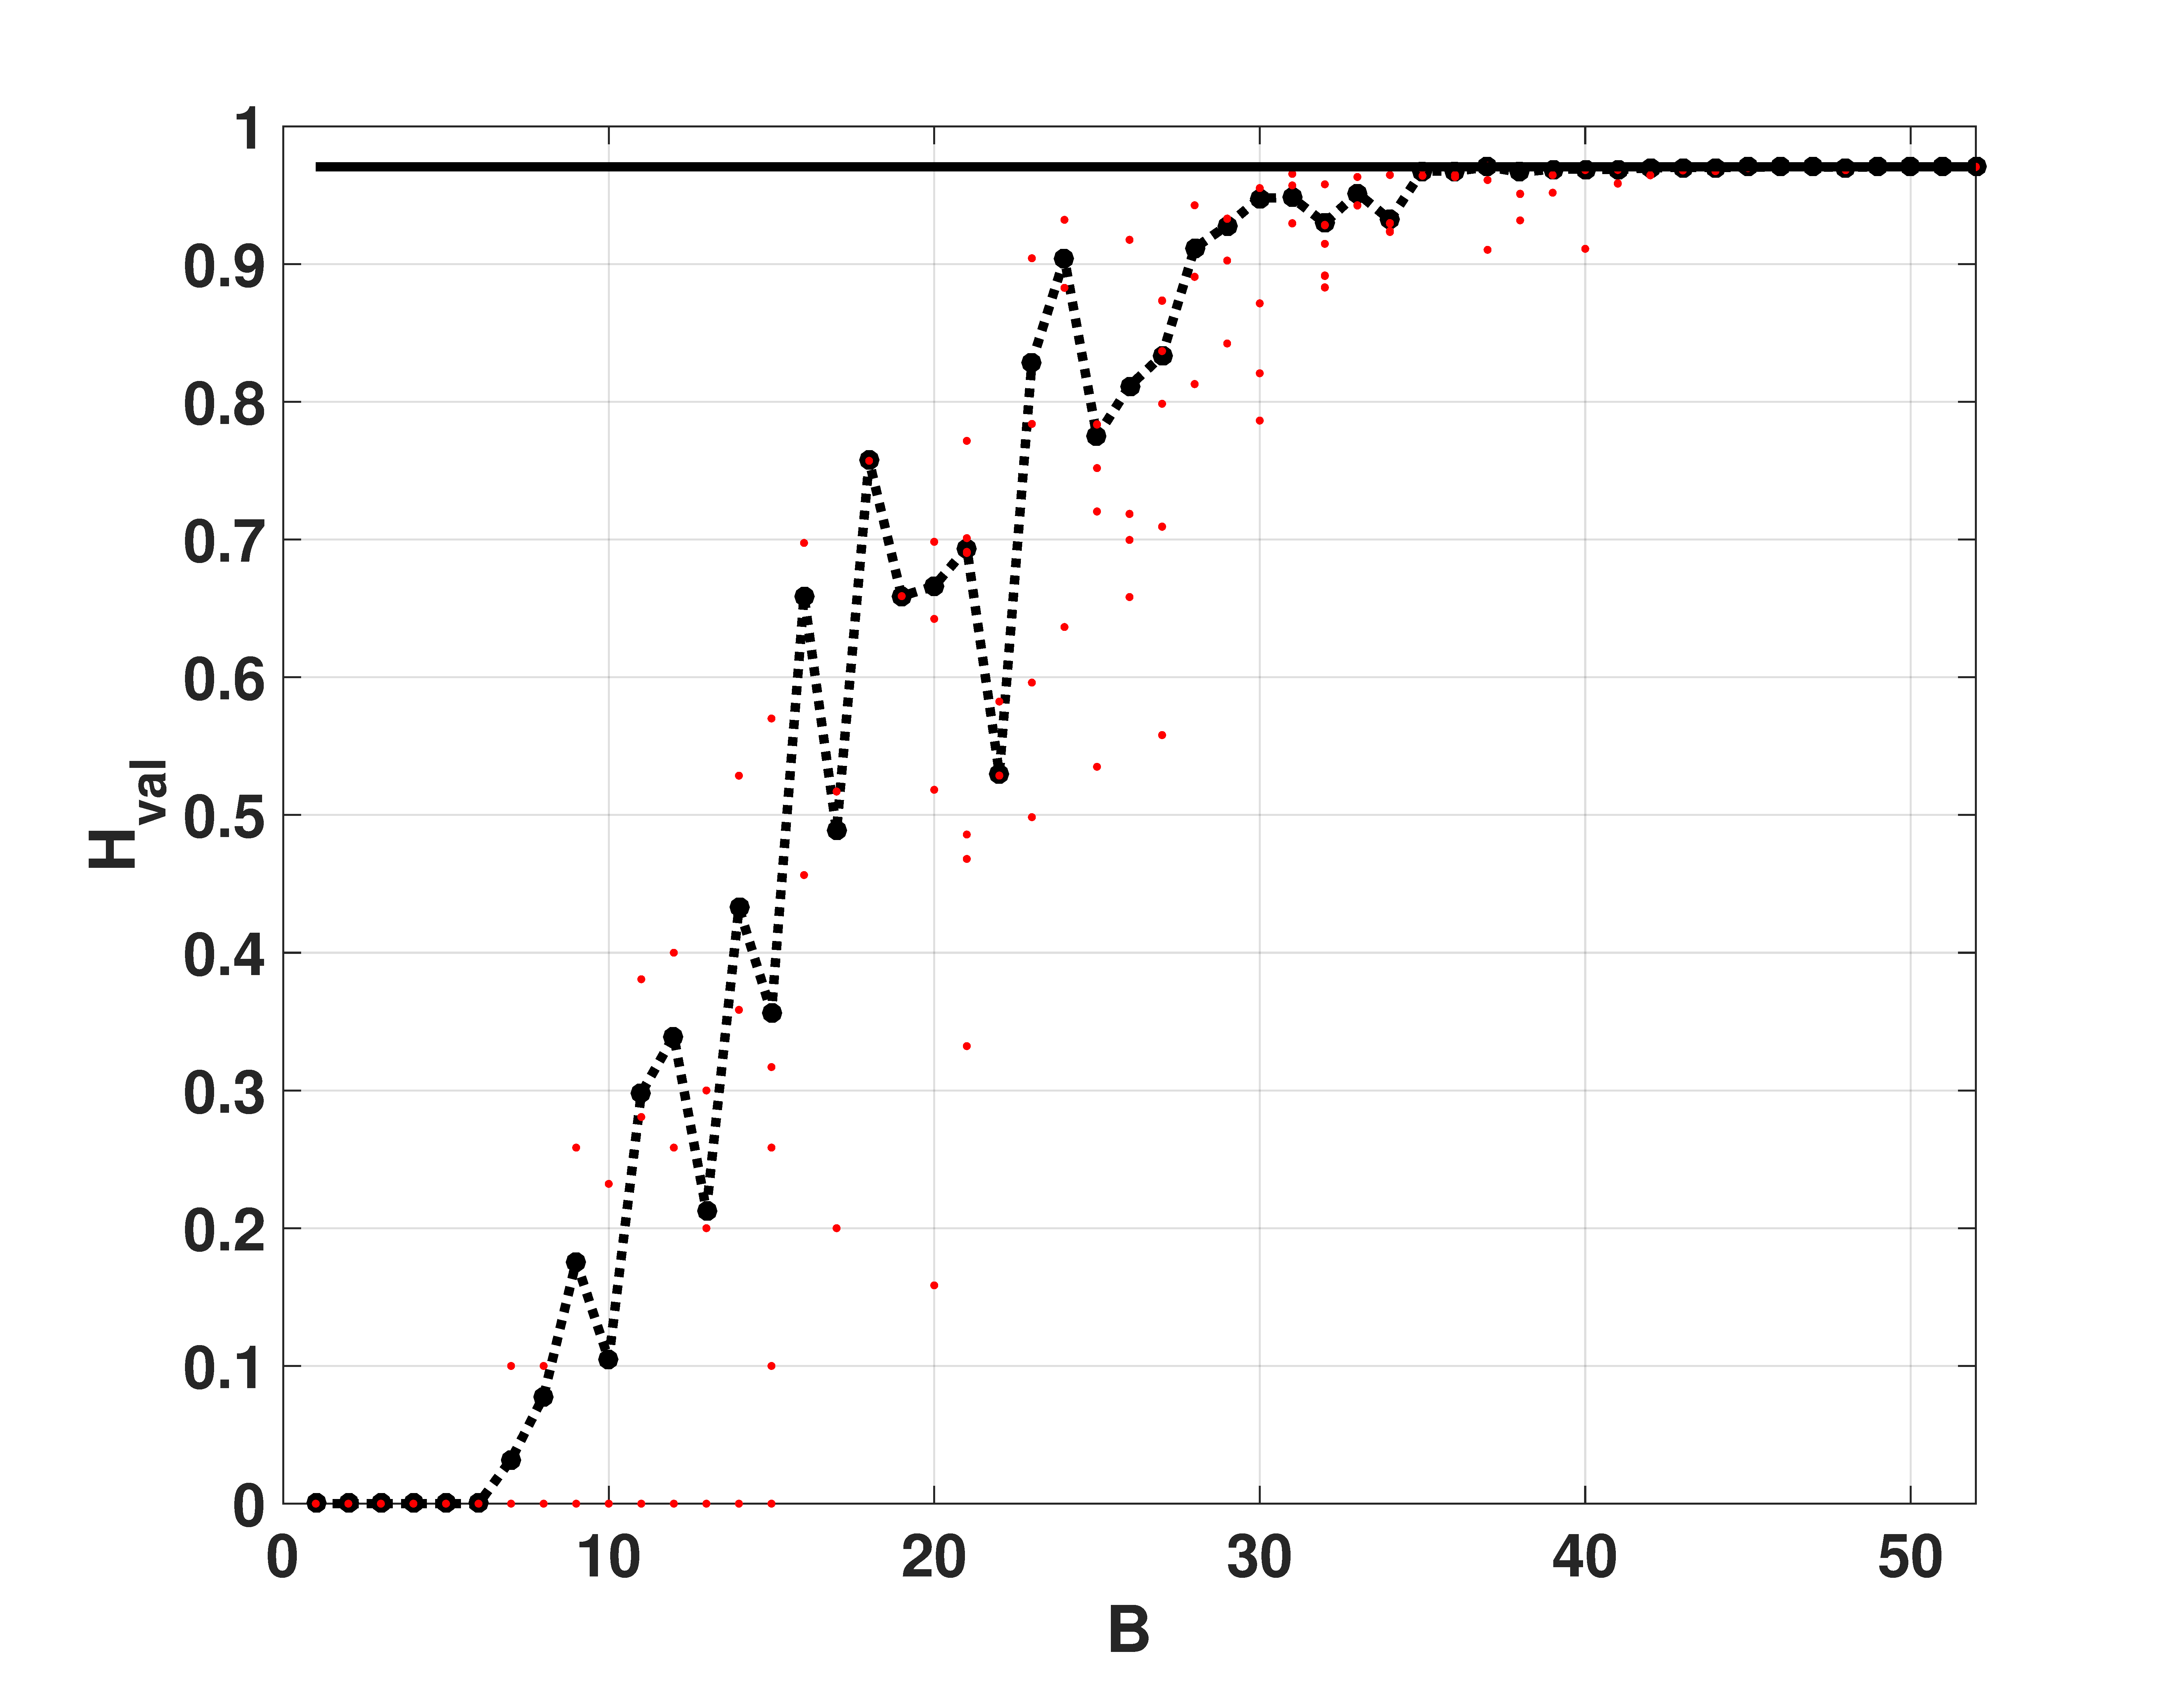
\includegraphics[width=.49\textwidth]{Hval_Odd}
	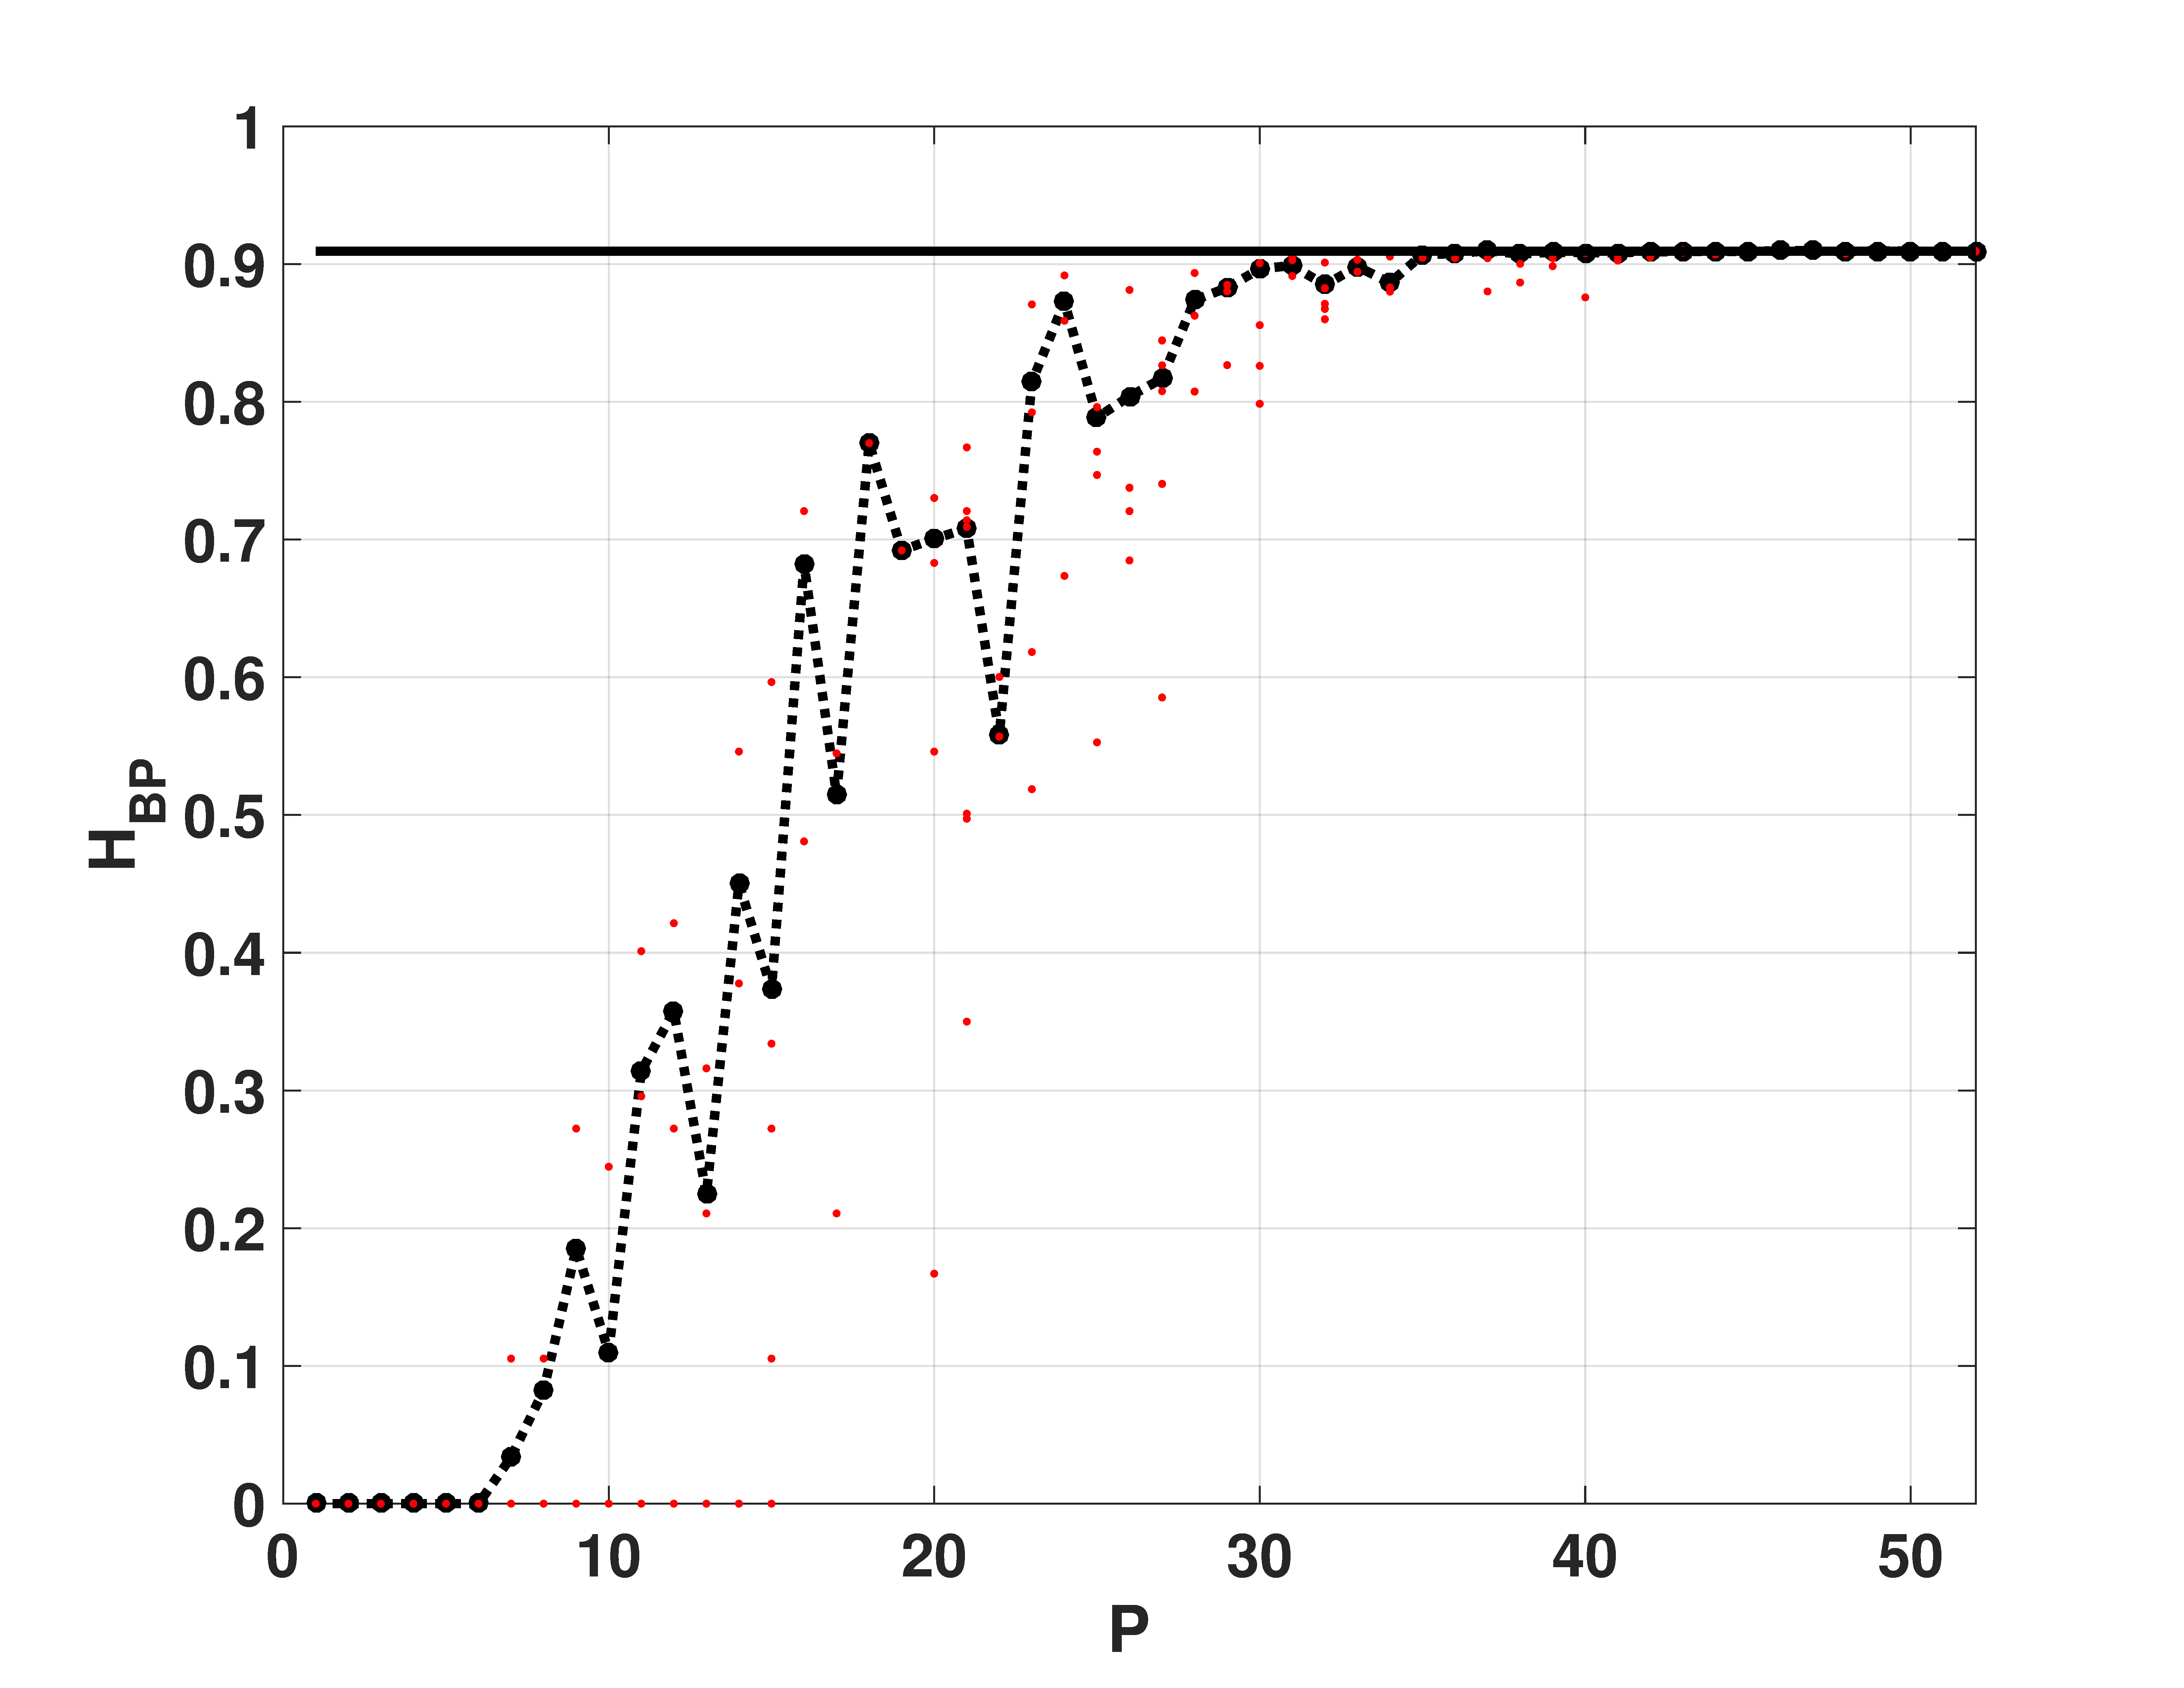
\includegraphics[width=.49\textwidth]{Hbp_Odd}
	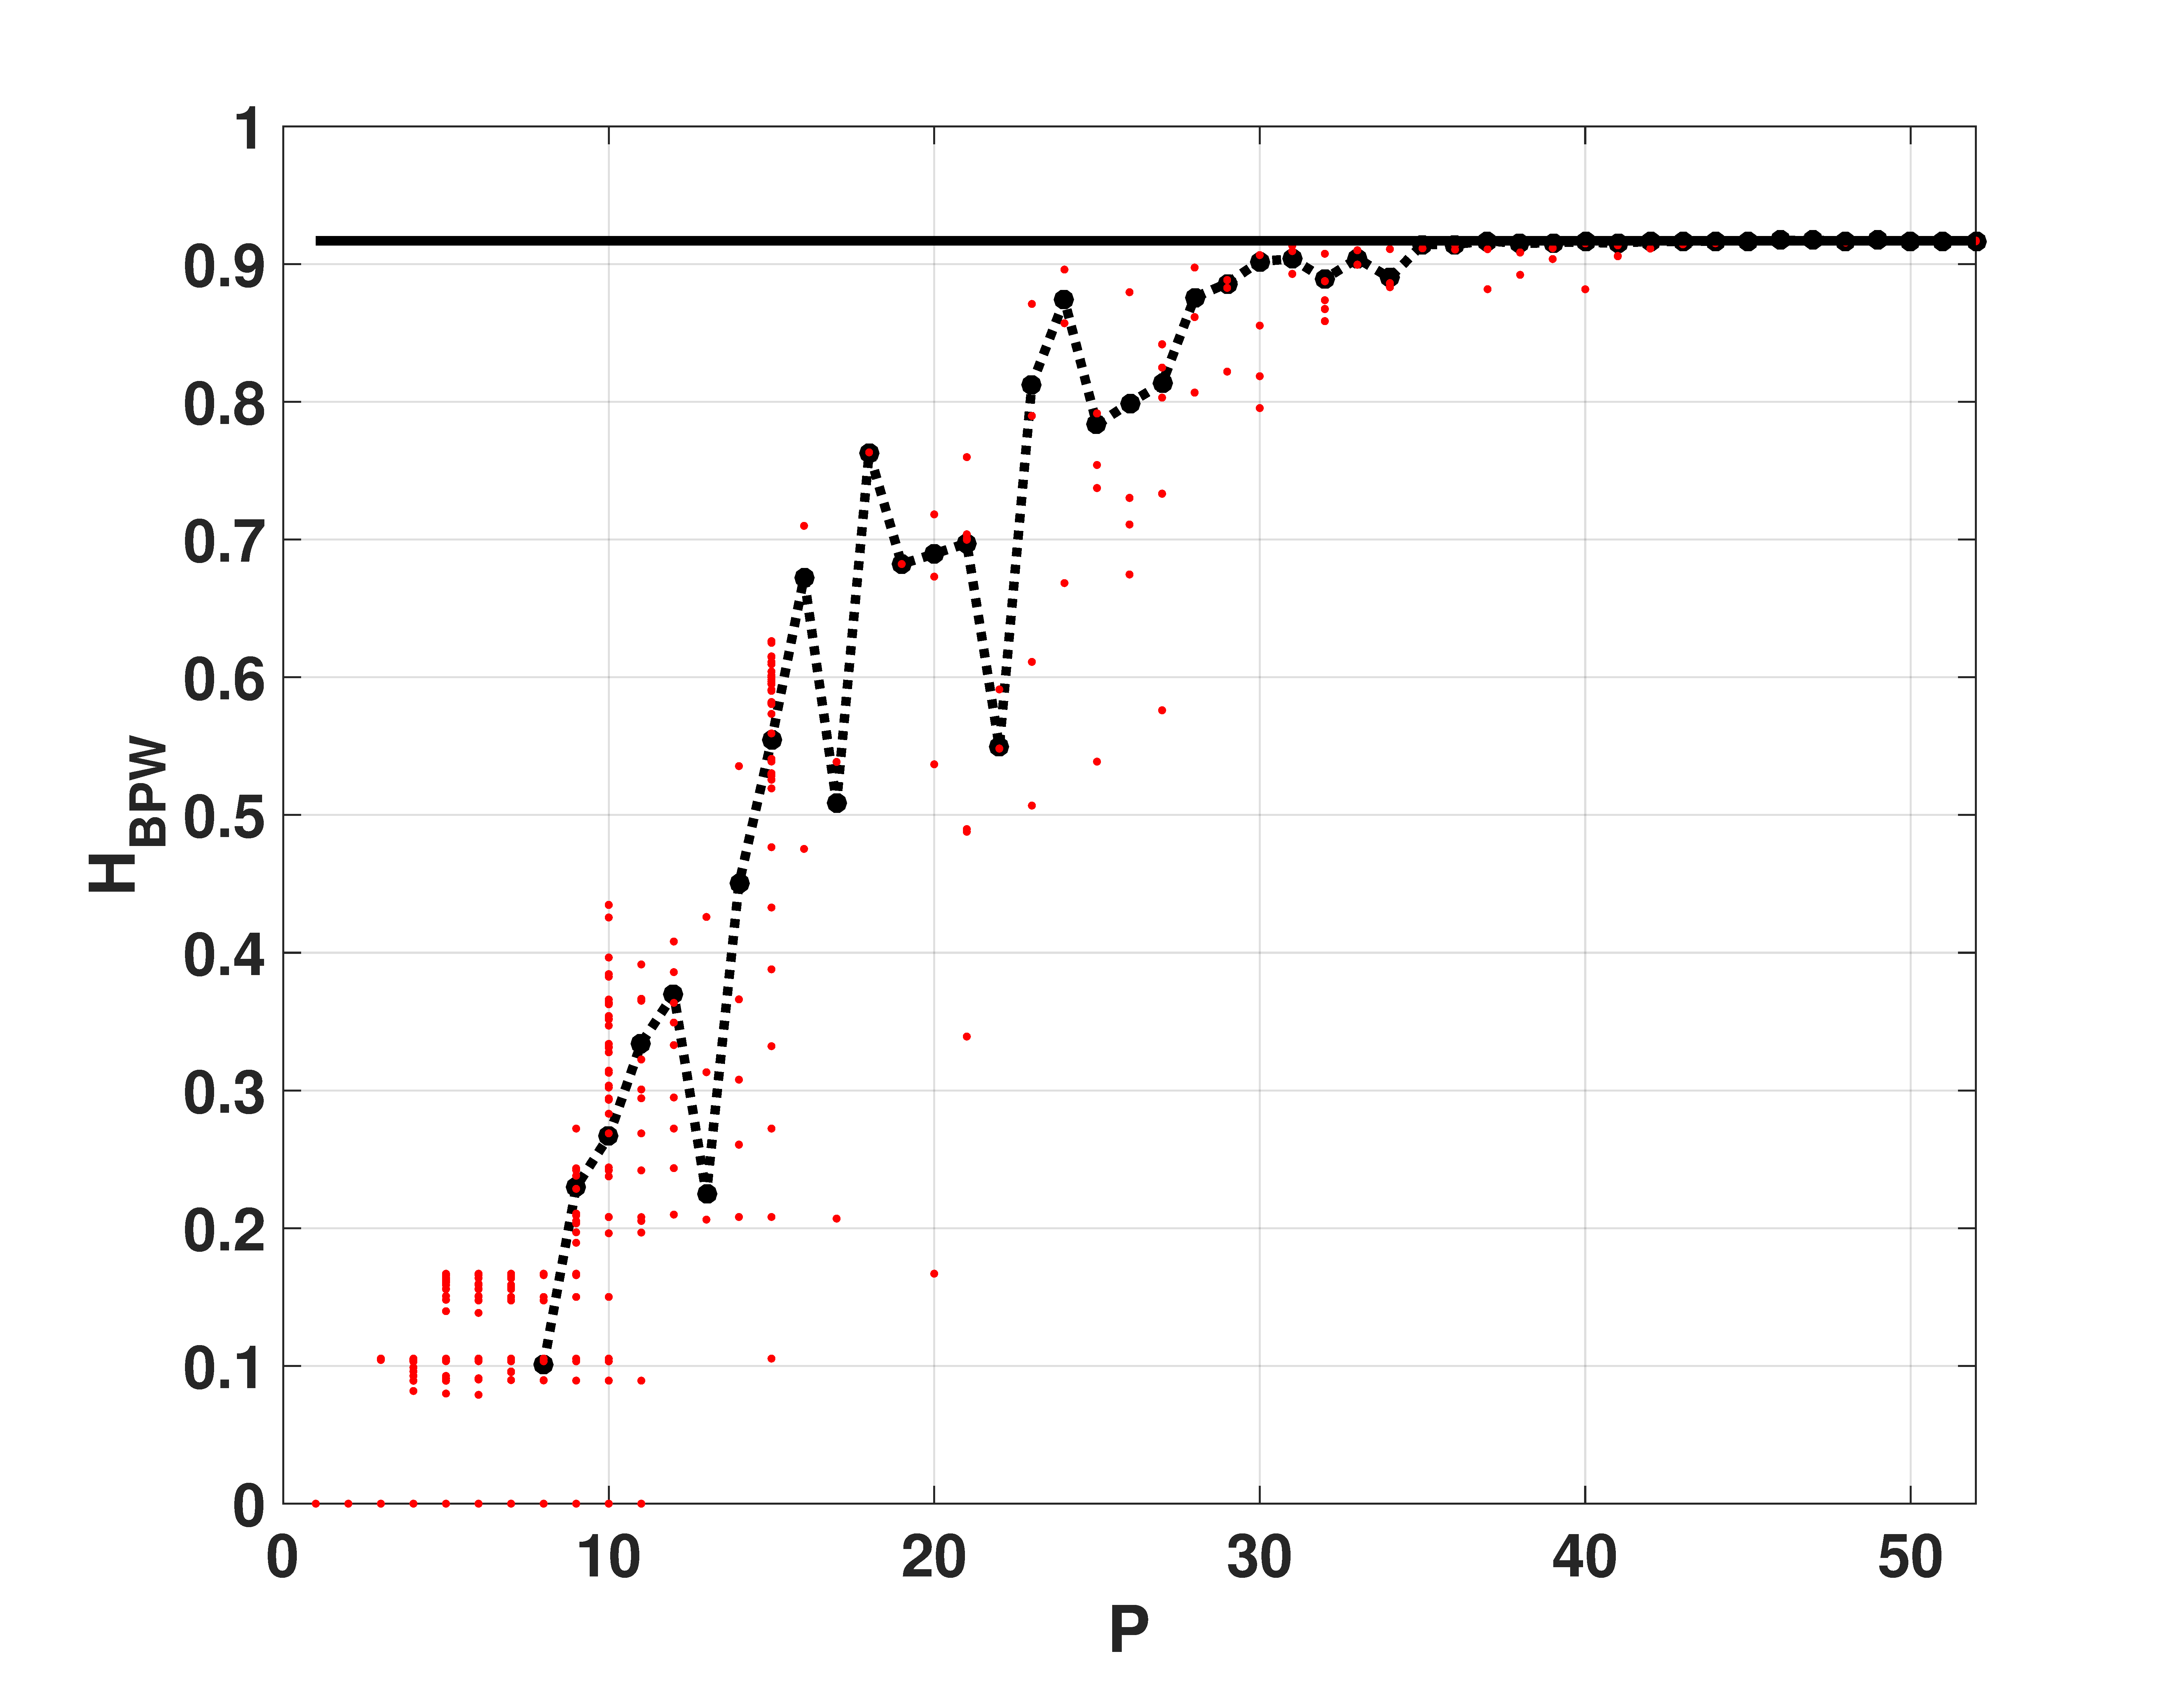
\includegraphics[width=.49\textwidth]{Hbpw_Odd}
	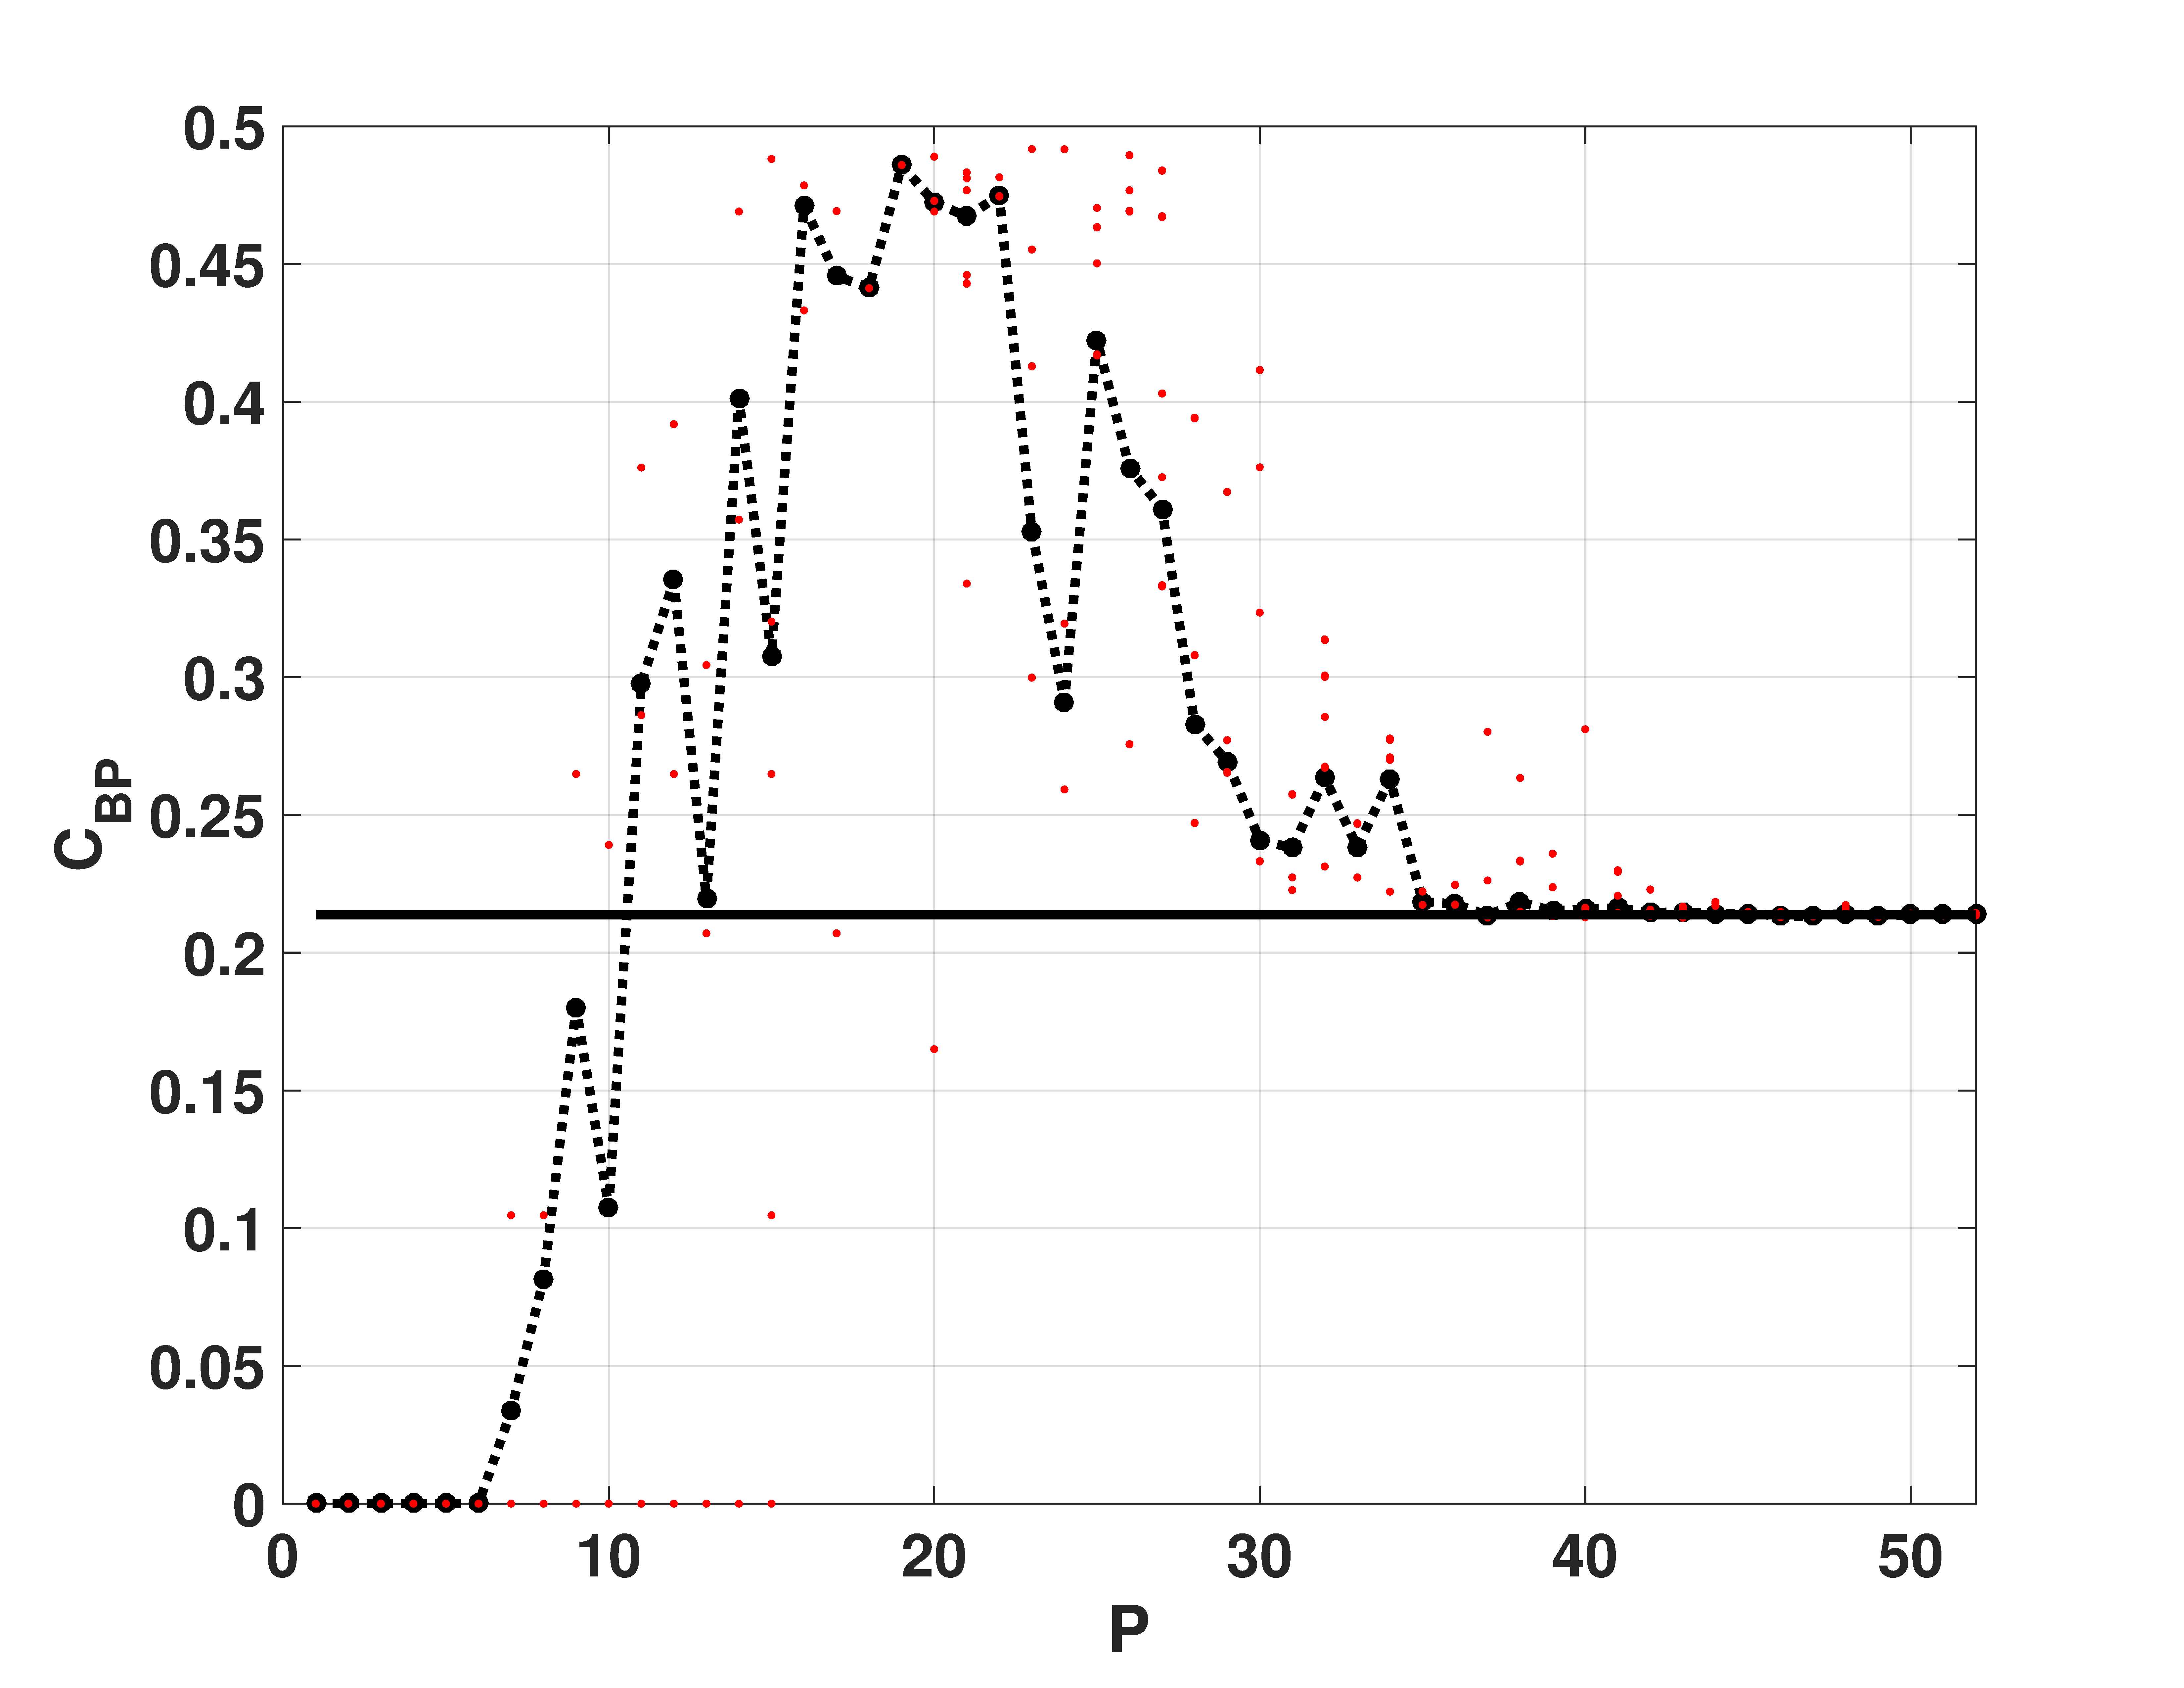
\includegraphics[width=.49\textwidth]{Cbp_Odd}
	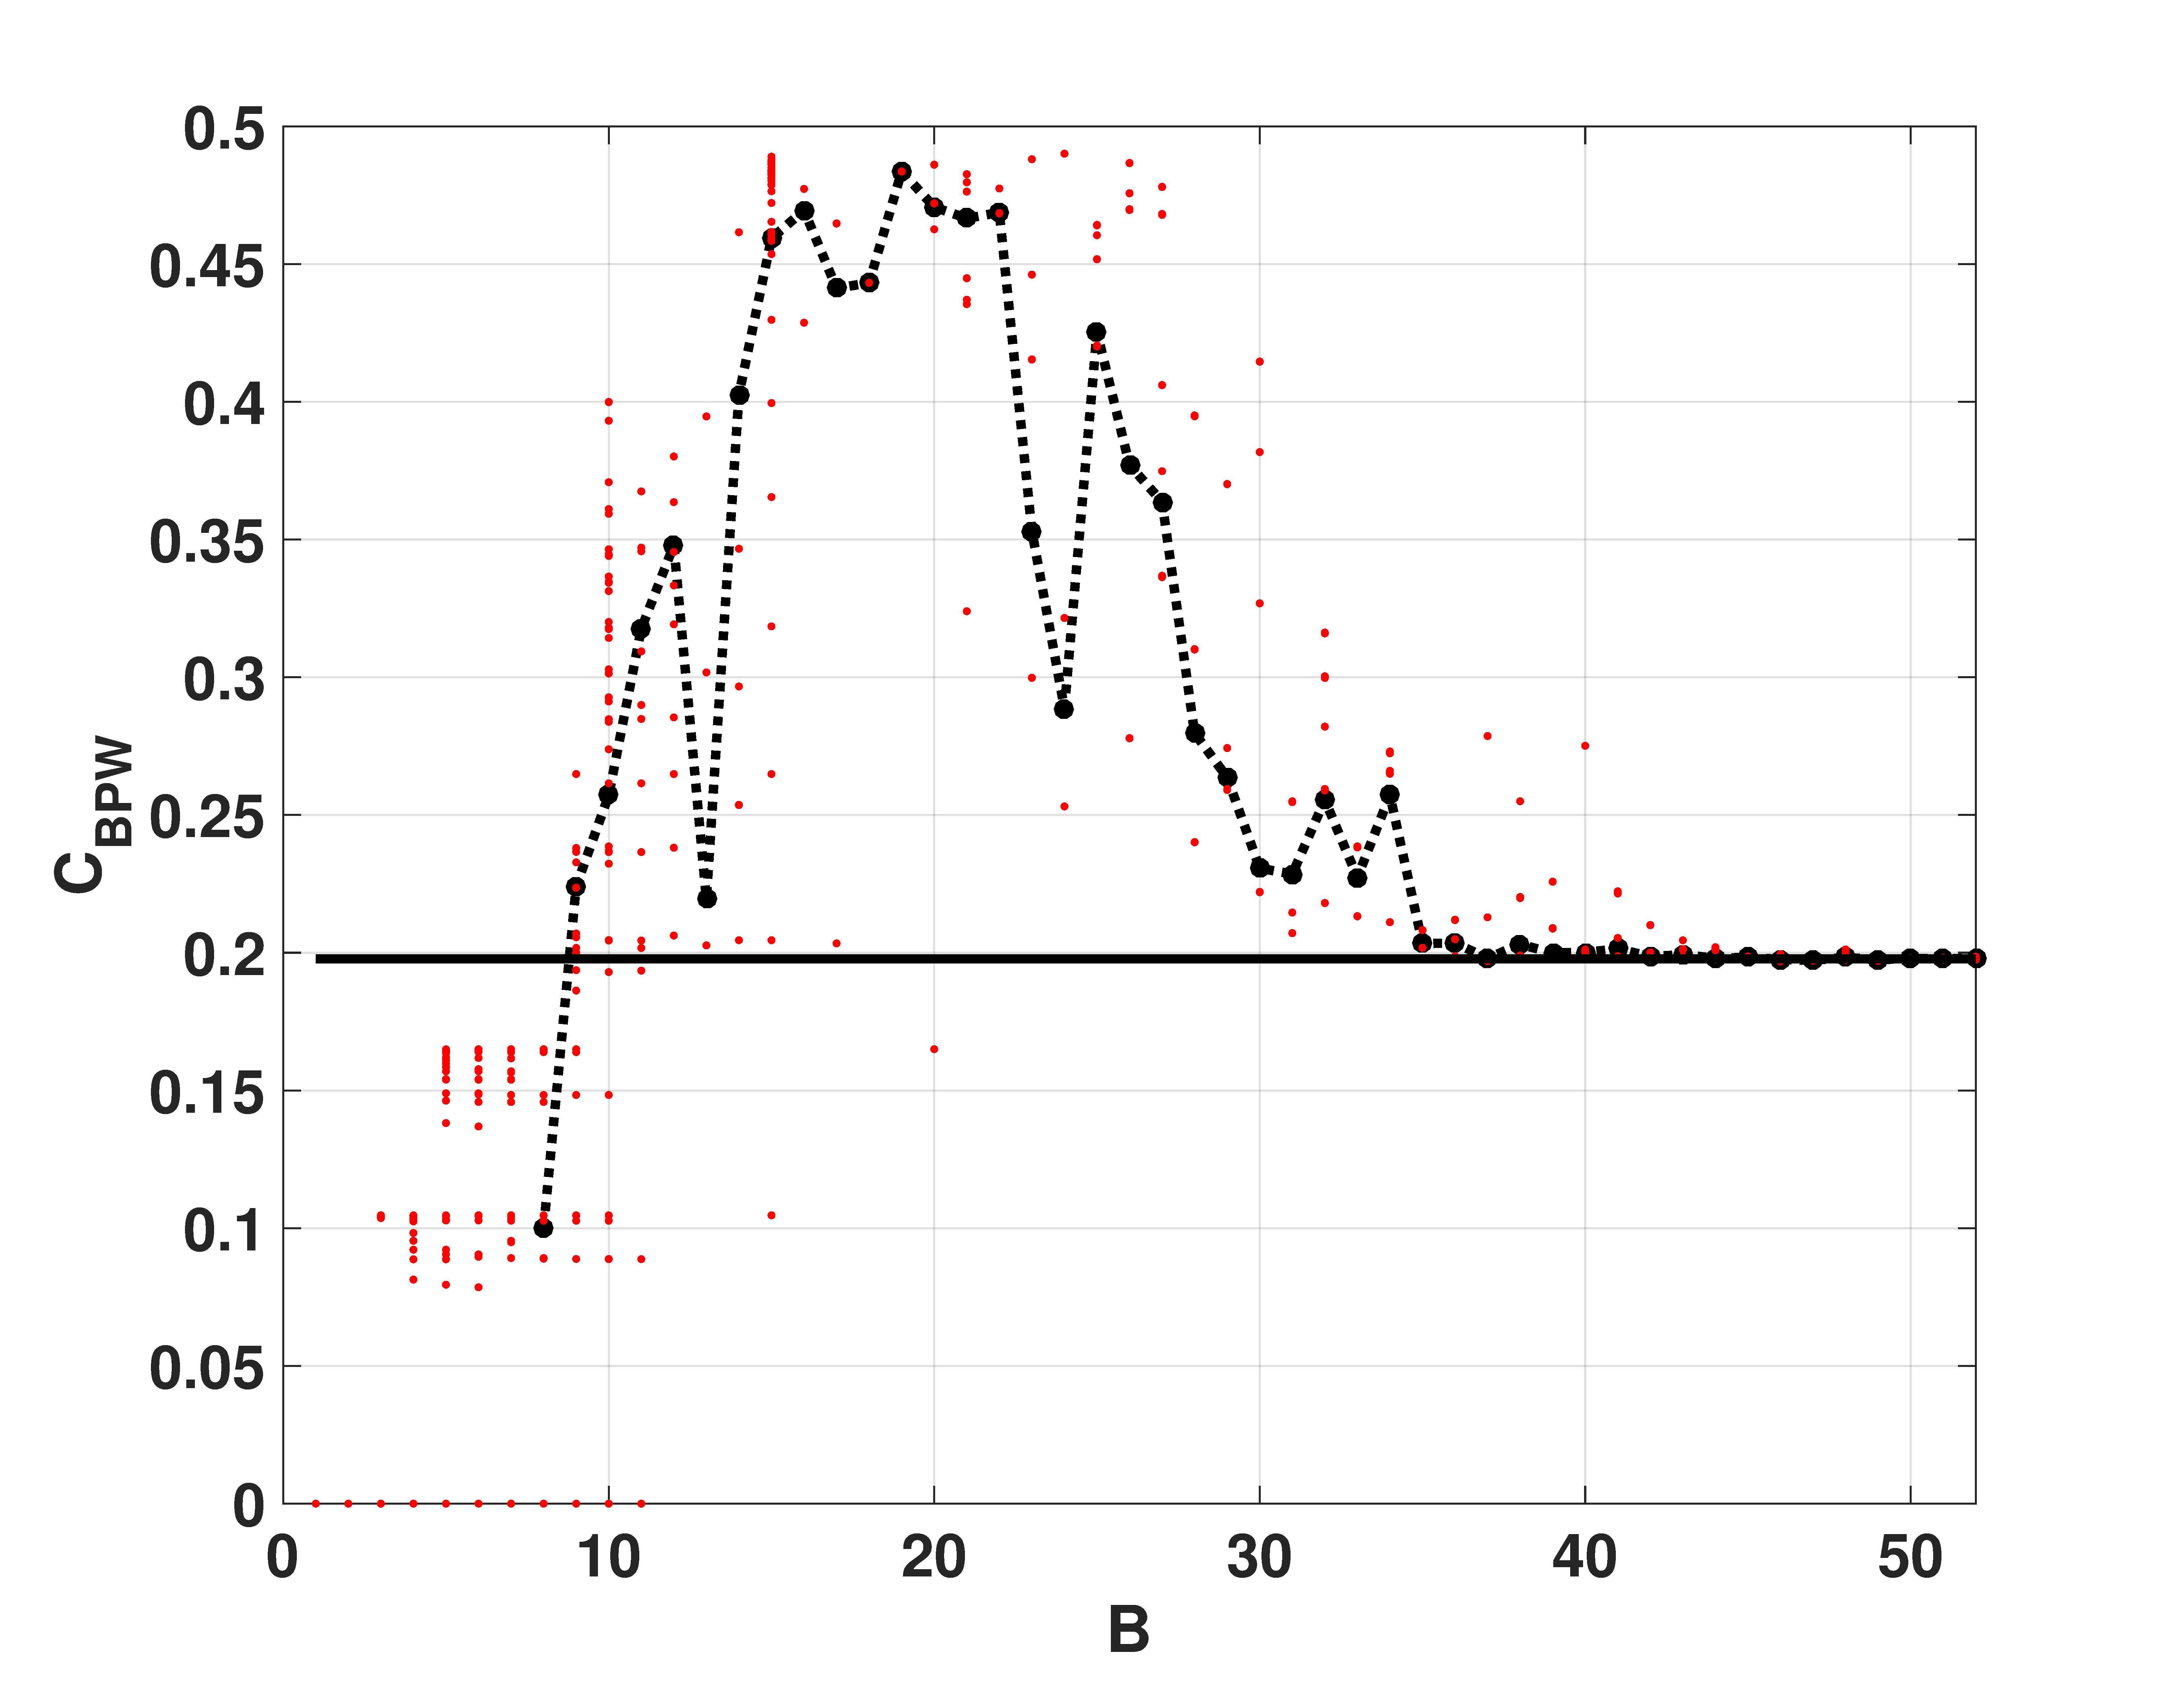
\includegraphics[width=.49\textwidth]{Cbpw_Odd}
	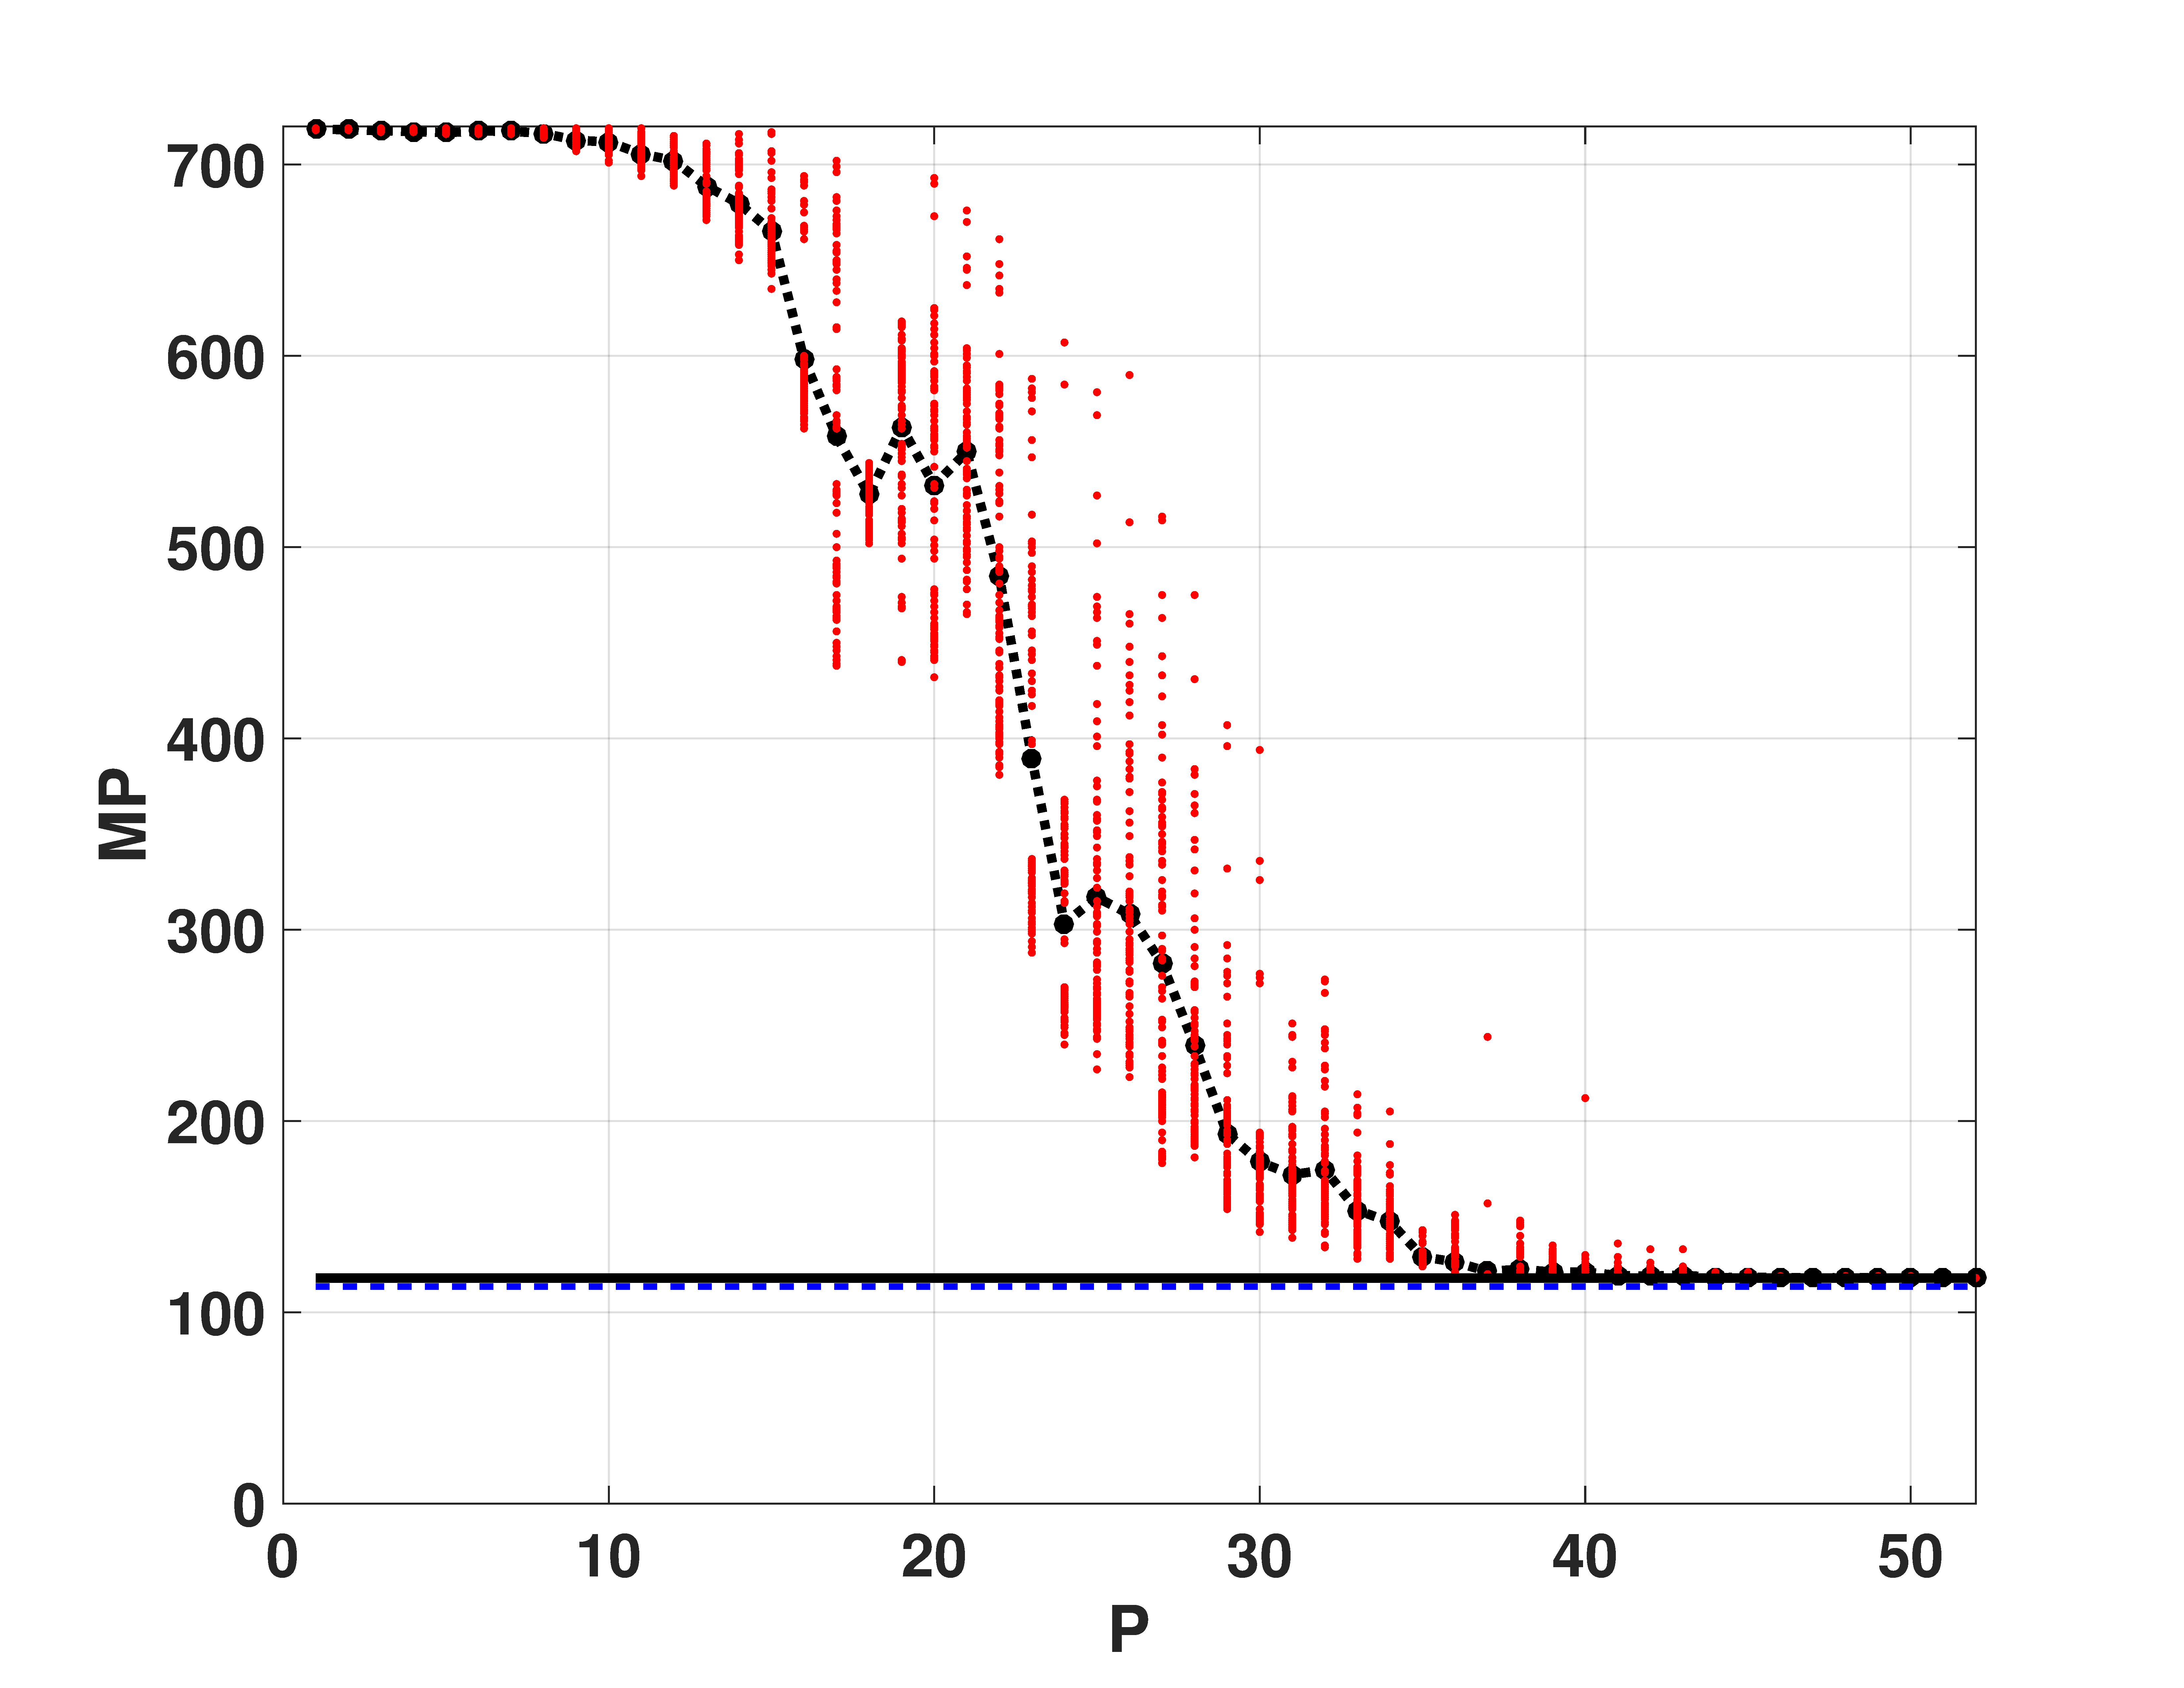
\includegraphics[width=.49\textwidth]{MP_Odd}
	\caption{Statistical properties of the ODD map: (a) $H_{val}$ vs $B$ (b) $H_{BP}$ vs $B$ (c) $C_{BP}$ vs $B$ (d) $MP$ vs $B$.}
	\label{fig:ODD_QuantiB}
	\end{figure}

\textcolor{red}{FALTA VER PLANOS DOBLE ENTROPÍA}

\begin{figure}
	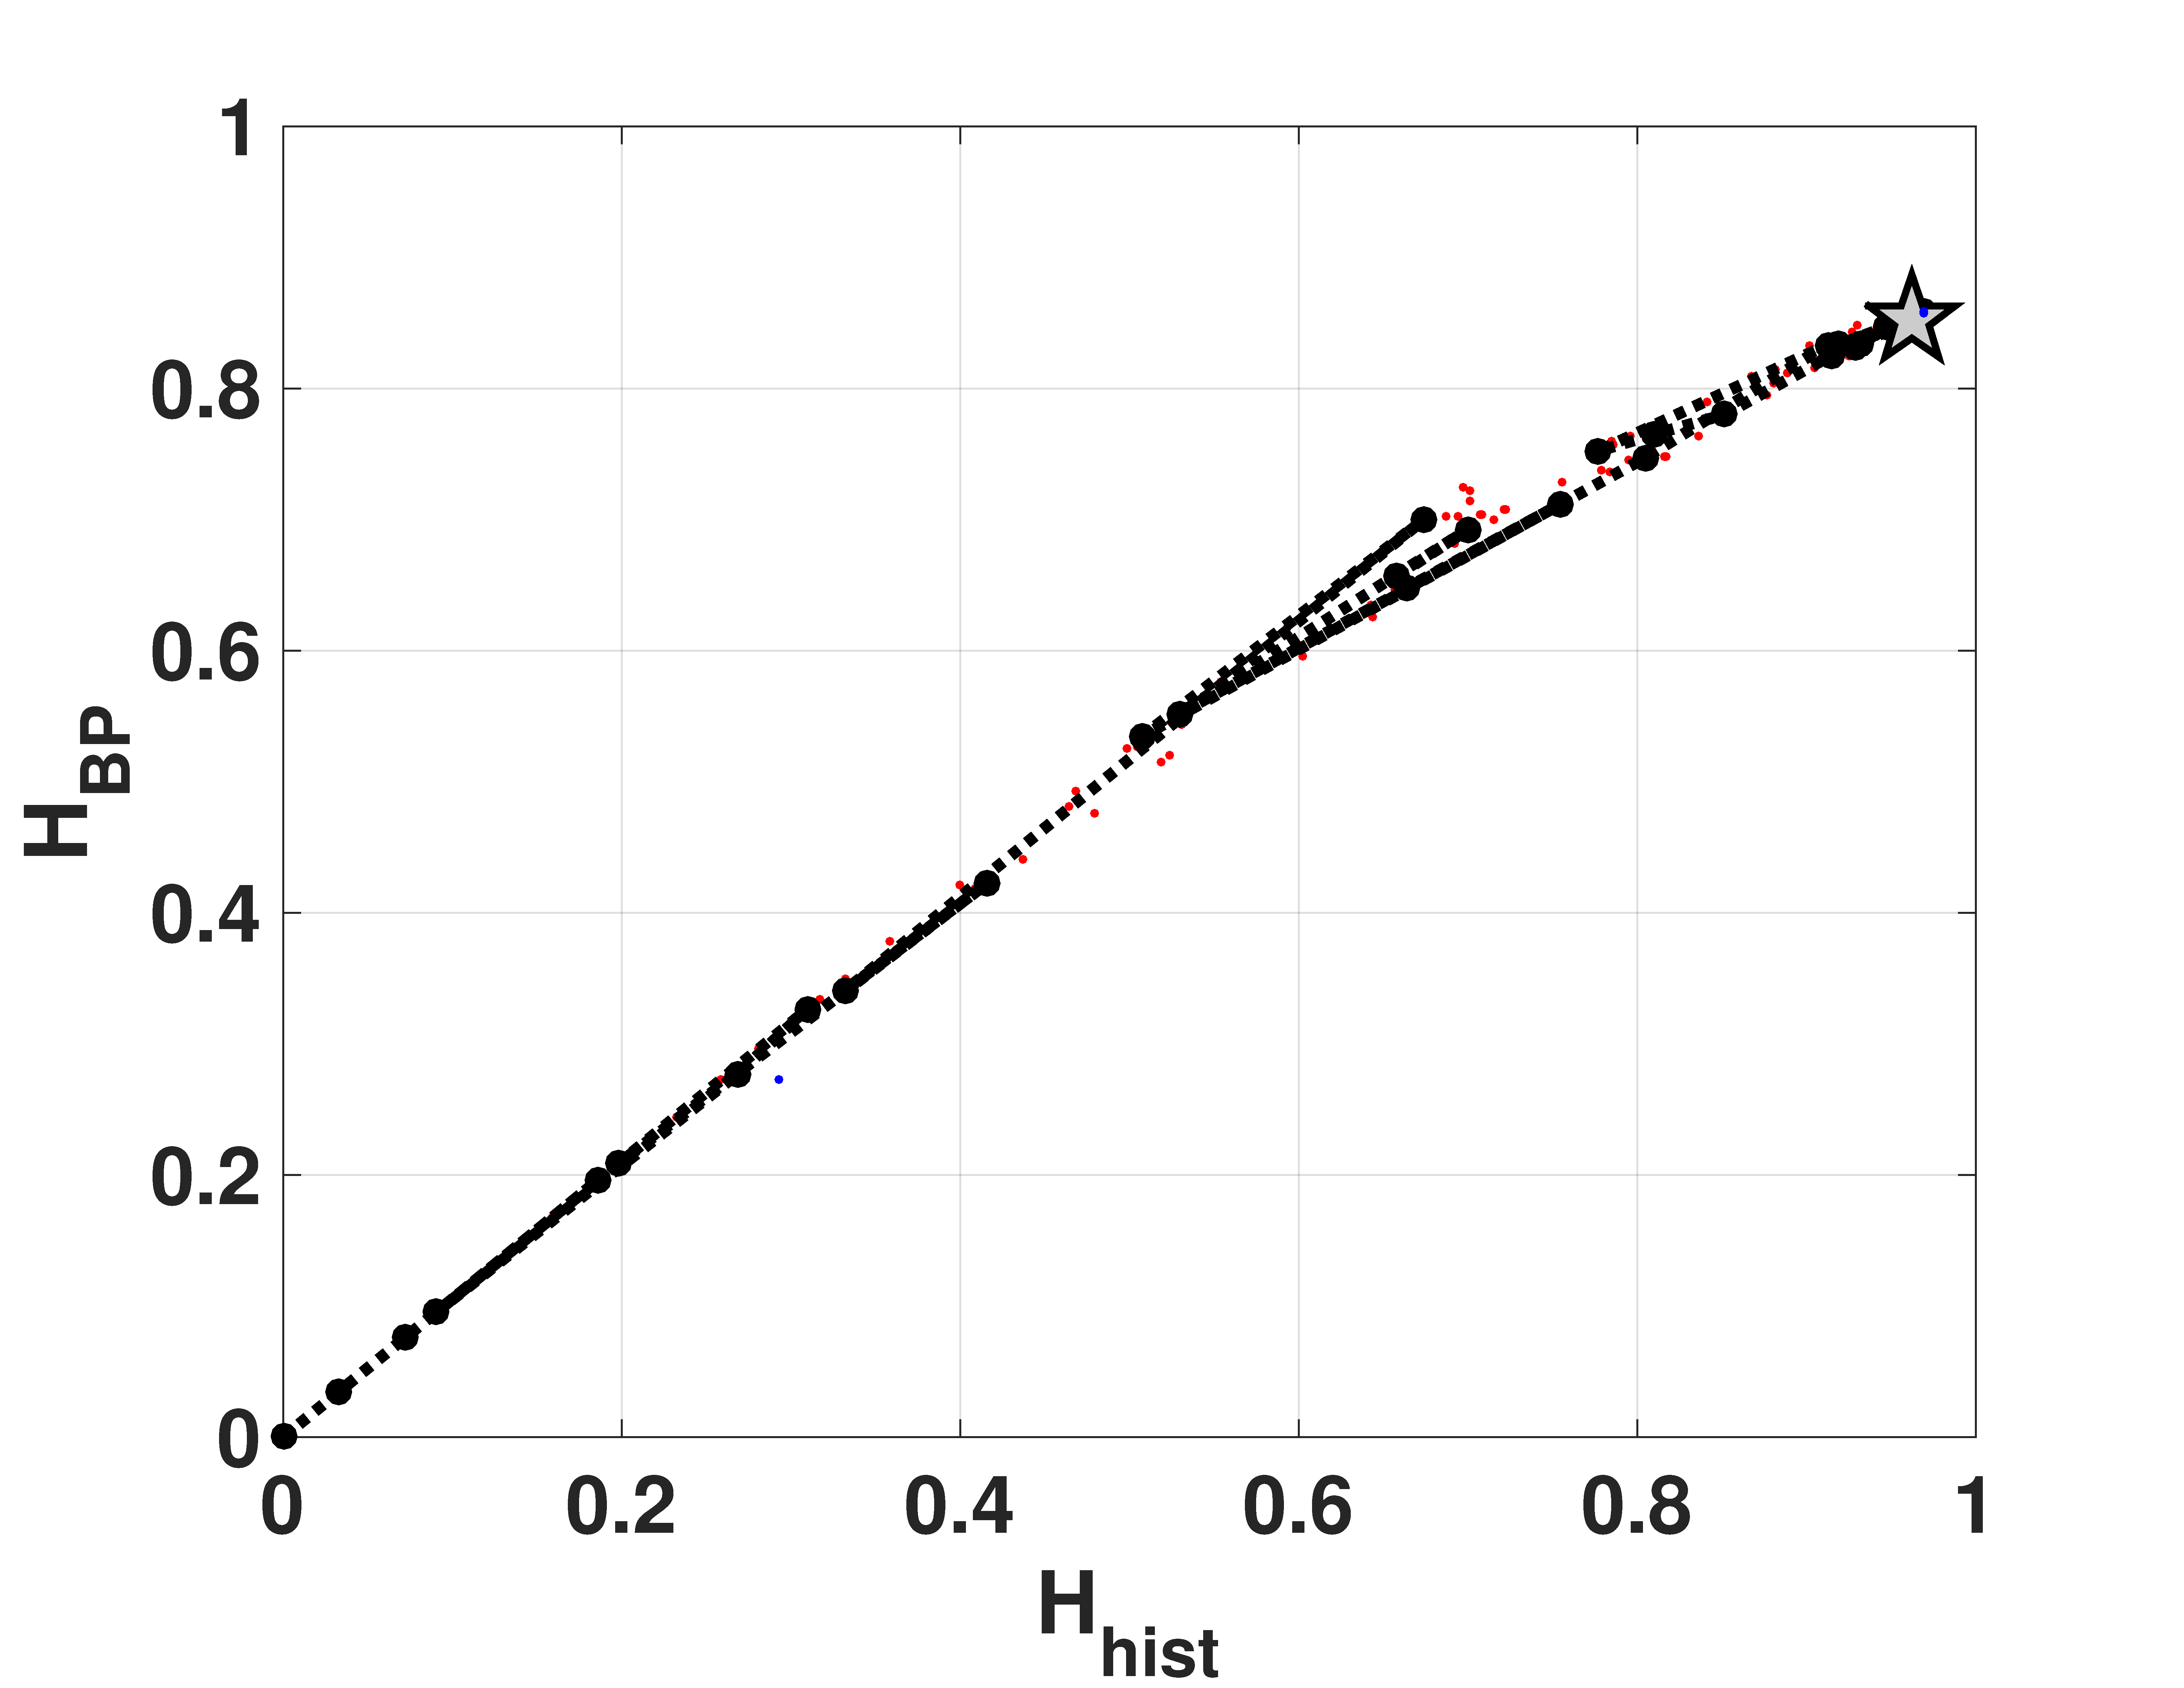
\includegraphics[width=.49\textwidth]{HbpHval_Even}
	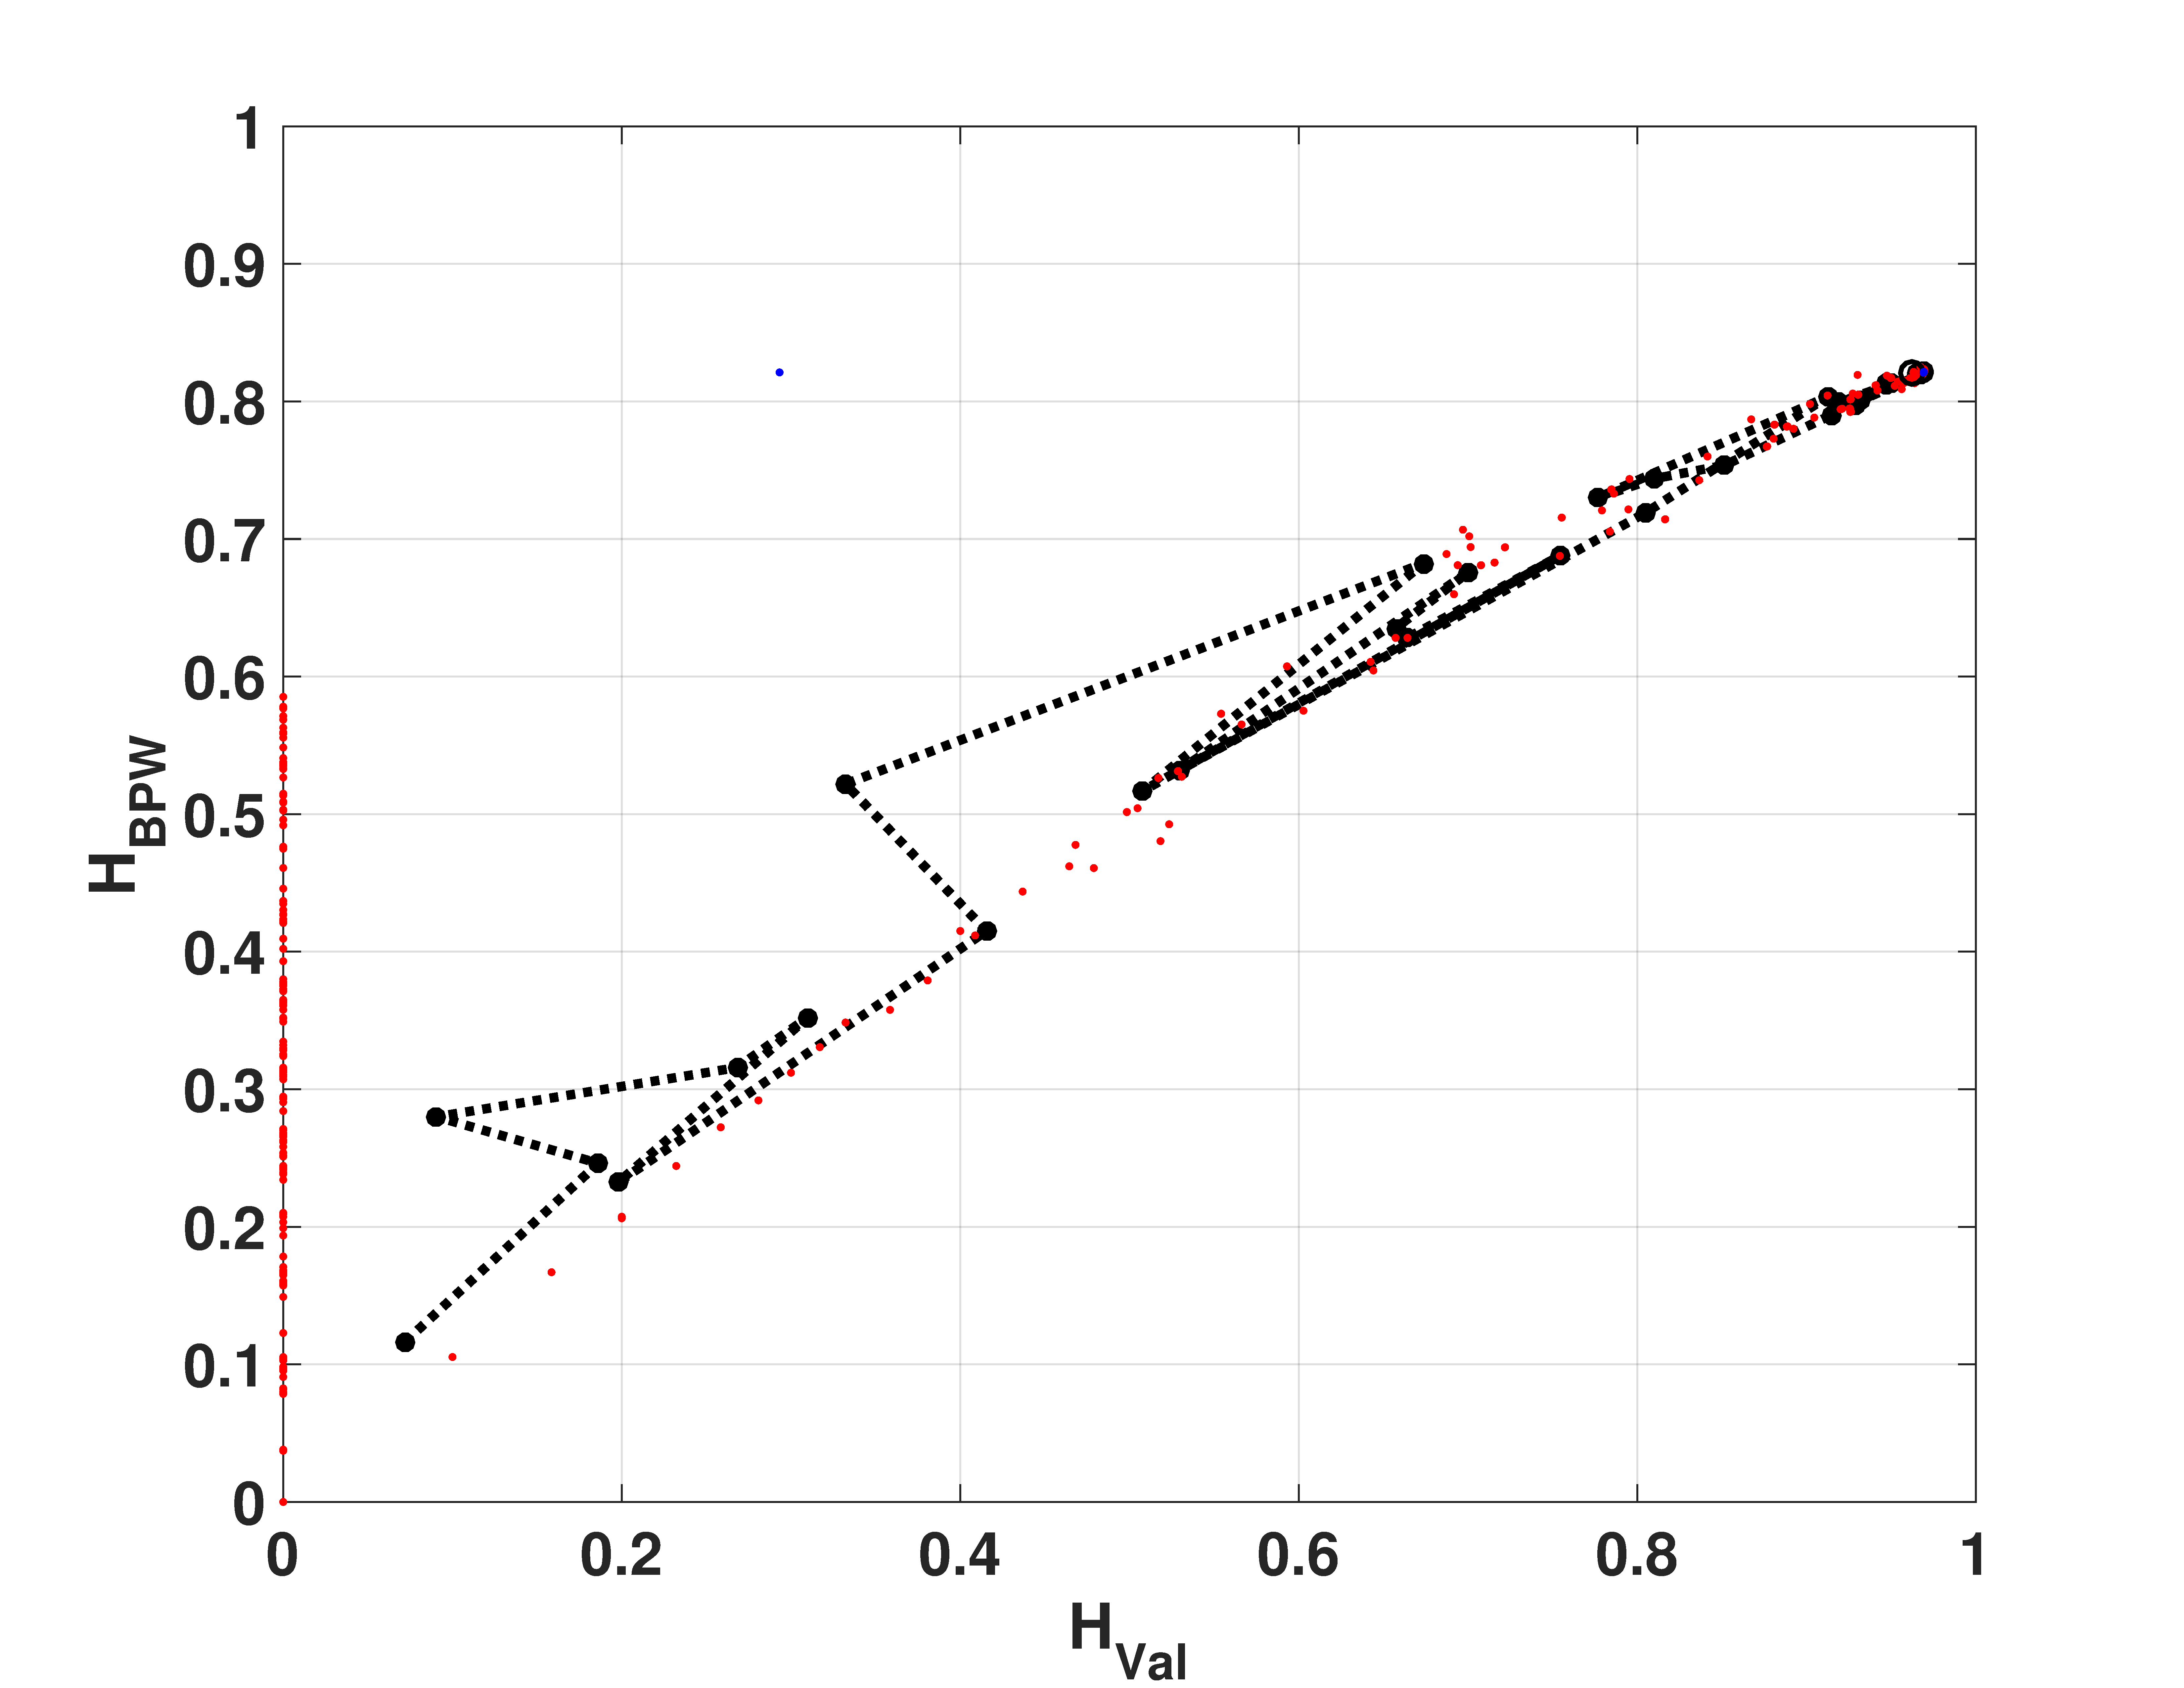
\includegraphics[width=.49\textwidth]{HbpwHval_Even}
	\caption{Evolution of statistical properties in double entropy plane of EVEN map: (a) $H_{val}$ vs $H_{BP}$ (b) $H_{val}$ vs $H_{BPW}$.}
	\label{fig:EVEN_HH}
\end{figure}

\begin{figure}
	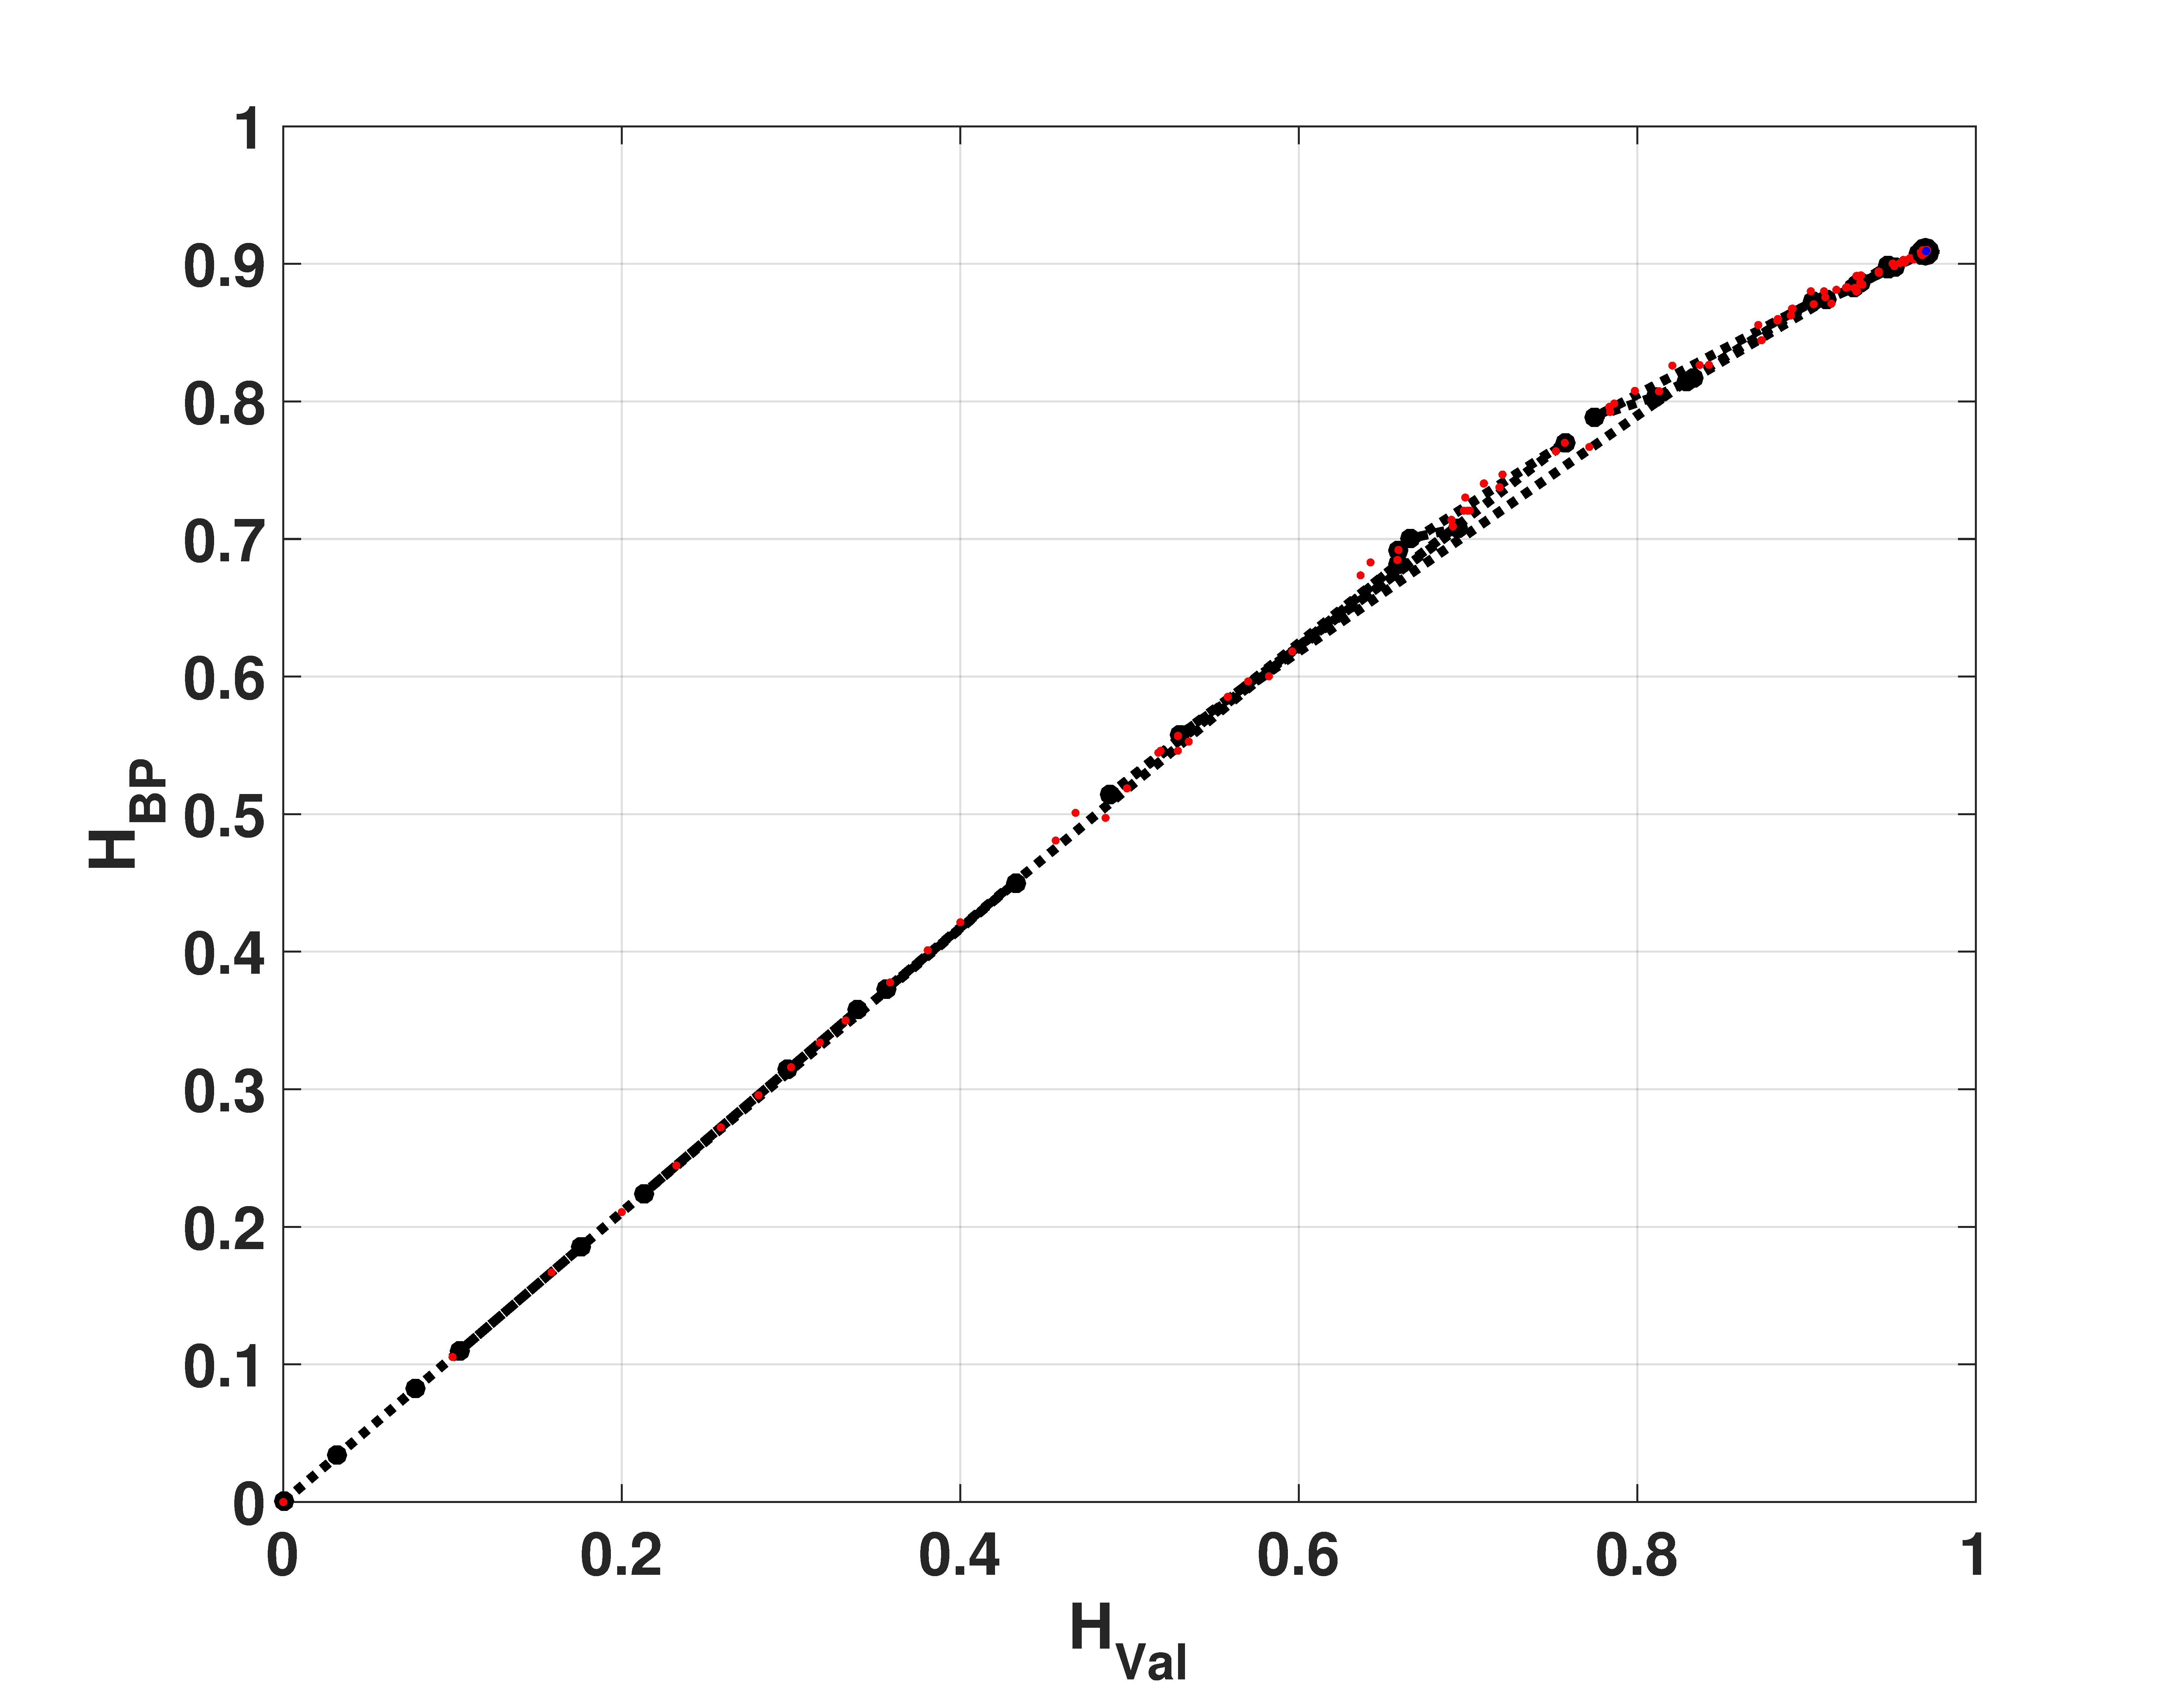
\includegraphics[width=.49\textwidth]{HbpHval_Odd}
	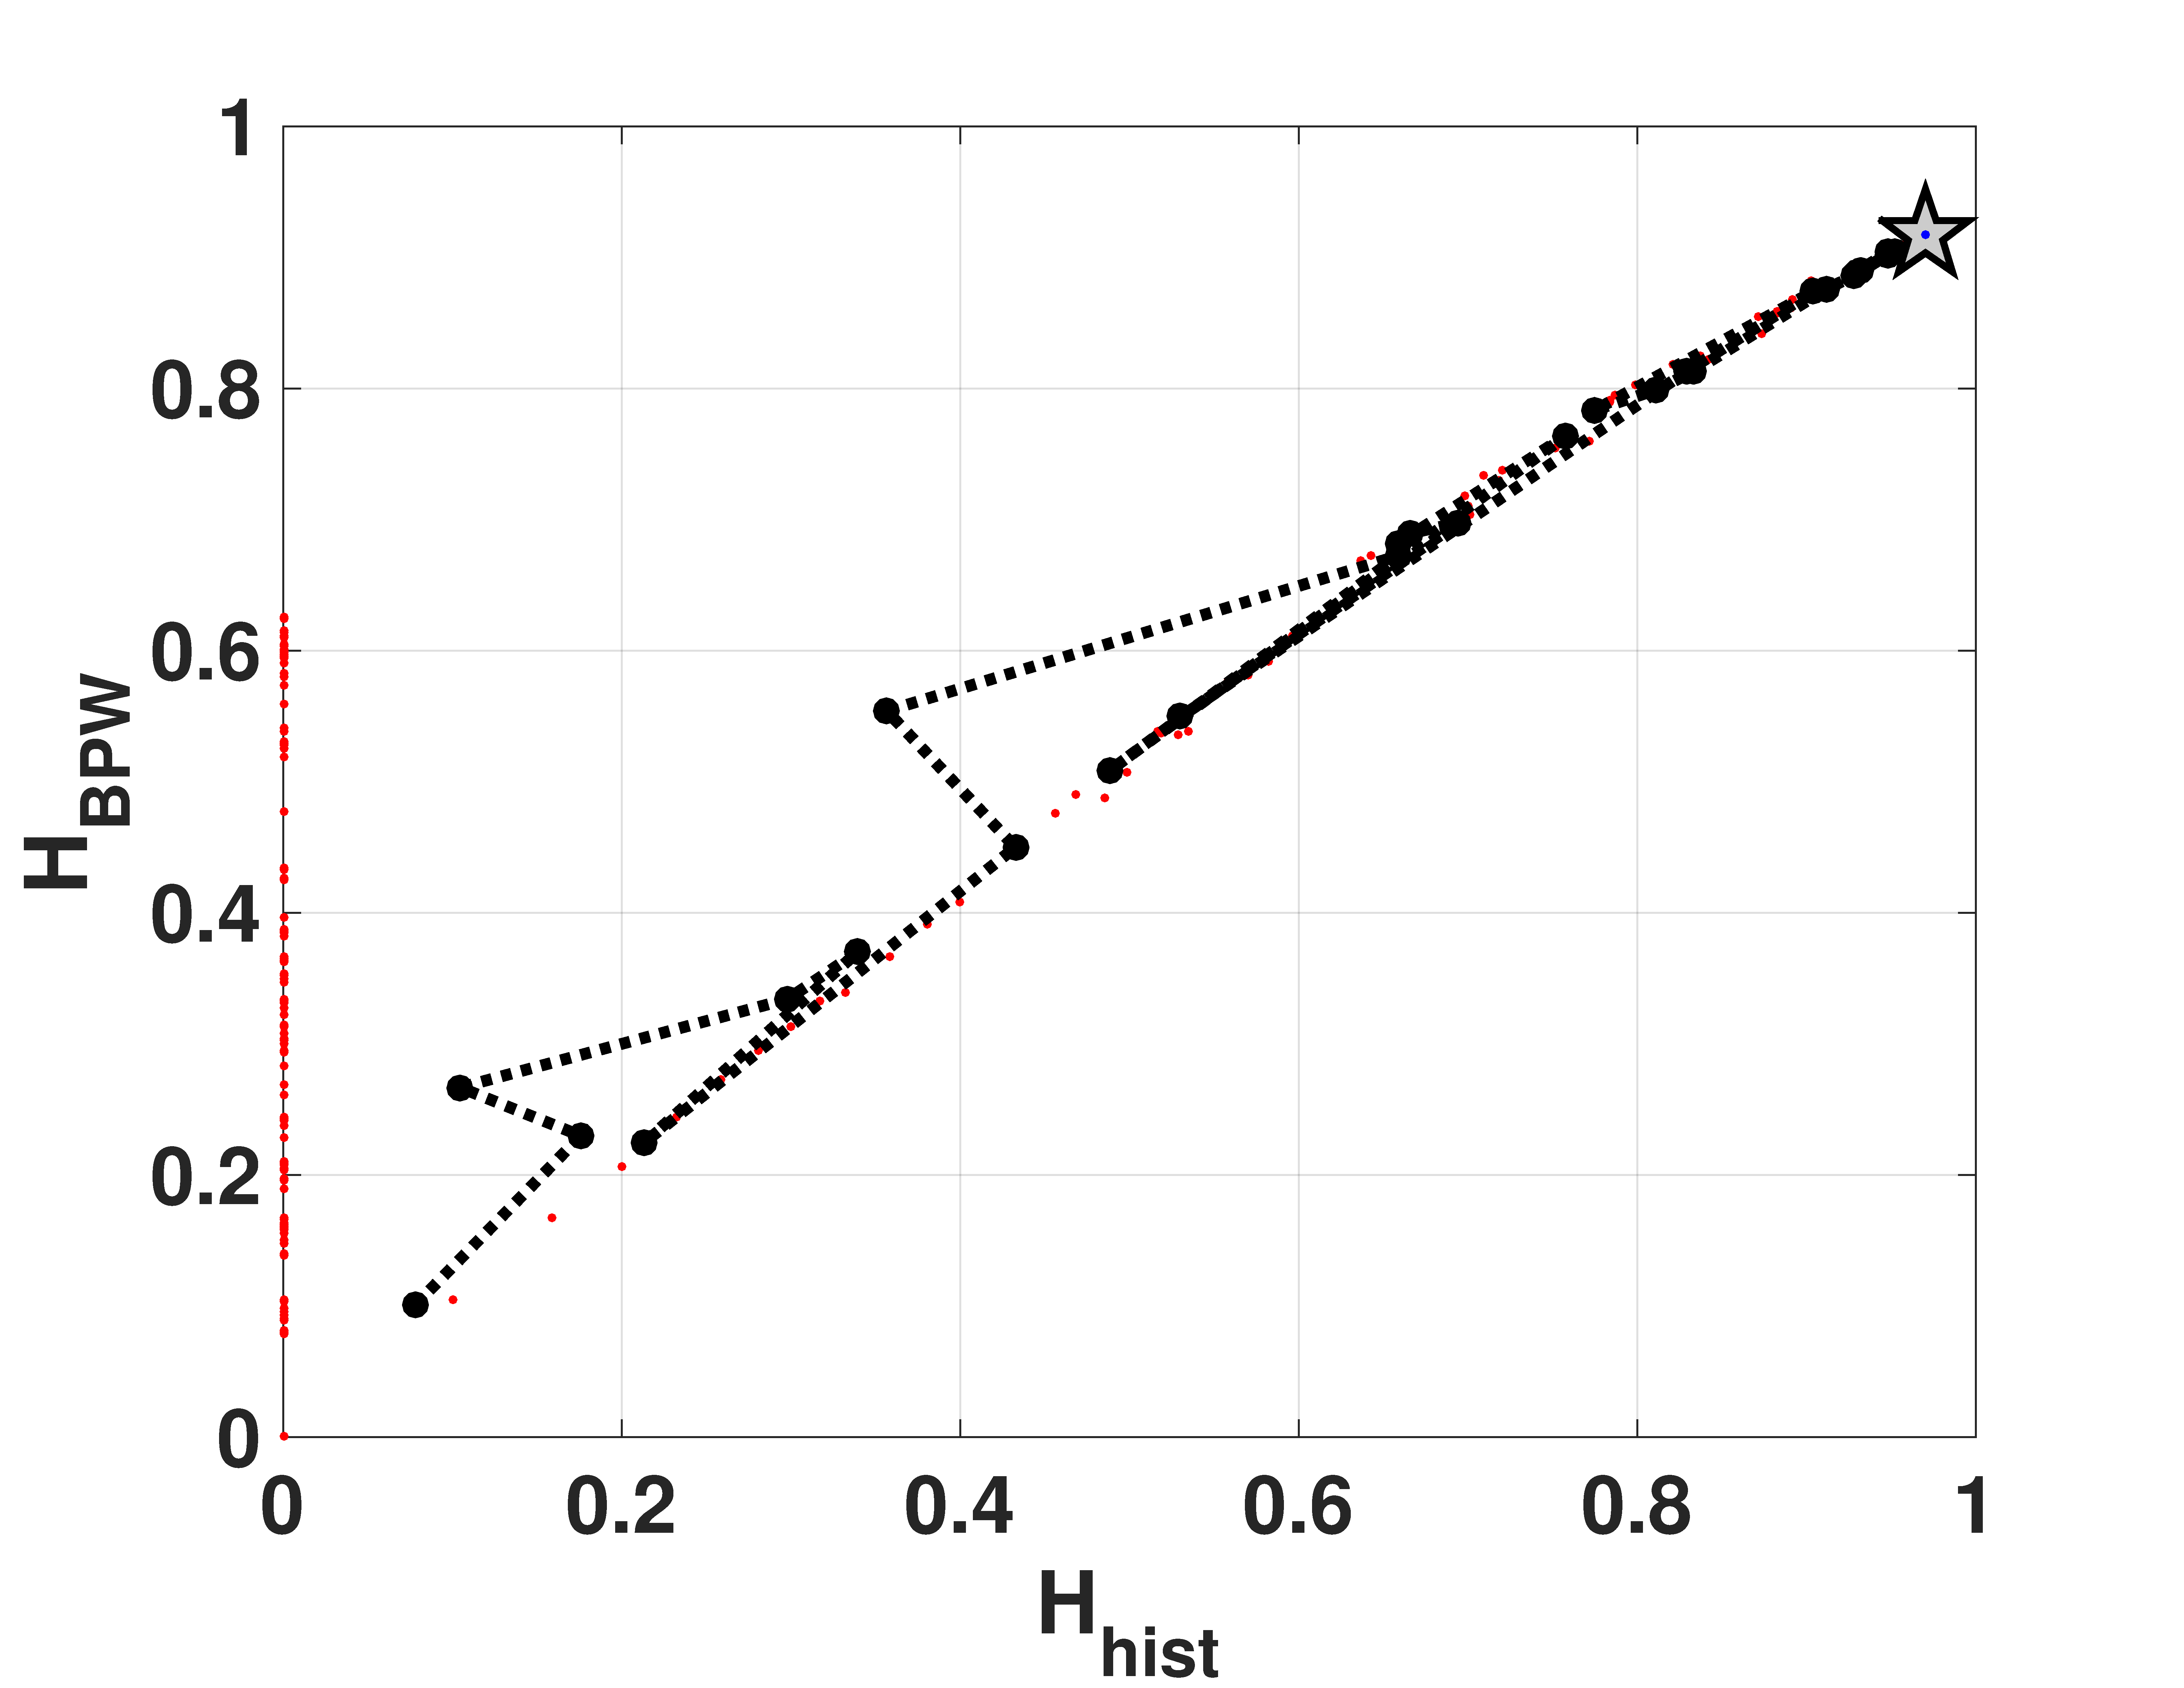
\includegraphics[width=.49\textwidth]{HbpwHval_Odd}
	\caption{Evolution of statistical properties in double entropy plane of ODD map: (a) $H_{val}$ vs $H_{BP}$ (b) $H_{val}$ vs $H_{BPW}$.}
	\label{fig:ODD_HH}
\end{figure}

\textcolor{red}{FALTA VER PLANOS ENTROPÍA-COMPLEJIDAD}

\begin{figure}
	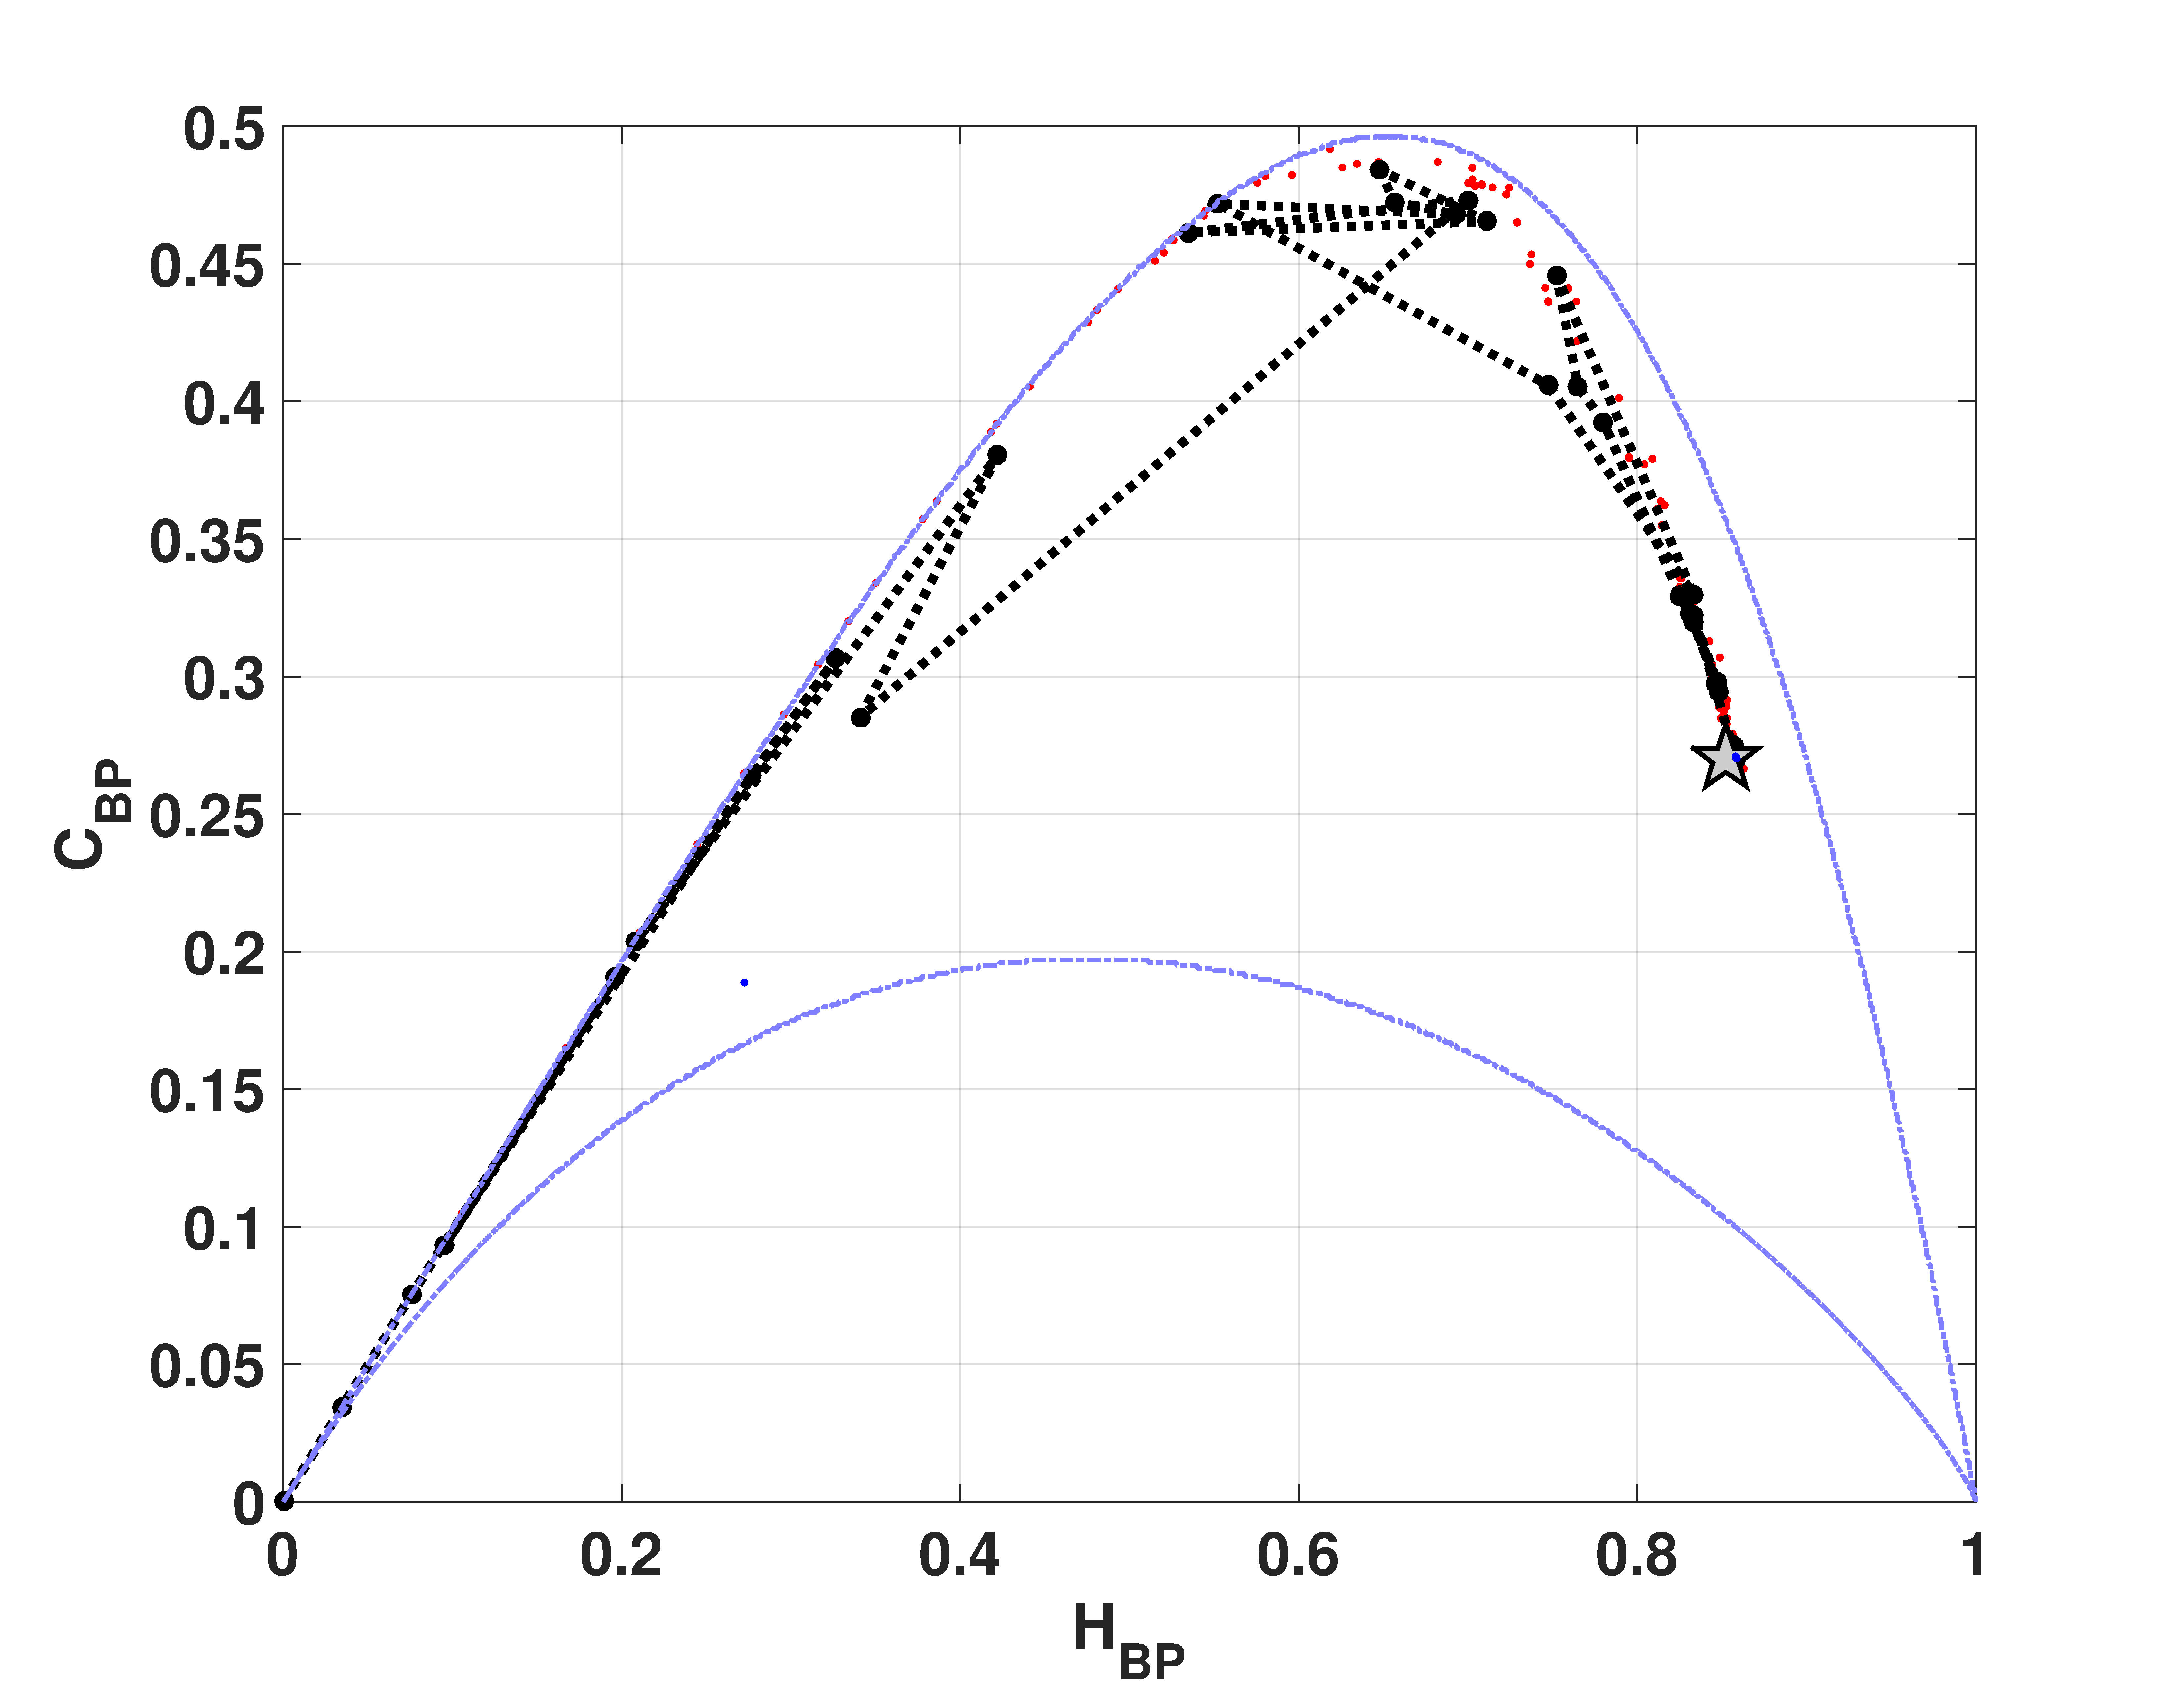
\includegraphics[width=.49\textwidth]{CbpHbp_Even}
	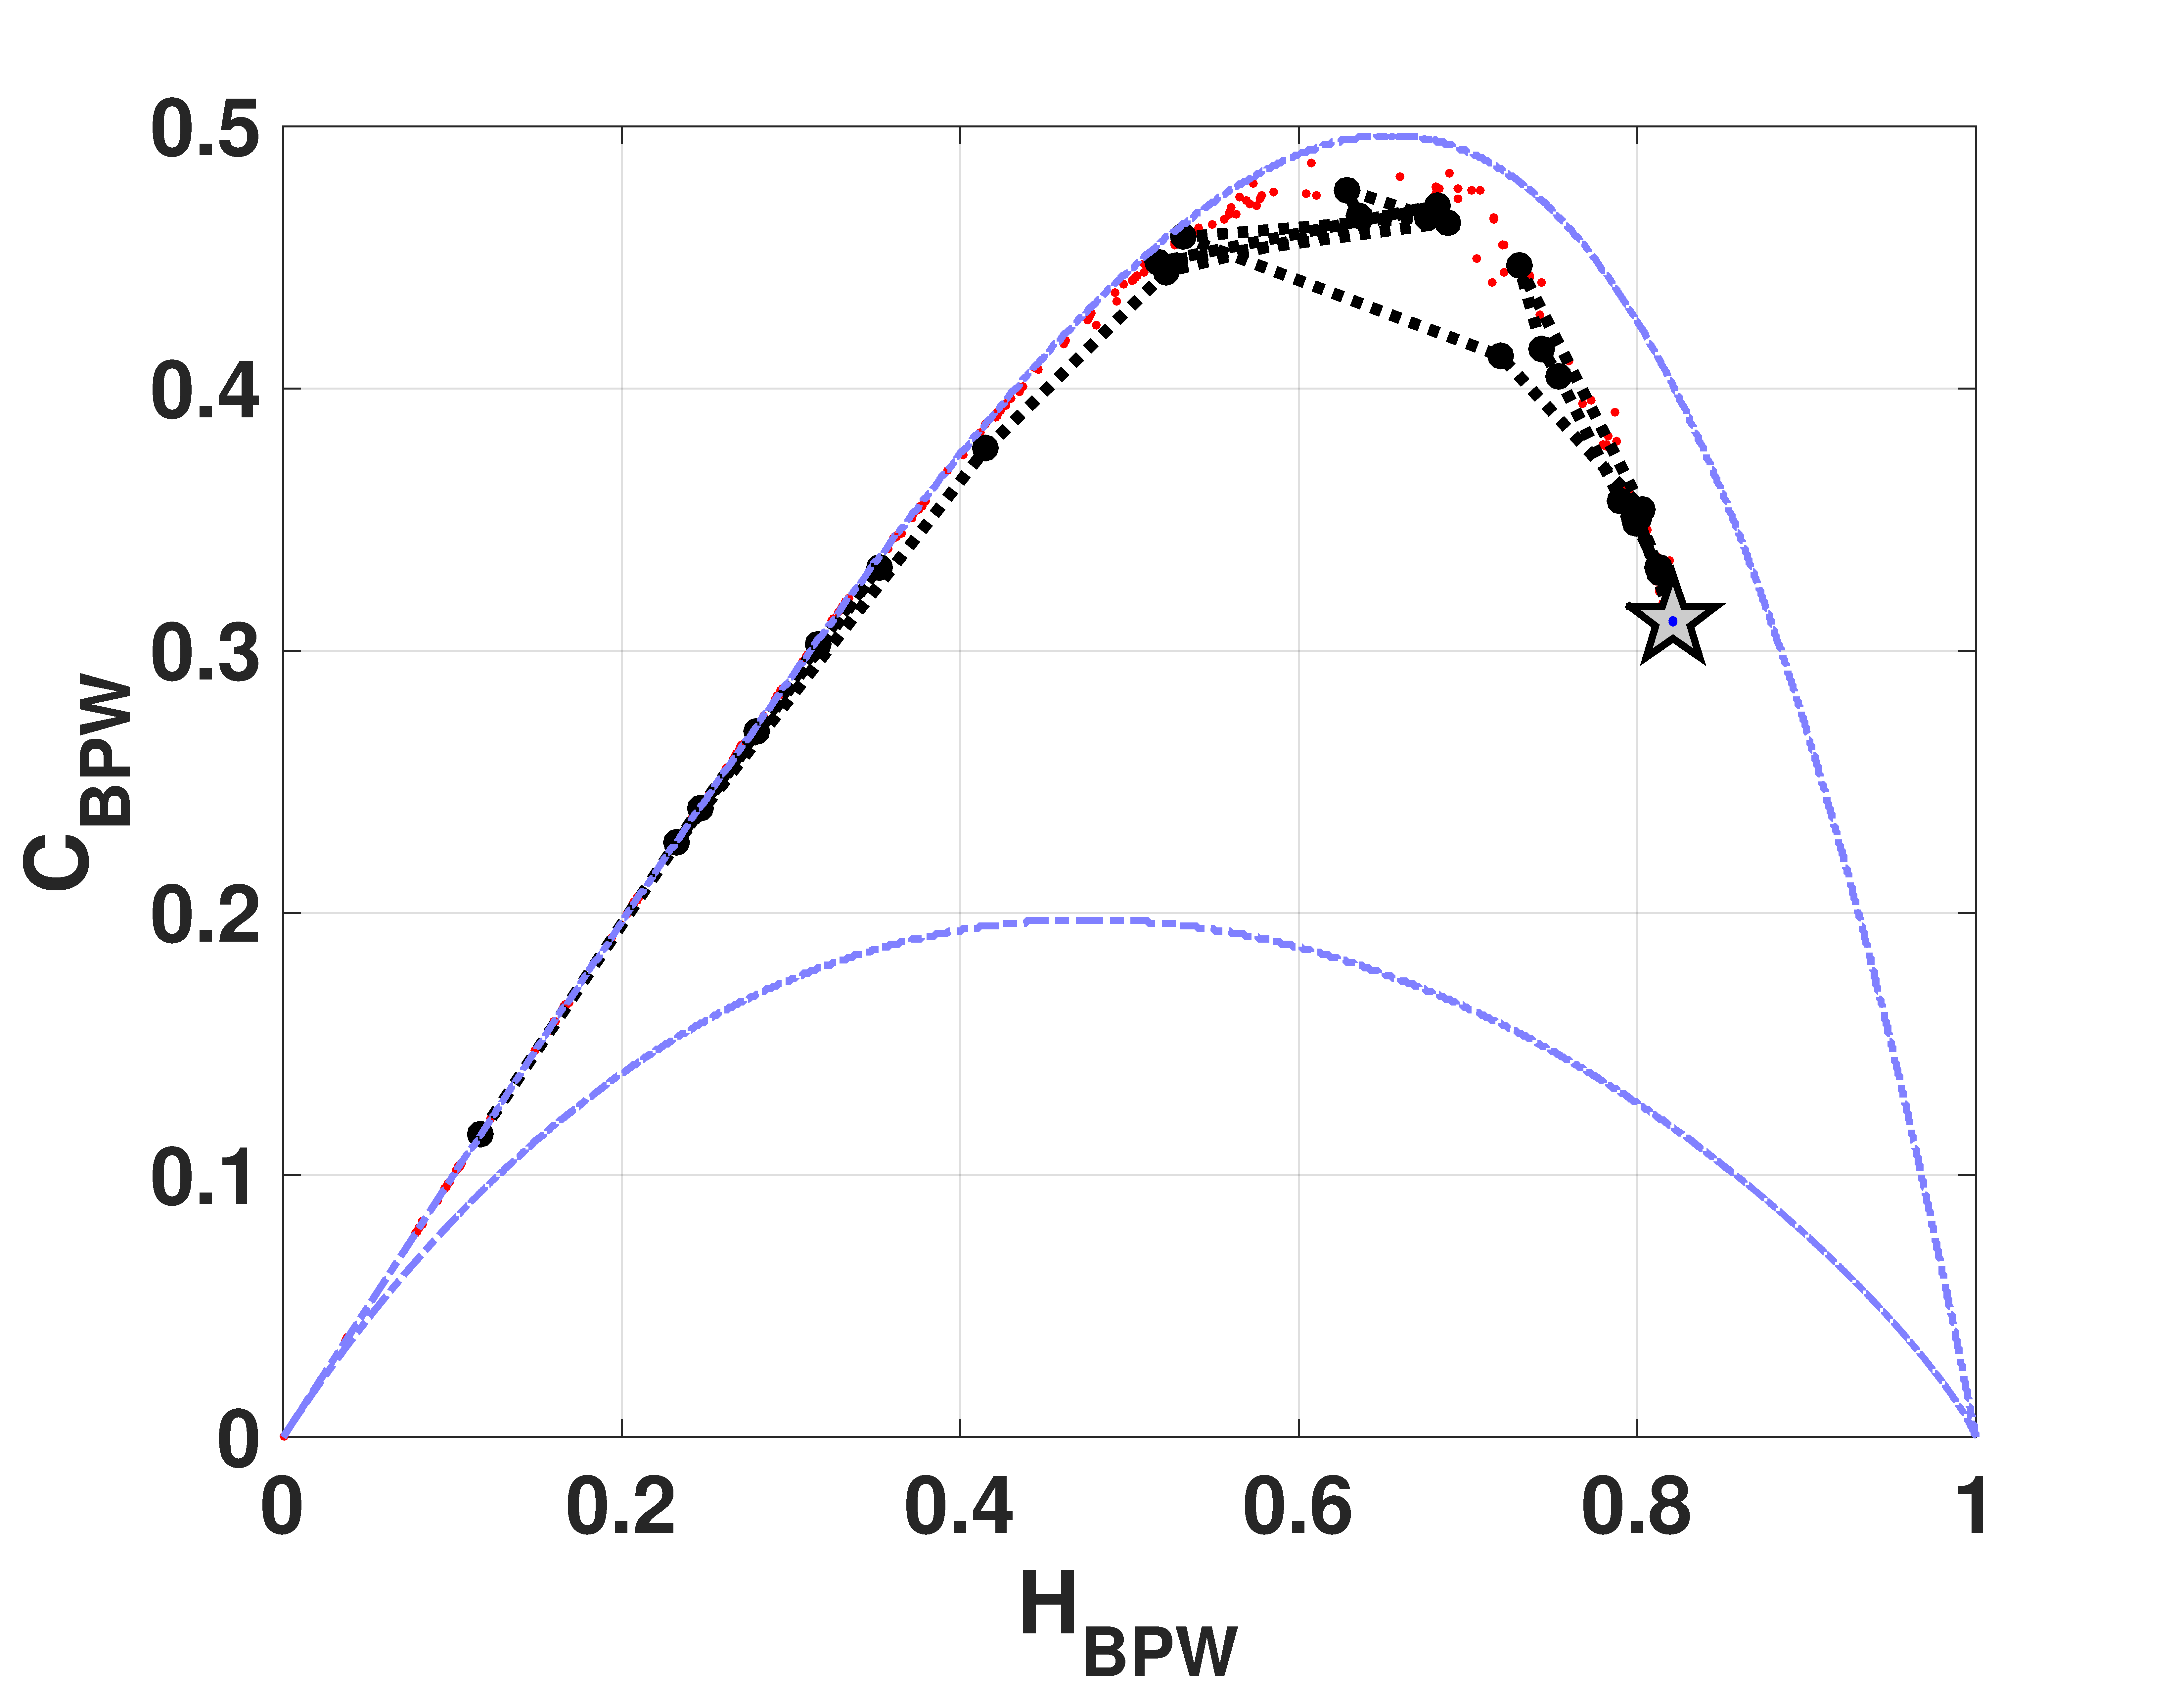
\includegraphics[width=.49\textwidth]{CbpwHbpw_Even}
	\caption{Evolution of statistical properties in entropy-complexity plane of EVEN map: (a) $C_{BP}$ vs $H_{BP}$ (b) $C_{BPW}$ vs $H_{BPW}$.}
	\label{fig:EVEN_HC}
\end{figure}

\begin{figure}
	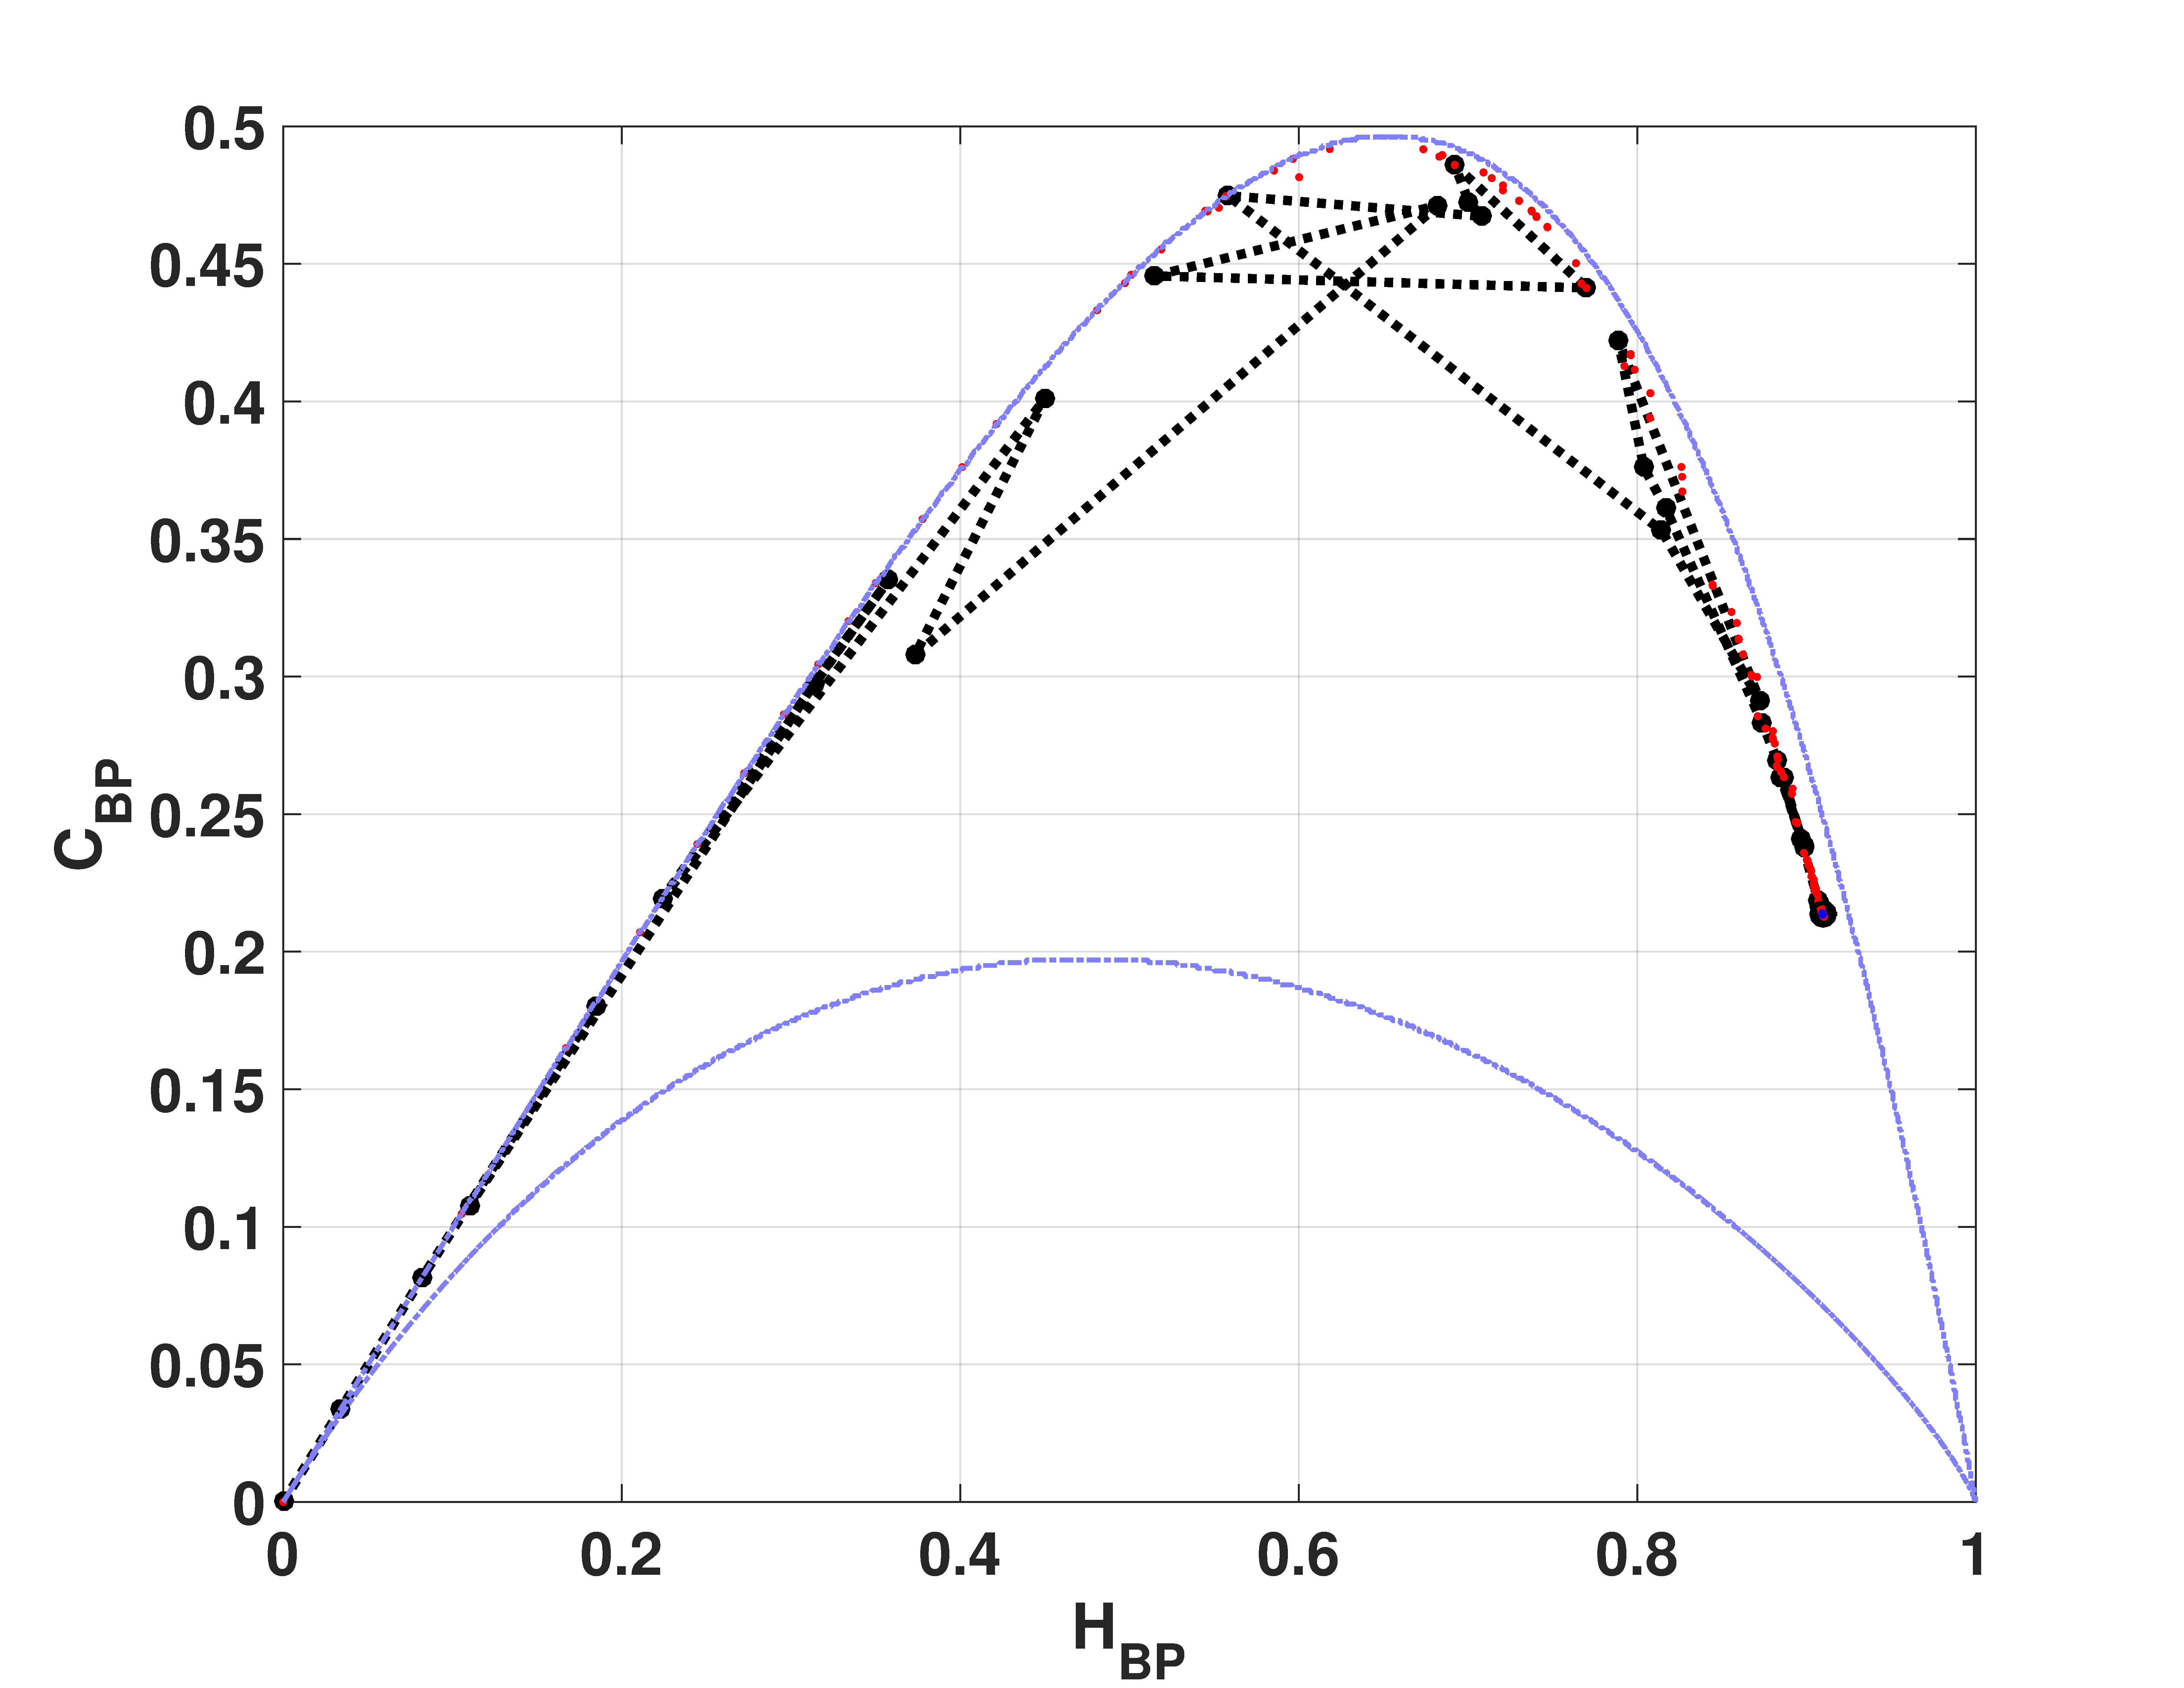
\includegraphics[width=.49\textwidth]{CbpHbp_Odd}
	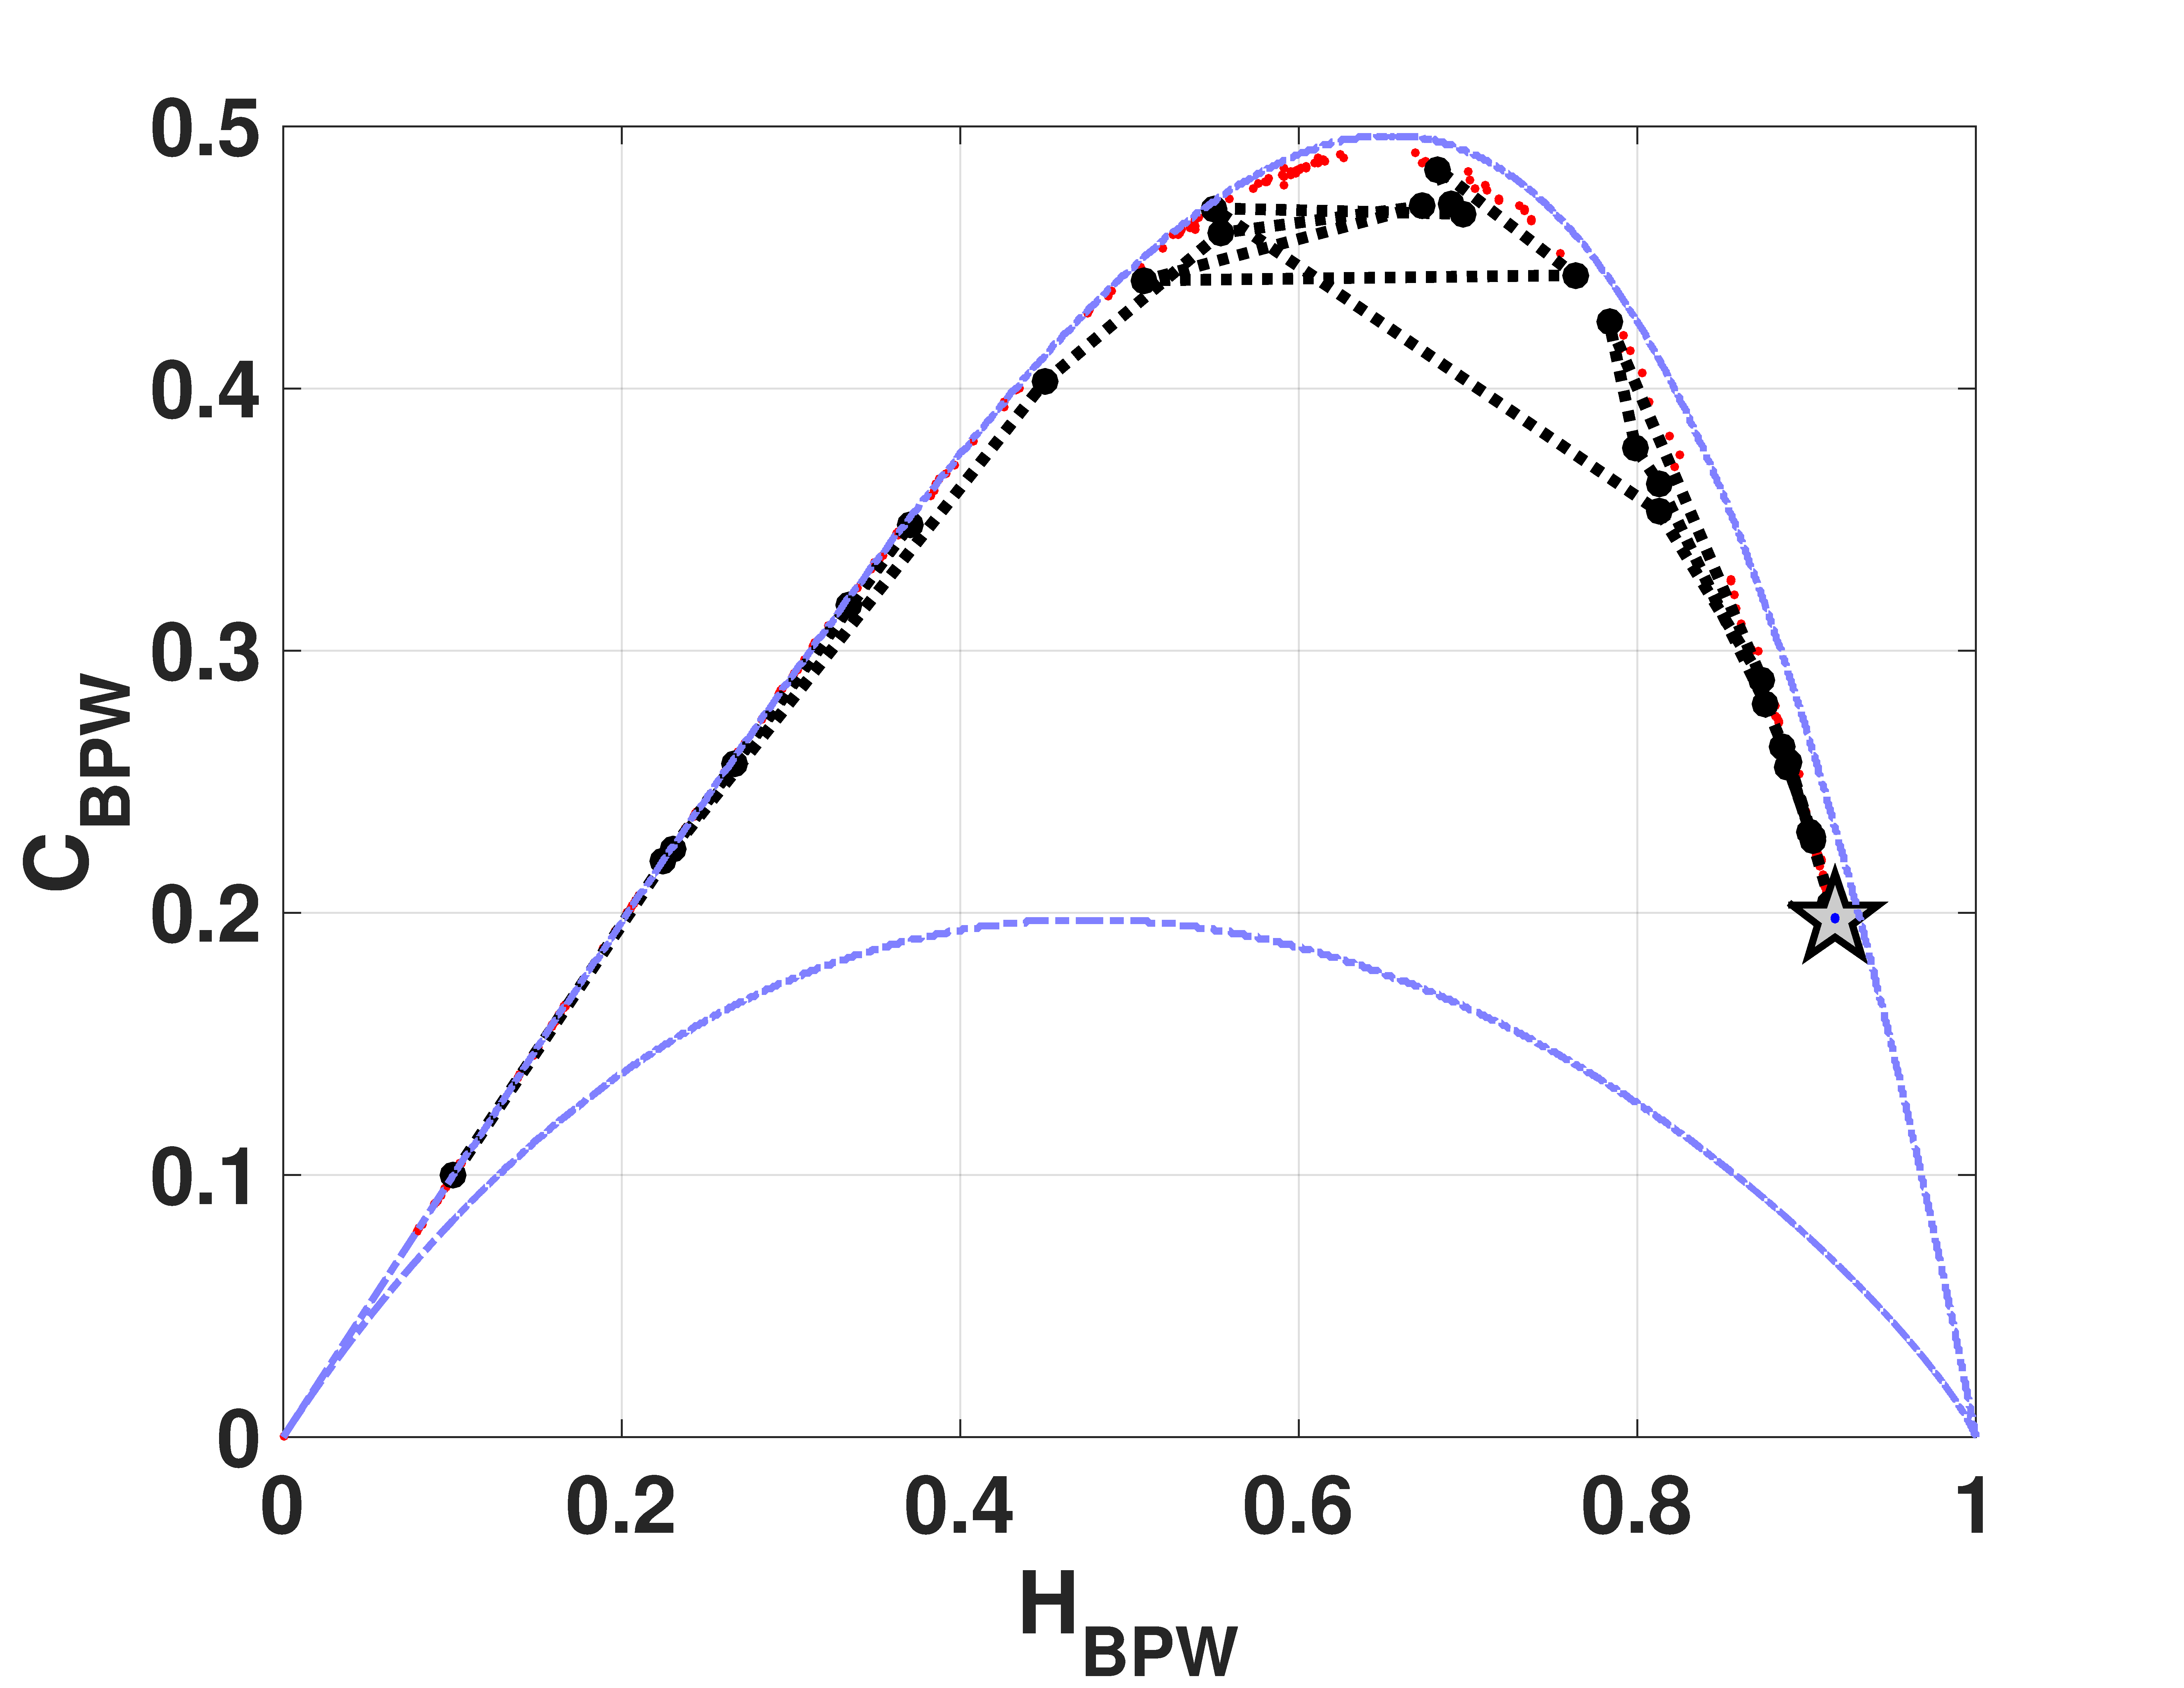
\includegraphics[width=.49\textwidth]{CbpwHbpw_Odd}
	\caption{Evolution of statistical properties in entropy-complexity plane of ODD map: (a) $C_{BP}$ vs $H_{BP}$ (b) $C_{BPW}$ vs $H_{BPW}$.}
	\label{fig:ODD_HC}
\end{figure}